% Generated from main.typ. Typst is authoritative; regeneration overwrites this file.
\documentclass{qlnotes-export}

\title{Math 525: Probability}
\subtitle{Typst-first course notes}
\author{Qiulin Fan}
\date{2026}

\begin{document}
\frontmatter
\maketitle
\tableofcontents

\mainmatter
\chapter{basic combinatorics and probability space}\label{basic-combinatorics-and-probability-space}

\section{permutations and combinations}\label{permutations-and-combinations}

\subsection{permutations}\label{permutations}

% qlnotes: kind=definition; id=def-01-combinatorics-prob-space-permutations; concepts=permutations; aliases=permutations
\begin{definition}{permutations}\label{def-01-combinatorics-prob-space-permutations}

一个 permutation 就是对一组 objects 的一个 \textbf{rearrangement} (这些 objects 中可以有 same 的也可以有 distinct 的).\\
对于 \(n\) 个 \textbf{distinct objects}, 一共存在

\[n! = n(n - 1)(n - 2)\cdots\]

个 permutations.

\end{definition}

% qlnotes: kind=example; id=ex-01-combinatorics-prob-space-example-001; concepts=example-001
\begin{example}\label{ex-01-combinatorics-prob-space-example-001}

求 "STATISTICS" 的 \# distinct permutations.

\end{example}

\begin{qlsolution}{Solution}

这里一共有 10 个 objects. 但问题是: 其中有 3 个 \(S\), 3 个 \(T\), 2 个 \(I\) 是相同的.\\
于是: 我们首先假设它们都是 distinct 的, 则存在 \(10!\) 个 permutations. 而, 每个 permutation 都包含了对 3 个 \(S\) 的一个子 permutation. 而对 3 个 \(S\) 的任意 permutation 都是相同的! 同样的道理 apply to 3 个 \(T\) 和 2 个 \(I\).\\
所以这个结果是真实结果的 \(3!3!2!\) 倍.\\
同样地, 由于 因而, 正确结果是:

\[\frac{10!}{3!3!2!1!1!}\]

\end{qlsolution}

\begin{qlremark}{Remark}

求一组 objects 的 distinct permutations 的数量时, 对于其中相同的 objects, 我们只需要除去它们的重复数量的 factorial (即: 它们自己内部有多少个 permutation 都算作一个 permutation).\\
公式:

\[\frac{n!}{n_{1}!n_{2}!\cdots n_{k}!}\]

其中 \(n_{1},n_{2},\cdots,n_{k}\) 是每个 object 的重复数量.\\
这个式子又叫做 multinomial coefficient.

% qlnotes: kind=definition; id=def-01-combinatorics-prob-space-multinomial-coefficient; concepts=multinomial-coefficient; aliases=multinomial coefficient
\begin{definition}{multinomial coefficient}\label{def-01-combinatorics-prob-space-multinomial-coefficient}

令 \(n \in {\mathbb{N}},n_{1},n_{2},\cdots,n_{k} \in {\mathbb{N}},n_{1} + n_{2} + \cdots + n_{k} = n\), 我们定义 multinomial coefficient:

\[\left( \frac{n}{n_{1},n_{2},\cdots,n_{k}} \right) = \frac{n!}{n_{1}!n_{2}!\cdots n_{k}!}\]

\end{definition}

% qlnotes: kind=proposition; id=prop-01-combinatorics-prob-space-proposition-001; concepts=proposition-001
\begin{proposition}\label{prop-01-combinatorics-prob-space-proposition-001}

如果我们需要 \(n_{1}\) 个 object 1, \(n_{2}\) 个 object 2, \(\cdots\), \(n_{k}\) 个 object \(k\), 那么它们的 distinct permutations 的数量为:

\[\left( \frac{n_{1} + n_{2} + \cdots + n_{k}}{n_{1},n_{2},\cdots,n_{k}} \right)\]

\end{proposition}

\end{qlremark}

\subsection{combinations}\label{combinations}

% qlnotes: kind=definition; id=def-01-combinatorics-prob-space-combinations; concepts=combinations; aliases=combinations
\begin{definition}{combinations}\label{def-01-combinatorics-prob-space-combinations}

一个 combination 就是从一个 set 中选取若干个 elements, 而忽略它们的顺序.

\end{definition}

% qlnotes: kind=proposition; id=prop-01-combinatorics-prob-space-proposition-002; concepts=proposition-002
\begin{proposition}\label{prop-01-combinatorics-prob-space-proposition-002}

从 \(n\) 个 \textbf{distinct objects} 中选取 \(k\) 个的 combinations 的数量为:

\[\left( \frac{n}{k} \right) = \frac{n!}{k!(n - k)!}\]

\end{proposition}

\begin{proof}

我们可以将问题转化为: 从 \(n\) 个 \textbf{distinct objects} 中选取 \(k\) 个的 permutations 的数量, 然后再除去重复的 permutations. 而, 从 \(n\) 个 \textbf{distinct objects} 中选取 \(k\) 个的 permutations 的数量为:

\[n \times (n - 1) \times \cdots \times (n - k + 1) = \frac{n!}{(n - k)!}\]

而其中, 对于每个 valid combination, 都包含了它的所有 ordered permutations, 即重复了 \(k!\) 次. 因此, 最终的结果为:

\[\frac{n!}{k!(n - k)!}\]

\end{proof}

\subsection{binomial theorem}\label{binomial-theorem}

% qlnotes: kind=theorem; id=thm-01-combinatorics-prob-space-binomial-theorem; concepts=binomial-theorem; aliases=Binomial Theorem
\begin{theorem}{Binomial Theorem}\label{thm-01-combinatorics-prob-space-binomial-theorem}

令 \(x,y \in {\mathbb{R}},n \in {\mathbb{N}}\), 则有:

\[(x + y)^{n} = \sum\limits_{k = 0}^{n}\left( \frac{n}{k} \right)x^{n - k}y^{k}\]

\end{theorem}

\begin{proof}

我们可以 prove this by combiinatorial interpretation. 因为把 \(x + y\) 展开即 \(n\) 个 \((x + y)\) 的乘积. 即: 对于每个被乘项, 我们都是在 \(x\) 和 \(y\) 之间选择一个.\\
因而: \(x^{k}y^{n - k}\) 的系数就是从 \(n\) 个 \((x + y)\) 中选取 \(k\) 个 \(x\) 的 combinations 的数量, 即 \(\left( \frac{n}{k} \right)\).\\
考虑所有的 possible \(k\) 值, 我们得到:

\[(x + y)^{n} = \sum\limits_{k = 0}^{n}\left( \frac{n}{k} \right)x^{n - k}y^{k}\]

这是 combinatorial 的 proof.

\end{proof}

另外一种更轮椅的思路是 prove by induction. 这需要一个辅助的 proposition:

% qlnotes: kind=proposition; id=prop-01-combinatorics-prob-space-proposition-003; concepts=proposition-003
\begin{proposition}\label{prop-01-combinatorics-prob-space-proposition-003}

\[\left( \frac{n}{k} \right) = \left( \frac{n - 1}{k - 1} \right) + \left( \frac{n - 1}{k} \right)\]

\end{proposition}

这个等式的 combinatorial interpretation 很 trivial: 对于其中的任意一个 object:

\begin{itemize}
\item
  这个 object 被选中的情况, combinations 的数量: \(\left( \frac{n - 1}{k - 1} \right)\) (从其他里面选 \(k - 1\) 个);
\item
  这个 object 不被选中的情况, combinations 的数量: \(\left( \frac{n - 1}{k} \right)\) (从其他里面选 \(k\) 个).
\end{itemize}

% qlnotes: kind=example; id=ex-01-combinatorics-prob-space-example-002; concepts=example-002
\begin{example}\label{ex-01-combinatorics-prob-space-example-002}

一个 52-card deck, 取 5 张随机牌, 我们获得:

\begin{itemize}
\item
  4 张同 rank 的牌, 最后一张不同 rank 的牌
\item
  a full house (3 张同 rank 的牌, 2 张同 rank 的牌)
\end{itemize}

的概率是多少?

\end{example}

\begin{qlsolution}{Solution}

一共有 \(\left( \frac{52}{5} \right)\) 种取法. 取 4 张同 rank 的牌: 13 种取法. 取最后一张不同 rank 的牌: 52-4 = 48 种取法. 因而, 概率是:

\[\frac{13 \times 48}{\left( \frac{52}{5} \right)}\]

如果是取 3 张同 rank 的牌 + 两张 different 同 rank 的牌: 我们首先在 4 个花色里面选 3 个, 有 \(\left( \frac{4}{3} \right)\) 种取法.\\
因而选取 3 cards of the same rank 的数量为: \(13 \cdot \left( \frac{4}{3} \right)\).\\
然后选取剩余的两张: 然后故技重施, 从剩下的 12 个 rank 里面选 1 个, 而选择它们的花色有 \(\left( \frac{4}{2} \right)\) 种取法. 因而, 概率是:

\[\frac{13 \cdot \left( \frac{4}{3} \right) \cdot 12 \cdot \left( \frac{4}{2} \right)}{\left( \frac{52}{5} \right)}\]

\end{qlsolution}

% qlnotes: kind=example; id=ex-01-combinatorics-prob-space-example-003; concepts=example-003
\begin{example}\label{ex-01-combinatorics-prob-space-example-003}

我们有 \(n\) 把钥匙, 其中有一把是正确的. 尝试 \(k\) 次, 能够成功开门的概率是多少?

\end{example}

\begin{qlsolution}{Solution}

一共有 \(n!\) 种钥匙的 permutations. 我们需要的情况: 正确的钥匙出现在前 \(k\) 个位置:

\begin{itemize}
\item
  正确钥匙出现在第 \(1\) 个位置, 其他 \(n - 1\) 随便排列: \(\cdot (n - 1)!\) 种
\item
  \(\cdots\)
\item
  正确钥匙出现在第 \(k\) 个位置, 其他 \(n - 1\) 随便排列: \(k \cdot (n - 1)!\) 种
\end{itemize}

因而正确的 permutations 的数量为:

\[k \cdot (n - 1)!\]

因而, 概率是:

\[\frac{k \cdot (n - 1)!}{n!} = \frac{k}{n}\]

\end{qlsolution}

\begin{qlremark}{Remark}

正确钥匙出现在每个位置上的概率都是 \(1/n\). 因而它出现在前 \(k\) 个位置的概率就是 \(k/n\).\\
这是一类典型的问题: 不放回的抽取. 在只关心"是否在前 \(k\) 次成功"这一事件时, 这个过程等价于"正确钥匙在一个随机排列中的位置". 这一结果只和比例有关, 与过程细节无关. 只要没有信息bias, 没有偏好, 完全随机, 那么成功概率只取决于:

\begin{itemize}
\item
  你允许的尝试次数 \(k\)
\item
  总可能性数 \(n\)
\end{itemize}

而如果是放回则是不同的情况. 通过补事件容易得:

\[{\mathbb{P}}(A) = 1 - \left( {1 - \frac{1}{n}} \right)^{k}\]

放回和不防回最大的区别是: 放回时, 每次尝试都是独立的, 而不放回时, 每次尝试都不是独立的. 最明显的例子就是, 如果不放回, \(k = n\) 时概率为 1. 而如果放回, 不论 \(k\) 有多大, 概率都小于 1; 当 \(k \ll n\) 的时候, 这两个概率相近 (符合直觉, 因为 \(n\) 很大时放回和不放回几乎没区别.)

\end{qlremark}

% qlnotes: kind=example; id=ex-01-combinatorics-prob-space-example-004; concepts=example-004
\begin{example}\label{ex-01-combinatorics-prob-space-example-004}

一个篮子里有 \(10\) 个 red balls 和 \(5\) 个 blue balls. 我们随机从中取出 \(3\) 个 balls, exactly 其中 \(1\) 个是 blue ball 的概率是多少? 如果每次都放回呢?

\end{example}

\begin{qlsolution}{Solution}

不放回:

\[{\mathbb{P}}(\text{exactly one blue ball}) = \left( \frac{10}{2} \right)\left( \frac{5}{1} \right)\ \ \left( \frac{15}{3} \right) = \frac{45}{91}\]

放回: 5 ways to choose the blue ball, 10 ways to choose the red ball, 以及 3 positions to place the blue ball,

\[{\mathbb{P}}(\text{exactly one blue ball}) = 3 \cdot \frac{3 \cdot 10^{2}}{15^{3}}\]

\end{qlsolution}

\subsection{combinations with repetition}\label{combinations-with-repetition}

% qlnotes: kind=definition; id=def-01-combinatorics-prob-space-combinations-with-repetition; concepts=combinations-with-repetition; aliases=combinations with repetition
\begin{definition}{combinations with repetition}\label{def-01-combinatorics-prob-space-combinations-with-repetition}

一个 combination with repetition 就是从一个 set 中选取若干个 elements, 而忽略它们的顺序, 并且\textbf{允许重复选取}.

\end{definition}

% qlnotes: kind=proposition; id=prop-01-combinatorics-prob-space-proposition-004; concepts=proposition-004
\begin{proposition}\label{prop-01-combinatorics-prob-space-proposition-004}

从 \(n\) 个 \textbf{distinct objects} 中选取 \(k\) 个的 combinations with repetition 的数量为:

\[\left( \frac{n + k - 1}{k} \right)\]

\end{proposition}

\begin{qlremark}{Remark}

关于这个问题我们最开始可能会犯一个错误: 认为 combinations with \(k\) repetitions 的数量为:

\[\left( \frac{kn}{k} \right)\]

但是想一下就知道这是错的. 因为我们相当于给 repeated 的同一个 objects 赋予了顺序, 从而计入了额外的数量.

\end{qlremark}

\begin{proof}

这个问题比较巧妙. 我们上面错误的尝试已经表明: 用 "make copies" 的方法行不通. 我们需要变换一下思路. 原问题是 "要选哪几个元素, 每个元素要选几个". 而我们可以把这个问题理解为: 一共有 \(k\) 个位置, \(n\) 个组, 我们给每个组分配多少个位置?\\
Formalize 这个想法即: 对于第 \(i\) 个 object, 我们给它分配 \(x_{i}\) 个位置. 所有满足条件的 combinations 可以 represent by:

\[\left\{ {y = (x_{1},x_{2},\cdots,x_{n}) \in {\mathbb{Z}}_{\geq 0}^{n}:x_{1} + x_{2} + \cdots + x_{n} = k} \right\}\]

到这里我们想到一个经典的问题: stars and bars. 即: 把 \(k\) 个星星分成 \(n\) 个组, 每个组至少有 1 个星星. 这个问题等价于: 把 \(k\) 个星星和 \(n - 1\) 个隔板排成一排, 然后选择 \(n - 1\) 个隔板的位置.\\
问题是: 我们这里, 一个组可以有 \(0\) 个 stars; 但是这是小问题. 因为我们可以 set \(x_{i}' = x_{i} + 1\), 问题等价转化为:

\[\left\{ {y = (x_{1}',x_{2}',\cdots,x_{n}') \in {\mathbb{Z}}_{\geq 1}^{n}:x_{1}' + x_{2}' + \cdots + x_{n}' = k + n} \right\}\]

这就强制每个组至少有一个 star, 于是可以使用 stars and bars 的方法来解决. 即: 用 \(n - 1\) 个隔板隔开 \(k + n\) 个星星 (有 \(k + n - 1\) 个空档). 因而, 满足条件的 combinations 的数量为:

\[\left( \frac{k + n - 1}{n - 1} \right) = \left( \frac{k + n - 1}{k} \right)\]

\end{proof}

% qlnotes: kind=example; id=ex-01-combinatorics-prob-space-example-005; concepts=example-005
\begin{example}\label{ex-01-combinatorics-prob-space-example-005}

有 5 种口味的 ice creams. 一个人随机选择 20 个 scoops. 求: 每种口味至少被选中一次的 probability.

\end{example}

\begin{qlsolution}{Solution}

即从 \(5\) 种口味中选取 \(20\) 个 combinations with repetition. 于是 sample space 的大小: \(\left( \frac{25 - 1}{20} \right)\).\\
而满足条件的 combinations: 即每种口味我们都预选一个. 然后再从\(5\) 种口味中选取 \(15\) 个 combinations with repetition.

\[{\mathbb{P}}(\text{each flavor is selected at least once}) = \frac{\left( \frac{19}{15} \right)}{\left( \frac{24}{20} \right)} = \frac{\left( \frac{24}{20} \right)}{\left( \frac{24}{20} \right)}\]

\end{qlsolution}

\subsection{inclusion-exclusion principle}\label{inclusion-exclusion-principle}

% qlnotes: kind=proposition; id=prop-01-combinatorics-prob-space-inclusion-exclusion-principle; concepts=inclusion-exclusion-principle; aliases=inclusion-exclusion principle
\begin{proposition}{inclusion-exclusion principle}\label{prop-01-combinatorics-prob-space-inclusion-exclusion-principle}

如果 \(\Omega\) 是一个 finite measure space, 那么对于任意 \(A_{1},\ldots,A_{n} \subseteq \Omega\) 的, 有:

\[\left| {\cup_{i = 1}^{n}A_{i}} \right| = \sum\limits_{i = 1}^{n}\left| A_{i} \right| - \sum\limits_{i < j}\left| {A_{i} \cap A_{j}} \right| + \sum\limits_{i < j < k}\left| {A_{i} \cap A_{j} \cap A_{k}} \right| - \ldots + ( - 1)^{n + 1}\left| {A_{1} \cap \ldots \cap A_{n}} \right|.\]

\end{proposition}

\begin{qlremark}{Remark}

这里的 \(\sum_{i < j}\) 等 index 意思就是\textbf{考虑所有可能的 combinations}, 不考虑顺序, 和下标的顺序没有关系. 比如一共有三个集合 \(A_{1},A_{2},A_{3}\), 那么 \(\left. \sum_{i < j} \middle| A_{i} \cap A_{j}| \right.\) 就是 \(A_{1} \cap A_{2},A_{1} \cap A_{3},A_{2} \cap A_{3}\) 的并集.\\
这个定理是 countable additivity 的直接推广.

\end{qlremark}

% qlnotes: kind=example; id=ex-01-combinatorics-prob-space-example-006; concepts=example-006
\begin{example}\label{ex-01-combinatorics-prob-space-example-006}

(Divisibility) 令 \(n \in {\mathbb{N}}\), 我们随机取一个 \(x \in \left\{ {1,2,\cdots,n} \right\}\), 求 \(x\) is divisible by 2 or 3 or 5 的概率.

\end{example}

\begin{qlsolution}{Solution}

令 \(A_{2},A_{3},A_{5}\) 为 \(x\) 是 2, 3, 5 的倍数的 events. 即:

\[A_{i} = \left\{ {k \in \left\{ {1,2,\cdots,n} \right\} \mid k\ \text{is divisible by}\ i} \right\}\]

于是我们要计算的是:

\[\begin{matrix}
{{\mathbb{P}}(A_{2} \cup A_{3} \cup A_{5})} & {= {\mathbb{P}}(A_{2}) + {\mathbb{P}}(A_{3}) + {\mathbb{P}}(A_{5}) - {\mathbb{P}}(A_{2} \cap A_{3}) - {\mathbb{P}}(A_{2} \cap A_{5}) - {\mathbb{P}}(A_{3} \cap A_{5}) + {\mathbb{P}}(A_{2} \cap A_{3} \cap A_{5})} \\
 & {= \frac{\lfloor\frac{n}{2}\rfloor + \lfloor\frac{n}{3}\rfloor + \lfloor\frac{n}{5}\rfloor - \lfloor\frac{n}{6}\rfloor - \lfloor\frac{n}{10}\rfloor - \lfloor\frac{n}{15}\rfloor + \lfloor\frac{n}{30}\rfloor}{n}}
\end{matrix}\]

\end{qlsolution}

% qlnotes: kind=example; id=ex-01-combinatorics-prob-space-matching-problem; concepts=matching-problem; aliases=(matching problem)
\begin{example}[(matching problem)]\label{ex-01-combinatorics-prob-space-matching-problem}

假设有 \(n\) 个人参加一个 event, 每个人都上交了一顶帽子; 现在再把帽子随机地发给每个人, 求没有人拿回自己的帽子的概率.

\begin{qlsolution}{Solution}

令 \(A_{i}\) 为第 \(i\) 个人拿回自己的帽子的事件. 则我们要求的概率是: \({\mathbb{P}}(\bigcap_{i = 1}^{n}A_{i}^{c})\).

\[\begin{matrix}
{{\mathbb{P}}(\bigcap\limits_{i = 1}^{n}A_{i}^{c})} & {= {\mathbb{P}}((\bigcup\limits_{i = 1}^{n}A_{i})^{c})} \\
 & {= 1 - {\mathbb{P}}(\bigcup\limits_{i = 1}^{n}A_{i})} \\
 & {= 1 - \frac{|\bigcup_{i = 1}^{n}A_{i}|}{n!}}
\end{matrix}\]

由于:

\[\begin{matrix}
{|\bigcup\limits_{i = 1}^{n}A_{i}|} & {= \sum\limits_{i = 1}^{n}\left| A_{i} \right| - \sum\limits_{i < j}\left| {A_{i} \cap A_{j}} \right| + \sum\limits_{i < j < k}\left| {A_{i} \cap A_{j} \cap A_{k}} \right| - \ldots + ( - 1)^{n + 1}\left| {A_{1} \cap \ldots \cap A_{n}} \right|} \\
 & {= \left( \frac{n}{1} \right)(n - 1)! - \left( \frac{n}{2} \right)(n - 2)! + \left( \frac{n}{3} \right)(n - 3)! - \cdots + ( - 1)^{n + 1}} \\
 & {= n!\sum\limits_{k = 1}^{n}( - 1)^{k - 1}\frac{1}{k!}}
\end{matrix}\]

我们可以得到:

\[{\mathbb{P}}(\bigcap\limits_{i = 1}^{n}A_{i}^{c}) = \sum\limits_{k = 2}^{n}\frac{( - 1)^{k}}{k!}\]

\end{qlsolution}

\end{example}

\begin{qlremark}{Remark}

当 \(k\rightarrow\infty\) 的时候, 这个结果趋向于 \(e^{- 1} \approx 0.367879\). (By Taylor's expansion of \(e^{x}\).)

\end{qlremark}

\section{probability space}\label{probability-space}

我们这里跳过所有 measure theory 的内容, 见 notes on measure theory.\\

% qlnotes: kind=definition; id=def-01-combinatorics-prob-space-prob-space-prob-measure-sample-space-event-space; concepts=prob-space-prob-measure-sample-space-event-space; aliases=prob space, prob measure, sample space, event space
\begin{definition}{prob space, prob measure, sample space, event space}\label{def-01-combinatorics-prob-space-prob-space-prob-measure-sample-space-event-space}

一个 probability space 就是一个 measure space \((\Omega,\mathcal{F},{\mathbb{P}})\), 其中 \({\mathbb{P}}(\varnothing) = 0,{\mathbb{P}}(\Omega) = 1\).\\
对于这样的 measure \(\mathbb{P}\), 我们称之为 \textbf{probability measure (概率测度, 即概率)}.\\
而这里的 \(\Omega\) 我们称之为 \textbf{sample space (样本空间)}; 这里的 \(\sigma\)-algebra \(\mathcal{F}\), 我们称之为 \textbf{event space (事件空间)}.\\
任意的 \(A \subset \Omega\) 都是一个 \textbf{event}, 但是概率论中只考虑 \(A \in \mathcal{F}\), 即 measurable event. 为简化, event 这个单词就指 measurable event.

\end{definition}

\begin{qlremark}{Remark}

回顾一下 measure space 的定义:

\begin{itemize}
\item
  一个 set \(\Omega\) 的一个 \(\sigma\)-algebra 就是一个包含空集的子集簇, 其 \textbf{closed under countable unions and complements}. (如果只 closed under finite unions, 则只称为一个 algebra.)
\item
  一个 Borel algebra 是一个定义在 topological space 上的 \(\sigma\)-algebra, 由 all open sets 生成. (因而: closed under countable unions and complements.) \(\mathbb{R}\) 的 Borel algebra 可以由 all open intervals 生成.
\item
  一个 measure on a measurable space \((\Omega,\mathcal{F})\) 就是一个从 \(\mathcal{F}\rightarrow{\mathbb{R}}\) 的函数, 满足 \textbf{countable additivity}.
\item
  measure 的性质: \textbf{(1)non-negativity, (2) monotonicity, (3) countable subadditivity, (4) inclusion-exclusion principle (上节已讲), (5) continuity from below and above.} 第 (5) 条具体即: For measurable sets \(A_{1} \subseteq A_{2} \subseteq \cdots \subseteq A_{n} \subseteq \cdots\), then \(\lim_{n\rightarrow\infty}{\mathbb{P}}(A_{n}) = {\mathbb{P}}(\bigcup_{n = 1}^{\infty}A_{n})\).\\
  For measurable sets \(A_{1} \supseteq A_{2} \supseteq \cdots \supseteq A_{n} \supseteq \cdots\), then \(\lim_{n\rightarrow\infty}{\mathbb{P}}(A_{n}) = {\mathbb{P}}(\bigcap_{n = 1}^{\infty}A_{n})\).
\end{itemize}

\end{qlremark}

\begin{qlremark}{Remark}

对于 discrete 的 prob space 而言, 通常选取 \(\mathcal{F} = 2^{\Omega}\), 即 \(\Omega\) 的任意子集都是一个 event.

\end{qlremark}

\begin{qlremark}{Remark}

概率空间的现实意义是: 一次 experiment 的所有可能的结果的集合, 以及每个结果的概率.

\[\begin{matrix}
\Omega & {= \left\{ {\omega \mid \omega\ \text{是一次 experiment 的可能的结果}} \right\}} \\
{{\mathbb{P}}(\omega)} & {= \text{结果}\ \omega\ \text{的可能性}}
\end{matrix}\]

\end{qlremark}

% qlnotes: kind=example; id=ex-01-combinatorics-prob-space-example-008; concepts=example-008
\begin{example}\label{ex-01-combinatorics-prob-space-example-008}

(dice roll) 如果我们掷一个 6 面的骰子, 那么样本空间 \(\Omega = \left\{ {1,2,3,4,5,6} \right\}\). 一个可能的事件是 \(A = \left\{ {1,2} \right\}\). 如果假设骰子是公平的 (所有结果都是等可能的), 那么事件 \(A\) 的概率是

\[{\mathbb{P}}(A) = \frac{\text{Number of favorable outcomes}}{\text{Total number of outcomes}} = \frac{|A|}{|\Omega|} = \frac{2}{6}\]

根据我们 measure-based 的定义, 这一结果自然 follows from countable additivity of \(\mathbb{P}\).

\end{example}

% qlnotes: kind=example; id=ex-01-combinatorics-prob-space-example-009; concepts=example-009
\begin{example}\label{ex-01-combinatorics-prob-space-example-009}

三个人独立地掷一个 6 面的骰子, 求第三个人掷出的点数等于前两个人的点数之和的概率.

\end{example}

\begin{qlsolution}{Solution}

样本空间 \(\Omega = \left\{ {1,2,3,4,5,6} \right\}^{3}\). event: \(E = \left\{ {\omega \in \Omega \mid \omega_{3} = \omega_{1} + \omega_{2}} \right\}\).\\
这个 event 有 15 个 elements:

\[E = \left\{ {(1,1,2),(1,2,3),(1,3,4),\cdots,(2,1,3),(2,2,4),\cdots,(3,1,4),\cdots,(4,1,5),\cdots,(5,1,6)} \right\}\]

因此, 概率是:

\[{\mathbb{P}}(A) = \frac{|A|}{|\Omega|} = \frac{15}{216} = \frac{5}{72}\]

\end{qlsolution}

% qlnotes: kind=example; id=ex-01-combinatorics-prob-space-example-010; concepts=example-010
\begin{example}\label{ex-01-combinatorics-prob-space-example-010}

两个人计划在 12:00 到 1:00 之间碰面. 他们各自都会在期间的某个时间点到达. 求: 他们彼此不会等待对方超过 10 分钟的概率.\\

\end{example}

\begin{qlsolution}{Solution}

Sample space

\[\Omega = \left\{ {(x,y):0 \leq x \leq 60,0 \leq y \leq 60} \right\} = \lbrack 0,60\rbrack \times \lbrack 0,60\rbrack\]

我们要求概率的事件

\[E = \left\{ (x,y) \in \Omega: \middle| x - y \middle| \leq 10 \right\}\]

容易画出图像:

\begin{figure}
\centering
\pandocbounded{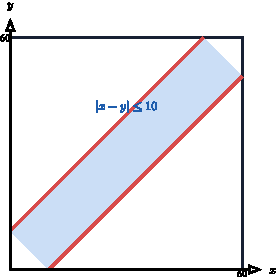
\includegraphics[keepaspectratio,alt={A 60-by-60 arrival-time square with the band abs(x-y) \textless= 10 shaded.}]{assets/fig-prob-01-combinatorics-prob-space-diagram-01.pdf}}
\caption{两人在一小时内到达且等待不超过十分钟的事件区域}\label{fig-prob-01-combinatorics-prob-space-diagram-01}
\end{figure}

因而概率是

\[{\mathbb{P}}(E) = \frac{m(E)}{m(\Omega)} = \frac{3600 - 2500}{3600} = \frac{11}{36}\]

\end{qlsolution}

\subsection{conditional probability and Bayes' theorem}\label{conditional-probability-and-bayes-theorem}

% qlnotes: kind=definition; id=def-01-combinatorics-prob-space-conditional-probability; concepts=conditional-probability; aliases=conditional probability
\begin{definition}{conditional probability}\label{def-01-combinatorics-prob-space-conditional-probability}

对于 probability space \((\Omega,\mathcal{F},{\mathbb{P}})\), 给定一个 event \(B \in \mathcal{F}\), 如果 \({\mathbb{P}}(B) > 0\), 我们定义 conditional probability of an event \(A \in \mathcal{F}\) given \(B\) 为:

\[{\mathbb{P}}(A \mid B) = \frac{{\mathbb{P}}(A \cap B)}{{\mathbb{P}}(B)}\]

\end{definition}

% qlnotes: kind=proposition; id=prop-01-combinatorics-prob-space-decomposing-probability-of-intersection-of-events; concepts=decomposing-probability-of-intersection-of-events; aliases=decomposing probability of intersection of events
\begin{proposition}{decomposing probability of intersection of events}\label{prop-01-combinatorics-prob-space-decomposing-probability-of-intersection-of-events}

令 \(\left( A_{i} \right)_{i \in {\mathbb{N}}}\) 为一个 seq of events, 对于任意 \(n \in {\mathbb{N}}\):

\[{\mathbb{P}}\left( {A_{1} \cap A_{2} \cap \ldots \cap A_{n}} \right) = {\mathbb{P}}\left( A_{1} \right) \cdot {\mathbb{P}}\left( {A_{2} \mid A_{1}} \right) \cdot {\mathbb{P}}\left( {A_{3} \mid A_{1} \cap A_{2}} \right)\ldots \cdot {\mathbb{P}}\left( {A_{n} \mid A_{1} \cap \ldots \cap A_{n - 1}} \right)\]

\end{proposition}

\begin{proof}

Naturally follows from the def.

\end{proof}

% qlnotes: kind=theorem; id=thm-01-combinatorics-prob-space-law-of-total-probability; concepts=law-of-total-probability; aliases=law of total probability
\begin{theorem}{law of total probability}\label{thm-01-combinatorics-prob-space-law-of-total-probability}

令 \(\left( A_{i} \right)_{i \in {\mathbb{N}}}\) 为一个 seq of \textbf{pairwise disjoint} events, 如果 \(\sqcup_{i = 1}^{\infty}A_{i} = \Omega\), 那么对于任意 event \(E \subseteq \Omega\):

\[{\mathbb{P}}(E) = \sum\limits_{i = 1}^{\infty}{\mathbb{P}}\left( A_{i} \right){\mathbb{P}}\left( {E \mid A_{i}} \right)\]

\end{theorem}

\begin{proof}

\[{\mathbb{P}}(E) = {\mathbb{P}}\left( {E \cap \cup_{i = 1}^{\infty}A_{i}} \right) = {\mathbb{P}}\left( {\cup_{i = 1}^{\infty}E \cap A_{i}} \right) = \sum\limits_{i = 1}^{\infty}{\mathbb{P}}\left( {E \cap A_{i}} \right) = \sum\limits_{i = 1}^{\infty}{\mathbb{P}}\left( A_{i} \right){\mathbb{P}}\left( {E \mid A_{i}} \right)\]

\end{proof}

\begin{qlremark}{Remark}

\(P(A_{i})P(E \mid A_{i})\) 就等于 \(P(E \cap A_{i})\), 也就是在 \(A_{i}\) 这个区域上, \(E\) 的 measure. 因而 disjoint union 之下就是 \(E\) 的完整 measure.

\end{qlremark}

% qlnotes: kind=theorem; id=thm-01-combinatorics-prob-space-bayes-theorem; concepts=bayes-theorem; aliases=Bayes theorem
\begin{theorem}{Bayes theorem}\label{thm-01-combinatorics-prob-space-bayes-theorem}

If \(A,B \subseteq \Omega\) such that \({\mathbb{P}}(B) \neq 0\), then

\[{\mathbb{P}}(A \mid B) = \frac{{\mathbb{P}}(A) \cdot {\mathbb{P}}(B \mid A)}{{\mathbb{P}}(B)}\]

\end{theorem}

\begin{qlremark}{Remark}

这其实是一个非常直接的结果, 因为 \(P(A)\dot{P}(B \mid A) = P(A \cap B)\).\\
但是它的意义在于, 如果我们知道两个事件的概率和其中一个对另一个的条件概率, 我们就也得到了反过来的条件概率.

\end{qlremark}

% qlnotes: kind=example; id=ex-01-combinatorics-prob-space-medical-testing; concepts=medical-testing; aliases=(Medical testing)
\begin{example}[(Medical testing)]\label{ex-01-combinatorics-prob-space-medical-testing}

在一个群体中, 随机选取一个人患有某种罕见疾病的概率是 0.001. 该疾病有一个诊断测试, 其性质如下: 给定个体患病, 测试呈阳性的概率 (真正阳性率) 是 0.99. 给定个体健康, 测试呈阳性的概率 (假阳性率) 是 0.02. 从群体中随机选取的一个人测试呈阳性. 该个体实际上患有该疾病的概率是多少? 于是

\begin{qlsolution}{Solution}

由 law of total probability, 我们有

\[{\mathbb{P}}(\text{positive}) = {\mathbb{P}}(\text{positive} \mid \text{sick}){\mathbb{P}}(\text{sick}) + {\mathbb{P}}(\text{positive} \mid \text{healthy}){\mathbb{P}}(\text{healthy}) = 0.99 \cdot 0.001 + 0.02 \cdot 0.999 = 0.02097\]

于是

\[{\mathbb{P}}(\text{sick} \mid \text{positive}) = \frac{0.99 \cdot 0.001}{0.02097} \approx 0.047\]

\end{qlsolution}

\end{example}

% qlnotes: kind=example; id=ex-01-combinatorics-prob-space-monty-hall-problem; concepts=monty-hall-problem; aliases=(Monty Hall problem)
\begin{example}[(Monty Hall problem)]\label{ex-01-combinatorics-prob-space-monty-hall-problem}

假设你参加一个游戏节目, 面前有三扇门: 一扇门后面有一辆车; 其他两扇门后面是山羊. 你选择了一扇门, 比如说是 1 号门, 然后主持人打开了另一扇门, 比如说是 3 号门, 里面有一只山羊. 然后他说 "你想换成 2 号门吗?". 换门对你有利吗?

\begin{qlsolution}{Solution}

令 \(A_{i}\) 表示: car 在 \(i\) 号门后面; \(B\) 事件表示: 主持人打开 3 号门. 我们要求的概率是在事件 \(B\) 发生的情况下, \(A_{2}\) 的个概率, 即 \({\mathbb{P}}(A_{2} \mid B)\). 它的大小是:

\[\begin{matrix}
{{\mathbb{P}}(A_{2} \mid B)} & {= \frac{{\mathbb{P}}(A_{2}) \cdot {\mathbb{P}}(B \mid A_{2})}{{\mathbb{P}}(B)}} \\
 & {= \frac{{\mathbb{P}}(B \mid A_{2}){\mathbb{P}}(A_{2})}{{\mathbb{P}}(B \mid A_{1}){\mathbb{P}}(A_{1}) + {\mathbb{P}}(B \mid A_{2}){\mathbb{P}}(A_{2}) + {\mathbb{P}}(B \mid A_{3}){\mathbb{P}}(A_{3})}} \\
 & {= \frac{1 \cdot \frac{1}{3}}{\frac{1}{2} \cdot \frac{1}{3} + 1 \cdot \frac{1}{3} + 0 \cdot \frac{1}{3}} = \frac{2}{3} > \frac{1}{3}}
\end{matrix}\]

因而, 换门是有利的.

\end{qlsolution}

\begin{qlremark}{Remark}

这是一个非常反直觉的例子. 我们直觉肯定会觉得: 一共 1 辆车和 2 个山羊, 主持人帮忙排除掉了一个山羊, 那么剩下来的两个里面我们二选一, 肯定是 \(1/2\) 概率, 而这个 "更换与否" 就是二选一的抉择. 但其实不是这样的.\\
在第一次选择和第二次选择之间, 主持人带来了额外的信息.

\begin{itemize}
\item
  不换门: win iff 在一开始就选择对了车, 这个概率是 \(1/3\).
\item
  换门: win iff 在一开始选择的是山羊, 这个概率是 \(2/3\).
\end{itemize}

从条件概率的视角来看:

\begin{itemize}
\item
  如果车在 2 号门: 主持人在这个环节里只能选择 3 号门.
\item
  如果车在 1 号门: 主持人在这个环节里可以随机在 2 号和 3 号门里面选择一扇门.
\end{itemize}

也就是说, 主持人打开 3 号门的这个动作, 把 3 号门原本含有的 "中奖潜力" 全部转移给了 2 号门. 这很反直觉. 但是可以用一段 python 程序验证:

\begin{verbatim}
def monty_hall_sim(trials=10000):
    stay_wins = 0
    switch_wins = 0
    for _ in range(trials):
        # 初始化门: 0代表羊, 1代表车 
        doors = [0, 0, 0]
        car_position = random.randint(0, 2)
        doors[car_position] = 1
        
        # 玩家最初的选择
        player_choice = random.randint(0, 2)

        # 主持人打开一扇有山羊的门
        possible_host_doors = [
            i for i in range(3) 
            if i != player_choice and doors[i] == 0
        ]
        host_opens = random.choice(possible_host_doors)

        # 如果"不换"赢了
        if doors[player_choice] == 1:
            stay_wins += 1
        # 如果"换门"赢了
        remaining_door = [
            i for i in range(3) 
            if i != player_choice and i != host_opens
        ][0]
        if doors[remaining_door] == 1:
            switch_wins += 1
    print(f"坚持不换中奖次数: {stay_wins} (概率: {stay_wins/trials:.2%})")
    print(f"换门后中奖次数: {switch_wins} (概率: {switch_wins/trials:.2%})")
\end{verbatim}

运行结果:

\begin{verbatim}
总实验次数: 10000  
坚持不换中奖次数: 3312 (概率: 33.12%)
换门后中奖次数: 6688 (概率: 66.88%)
\end{verbatim}

\end{qlremark}

\end{example}

% qlnotes: kind=example; id=ex-01-combinatorics-prob-space-wizards; concepts=wizards; aliases=(Wizards)
\begin{example}[(Wizards)]\label{ex-01-combinatorics-prob-space-wizards}

两个巫师 \(A\) 和 \(B\) 进行决斗, 他们轮流射击对方. 巫师 \(A\) 每次射击命中 \(B\) 的概率是 \({\mathbb{P}}(A) = \frac{1}{2}\), 而巫师 \(B\) 每次射击命中 \(A\) 的概率是 \({\mathbb{P}}(B) = \frac{2}{3}\). 巫师 \(A\) 先开枪. 求: 巫师 \(A\) 获胜的概率是多少?\\

\begin{qlsolution}{Solution}

任意一轮射击 (假设前一轮没有结束, 于是游戏回到初始状态. 因而任意一轮都是独立的) 中, 令 \(W_{A}\) 为事件: \(A\) 获胜; \(W_{B}\) 为事件: \(B\) 获胜, 假设他们从各自开始射击. 根据全概率公式, 我们有

\[\begin{matrix}
 & {{\mathbb{P}}\left( W_{A} \right) = {\mathbb{P}}(hit){\mathbb{P}}\left( {W_{A} \mid hit} \right) + {\mathbb{P}}(miss){\mathbb{P}}\left( {W_{A} \mid miss} \right) = \frac{1}{2} + \frac{1}{2}{\mathbb{P}}\left( W_{B}^{c} \right)} \\
 & {{\mathbb{P}}\left( W_{B} \right) = {\mathbb{P}}(hit){\mathbb{P}}\left( {W_{B} \mid hit} \right) + {\mathbb{P}}(miss){\mathbb{P}}\left( {W_{B} \mid miss} \right) = \frac{2}{3} + \frac{1}{3}{\mathbb{P}}\left( W_{A}^{c} \right)}
\end{matrix}\]

Solving the system, we find \({\mathbb{P}}\left( W_{A} \right) = 0.6\).

\end{qlsolution}

\begin{qlremark}{Remark}

这个例子表明了先手优势有多大. 相比上一个例子, 这是很直观的.\\
另外, 这个例子有趣的是, 我们把无限的回合转化为了一个循环结构, 利用游戏状态的自相似, 只需要考虑任意一轮即可.

\end{qlremark}

\end{example}

\subsection{Kolmogorov definition of conditional probability}\label{kolmogorov-definition-of-conditional-probability}

我们通过 \({\mathbb{P}}(A \mid B) = \frac{{\mathbb{P}}(A \cap B)}{{\mathbb{P}}(B)}\) 定义出来的 conditional probability 有一个限制, 就是 enforce \({\mathbb{P}}(B) > 0\).\\
但是, 难道 \({\mathbb{P}}(B) = 0\) 就不能定义条件概率了吗? 我们考虑一个连续情况: 在 \({\mathbb{R}}^{3}\) 中任意选择一个点, 求: 该点位于单位球面上的概率. 显然, 这个概率是 0. 但是, 如果我们知道该点位于单位球内, 那么该点距离原点的距离为 \(1\) 的概率应当为 \(1\). 也就是说, 即使在 \({\mathbb{P}}(B) = 0\) 的情况下, 我们也希望定义 \({\mathbb{P}}(A \mid B)\).\\
在考虑这个定义之前, 首先我们发现: 基于我们先前定义的 conditional probability, 我们可以获得一个新的 probability space:

% qlnotes: kind=definition; id=def-01-combinatorics-prob-space-conditional-probability-space-and-trace-sigma-algebra; concepts=conditional-probability-space-and-trace-sigma-algebra; aliases=conditional probability space and trace \sigma-algebra
\begin{definition}{conditional probability space and trace sigma-algebra}\label{def-01-combinatorics-prob-space-conditional-probability-space-and-trace-sigma-algebra}

对于给定的 prob space \((\Omega,\mathcal{F},{\mathbb{P}})\), 给定一个 event \(B \in \mathcal{F}\) 且 \({\mathbb{P}}(B) > 0\), 我们定义 conditional probability space as the triplet \((B,\mathcal{F}_{B},{\mathbb{P}}( \cdot \mid B))\), 其中:

\[F_{B} := \left\{ {A \cap B \mid A \in \mathcal{F}} \right\}\]

被称为 \textbf{trace \(\sigma\)-algebra on \(B\)}.\\
容易验证, 这个 triplet 是一个 prob space.

\end{definition}

\begin{qlremark}{Remark}

当我们把整个 prob space 限制在 event \(B\) 上时, 本质上是在做一个 Radon-Nikodym derivative 的操作.\\
定义 \(f := \frac{{\mathbb{I}}_{B}}{{\mathbb{P}}(B)}\), 那么对于任意 event \(A \in \mathcal{F}_{\mathcal{B}}\), 有:

\[{\mathbb{P}}(A \mid B) = \int_{A}f\, d{\mathbb{P}}\]

因而和我们的直觉一样, 条件概率是通过一个 density function 来重新加权原本的概率测度.

\end{qlremark}

既然这样, 我们能否直接从一个新的 prob space \((B,\mathcal{F}_{B},{\mathbb{P}}( \cdot \mid B))\) 出发, 来定义条件概率呢? 这就是 Kolmogorov 的定义:

% qlnotes: kind=definition; id=def-01-combinatorics-prob-space-kolmogorov-definition-of-conditional-probability; concepts=kolmogorov-definition-of-conditional-probability; aliases=Kolmogorov definition of conditional probability
\begin{definition}{Kolmogorov definition of conditional probability}\label{def-01-combinatorics-prob-space-kolmogorov-definition-of-conditional-probability}

对于给定的 prob space \((\Omega,\mathcal{F},{\mathbb{P}})\), 设 \(\mathcal{G} \subseteq \mathcal{F}\) 是一个 sub-\(\sigma\)-algebra. 对于 event \(A \in \mathcal{F}\), 条件概率 \({\mathbb{P}}(A \mid \mathcal{G})\) 是一个 \(\mathcal{G}\)-measurable 的随机变量, 其满足对于任意 \(G \in \mathcal{G}\), 有:

\[\int_{G}{\mathbb{P}}(A \mid \mathcal{G})\, d{\mathbb{P}} = {\mathbb{P}}(A \cap G)\]

显然, 当 \({\mathbb{P}}(B) > 0\) 时, 这个定义和我们之前的定义是等价的.\\
这个 random variable \({\mathbb{P}}(A \mid \mathcal{G})\) 在 \(\mathbb{P}\)-a.s. 意义下是唯一的.

\end{definition}

\begin{qlremark}{Remark}

条件概率 \({\mathbb{P}}(A \mid \mathcal{G})\) 这个测度是 \({\mathbb{P}}(A \cap \cdot )\) 这个测度相对于背景测度 \(\mathbb{P}\) 在子信息流 \(\mathcal{G}\) 下的 Radon-Nikodym derivative, 也就是一个密度函数.\\
这个定义里没有指明, 给定一个 event \(B \in \mathcal{F}\), 如何去确定 \(\mathcal{G}\) 以及 \({\mathbb{P}}(A \mid \mathcal{G})\). 虽然这是一个抽象的存在性{ } 唯一性定义, 但是标准的做法是:

\begin{itemize}
\item
  看向产生 \(B\) 的 random variable \(X\), 即 \(B = \left\{ {X = x} \right\}\), 令 \(\mathcal{G} = \sigma(X)\), 即由 random variable \(X\) 生成的 \(\sigma\)-algebra. 这个 \(\sigma\)-algebra 包含了所有关于 \(X\) 可能取值的信息.
\item
  既然 \({\mathbb{P}}(A \mid \sigma(X))\) 是关于 \(\sigma(X)\) 可测的, 那么它一定可以写成 \(h(X)\) 的形式. 通过对 \(X\) 的所有可能取值进行积分, 我们确定了函数 \(h( \cdot )\) 的整体形态, 这时我们定义 \(P(A \mid X = x)\) 为函数 \(h\) 在点 \(x\) 处的值.
\item
  \({\mathbb{P}}(A \mid \mathcal{G})\) 实际就是条件期望 \({\mathbb{E}}\lbrack{\mathbb{I}}_{A} \mid \mathcal{G}\rbrack\). 当 \({\mathbb{P}}(B) > 0\) 时, 它就退化回经典定义 \(\frac{{\mathbb{P}}(A \cap B)}{{\mathbb{P}}(B)}\).
\end{itemize}

\end{qlremark}

\begin{qlremark}{Remark}

Further issue: \textbf{Borel-Kolmogorov paradox}.\\
即便是这个定义, 也会出现问题.\\
给定一个事件 \(B\), 如果 \({\mathbb{P}}(B) = 0\), 则 \({\mathbb{P}}(A \mid B)\) 的取值取决于我们将 \(B\) 嵌入到哪一个随机变量 \(X\) 中. 不同的随机变量 \(X,Y\) 即使都能产生相同的事件 \(\left\{ {X = x} \right\} = \left\{ {Y = y} \right\} = B\), 它们生成的子 \(\sigma\)-代数 \(\sigma(X)\) 和 \(\sigma(Y)\) 却不同, 导致最终确定的条件概率 \(h_{X}(x) \neq h_{Y}(y)\).\\
为了解决这个问题, 可以引入更精细的结构, 比如说 regular conditional probability, 以及 disintegration theorem. 不过此处不展开了.

\end{qlremark}

\subsection{independence of events}\label{independence-of-events}

% qlnotes: kind=definition; id=def-01-combinatorics-prob-space-independence-of-events; concepts=independence-of-events; aliases=independence of events
\begin{definition}{independence of events}\label{def-01-combinatorics-prob-space-independence-of-events}

对于 prob space \((\Omega,\mathcal{F},{\mathbb{P}})\), 两个 events \(A,B \in \mathcal{F}\) 如果有

\[{\mathbb{P}}(A \cap B) = {\mathbb{P}}(A) \cdot {\mathbb{P}}(B)\]

则称 \(A\) 和 \(B\) 是 independent 的.\\
更加 generally, 对于任意 collection of events \(\left\{ A_{i} \right\}_{i \in I}\), 如果对于任意有限子集 \(J \subseteq I\), 有

\[{\mathbb{P}}\left( {\bigcap\limits_{j \in J}A_{j}} \right) = \prod\limits_{j \in J}{\mathbb{P}}(A_{j})\]

则称 \(\left\{ A_{i} \right\}_{i \in I}\) 是 mutually independent 的.

\end{definition}

\begin{qlremark}{Remark}

根据条件概率的定义, 容易得出: 两个 events \(A,B\) independent 的定义\textbf{等价于 \({\mathbb{P}}(A \mid B) = {\mathbb{P}}(A)\)}, 即事件 \(B\) 的发生与否不影响事件 \(A\) 发生的概率.\\

% qlnotes: kind=proposition; id=prop-01-combinatorics-prob-space-independence-of-two-events; concepts=independence-of-two-events; aliases=independence of two events 的等价定义
\begin{proposition}{independence of two events 的等价定义}\label{prop-01-combinatorics-prob-space-independence-of-two-events}

对于 prob space \((\Omega,\mathcal{F},{\mathbb{P}})\), 两个 events \(A,B \in \mathcal{F}\) independent iff:

\[{\mathbb{P}}(B \mid A) = {\mathbb{P}}(B)\]

\end{proposition}

\begin{proof}

Directly follows from the definition of conditional probability.

\end{proof}

因而 independence of two events 的定义等价于: 事件 \(A\) 的发生与否不影响事件 \(B\) 发生的概率 (反之亦然).

将它推广到多个事件: 即\textbf{任意一个事件的发生与否都不影响其他事件发生的概率}.

\end{qlremark}

\begin{qlremark}{Remark}

我们从 measure 的角度看待两个事件的 independence: 首先 \({\mathbb{P}}(B) = 0\) 是 trivial case, 而 如果 \({\mathbb{P}}(B) > 0\), 那么 independence 其实可以化为一个等式:

\[\frac{{\mathbb{P}}(A \cap B)}{{\mathbb{P}}(B)} = \frac{{\mathbb{P}}(A)}{{\mathbb{P}}(\Omega)}\]

意思是: 事件 \(A\) 在 \(B\) 这个 set 中占据的 measure 比例, 完全等于事件 \(A\) 在整个空间 \(\Omega\) 中占据的 measure 比例; 也就是说, \textbf{事件 \(B\) 的发生并没有改变事件 \(A\) 在空间中的 measure 分布.}

因而, 这两个集合在 measure (probability) 的意义下是完全解耦的, 这就是 independence 的 information geometric 意义.

\end{qlremark}

% qlnotes: kind=proposition; id=prop-01-combinatorics-prob-space-proposition-008; concepts=proposition-008
\begin{proposition}\label{prop-01-combinatorics-prob-space-proposition-008}

如果 events \(A\) 和 \(B\) independent, 则 \(A\) 和 \(B^{c}\) 也是 independent 的.

\end{proposition}

\begin{proof}

\[\begin{matrix}
{{\mathbb{P}}\left( {A^{c} \cap B^{c}} \right)} & {= {\mathbb{P}}\left( {(A \cup B)^{c}} \right) = 1 - {\mathbb{P}}(A \cup B) = 1 - {\mathbb{P}}(A) - {\mathbb{P}}(B) + {\mathbb{P}}(A \cap B)} \\
 & {= 1 - {\mathbb{P}}(A) - {\mathbb{P}}(B) + {\mathbb{P}}(A) \cdot {\mathbb{P}}(B) = (1 - {\mathbb{P}}(A))(1 - {\mathbb{P}}(B))} \\
 & {= {\mathbb{P}}\left( A^{c} \right) \cdot {\mathbb{P}}\left( B^{c} \right)}
\end{matrix}\]

\end{proof}

% qlnotes: kind=example; id=ex-01-combinatorics-prob-space-pairwise-independence-vs-mutual-independence; concepts=pairwise-independence-vs-mutual-independence; aliases=(Pairwise Independence vs. Mutual Independence)
\begin{example}[(Pairwise Independence vs.~Mutual Independence)]\label{ex-01-combinatorics-prob-space-pairwise-independence-vs-mutual-independence}

一组事件 \(A_{1},A_{2},\ldots \in \mathcal{F}\) 如果是 mutually independent 的, 则它们两两 independent. \textbf{但是反过来不成立}.\\
即: \textbf{即便对于任意 \(i \neq j\), 有 \({\mathbb{P}}(A_{i} \cap A_{j}) = {\mathbb{P}}(A_{i}){\mathbb{P}}(A_{j})\), 也并不意味着这些事件是 mutually independent 的}.\\
下面为一个 counterexample: 考虑掷两个骰子. 令事件

\[A := \left\{ {\text{first roll is}\ 4} \right\},\quad B := \left\{ {\text{second roll is}\ 3} \right\},\quad C := \left\{ {\text{the sum of the two outcomes is}\ 7} \right\}\]

我们发现: \({\mathbb{P}}(A \cap B \cap C) = \frac{1}{36} \neq {\mathbb{P}}(A){\mathbb{P}}(B){\mathbb{P}}(C) = \frac{1}{6^{3}}\), 因而 \(A,B,C\) 并不 mutually independent. 然而, However, \({\mathbb{P}}(A \cap B) = \frac{1}{36} = {\mathbb{P}}(A){\mathbb{P}}(B),{\mathbb{P}}(A \cap C) = \frac{1}{36} = {\mathbb{P}}(A){\mathbb{P}}(C)\) and \({\mathbb{P}}(B \cap C) = \frac{1}{36} = {\mathbb{P}}(B){\mathbb{P}}(C)\), 因而它们两两 pairwise independent.

\end{example}

\begin{qlremark}{Remark}

这个反例能够成功的理由是: 事件 \(C\) (总和) 和 事件 \(A\) (第一个骰子) 以及事件 \(B\) (第二个骰子) 分别都是独立的, 因为知道了其中一个并不会影响另一个的概率. 但是, 一旦我们知道了 \(A\) 和 \(B\) 的值, 那么 \(C\) 的值就被完全确定了 (因为总和就是两个骰子的和). 因而, 三个事件并不 mutually independent.\\
(注意: 如果 \(C\) 事件不是和为 7 而是一个小于 7 的数, 那就不是了, 因为如果我们知道第一次是 6, 那么和就不可能是 6, 那么就也失去了 pairwise independence).\\
这个例子说明了, mutual independence 是一个比较强的条件. 我们可以把这三个事件看作是对结果空间的约束:

\begin{itemize}
\item
  两个骰子的结果空间有 36 个点.
\item
  \(A\) 是一条线 (6个点), \(B\) 是另一条线 (6个点), \(C\) 是一条对角线 (6个点)。
\item
  两两独立: 意味着任意两条线相交的点数, 恰好符合概率乘积.
\item
  相互独立: 要求这三条线交于一点的概率也符合乘积.
\end{itemize}

这个例子提醒我们: 独立性不是一种可以由低维向高维简单``归纳''的性质. 一个系统可以局部解耦（两两独立, 但在全局尺度上却存在强耦合. 总之 mutual independence 是一个很强的条件.

\end{qlremark}

% qlnotes: kind=example; id=ex-01-combinatorics-prob-space-coin-tossing; concepts=coin-tossing; aliases=(coin tossing)
\begin{example}[(coin tossing)]\label{ex-01-combinatorics-prob-space-coin-tossing}

假设我们有一枚不均匀的硬币, 掷出正面的概率是 \(p \in \lbrack 0,1\rbrack\), 反面的概率是 \(1 - p\). 我们不断地掷这枚硬币, 直到第一次掷出正面为止, 并记录所需的掷币次数. 求: 掷币次数为奇数的概率是多少?

\begin{qlsolution}{Solution}

对于任意 \(i \in {\mathbb{N}}\), 考虑事件 \(A_{i} = \{\) 掷币次数为 \(i\}\).

\[{\mathbb{P}}\left( {\cup_{n = 1}^{\infty}A_{2n - 1}} \right) = \sum\limits_{n = 1}^{\infty}{\mathbb{P}}\left( A_{2n - 1} \right) = \sum\limits_{n = 1}^{\infty}(1 - p)^{2n - 2}p = p\sum\limits_{n = 1}^{\infty}\left( {(1 - p)^{2}} \right)^{n - 1} = p \cdot \frac{1}{1 - (1 - p)^{2}} = \frac{1}{2 - p}\]

\end{qlsolution}

\begin{qlremark}{Remark}

这个问题还可以通过 law of total probability 来解决.\\
令 \(E =\) 掷币次数为奇数. 那么

\[\begin{matrix}
{{\mathbb{P}}(E)} & {= {\mathbb{P}}(\text{head}) \cdot {\mathbb{P}}(E \mid \text{head}) + {\mathbb{P}}(\text{tail}) \cdot {\mathbb{P}}(E \mid \text{tail})} \\
 & {= p \cdot 1 + (1 - p) \cdot (1 - {\mathbb{P}}(E))}
\end{matrix}\]

Solve 这个 equation 得到同样结果.

\end{qlremark}

\end{example}

\chapter{random variable}\label{random-variable}

\section{\texorpdfstring{random variable and generated \(\sigma\)-algebra}{random variable and generated \textbackslash sigma-algebra}}\label{random-variable-and-generated-sigma-algebra}

\subsection{random variable: 即 prob space 上的一个 Borel measurable function}\label{random-variable-ux5373-prob-space-ux4e0aux7684ux4e00ux4e2a-borel-measurable-function}

% qlnotes: kind=definition; id=def-02-random-variables-random-variable; concepts=random-variable; aliases=random variable
\begin{definition}{random variable}\label{def-02-random-variables-random-variable}

对于 probability space \((\Omega,\mathcal{F},{\mathbb{P}})\), 一个 random variable 是一个 \textbf{Borel measurable function} \(X:\Omega\rightarrow{\mathbb{R}}\).

\end{definition}

\begin{qlremark}{Remark}

回顾 (Borel) measurable function 的定义: 即对于任意 \(B \in \mathcal{B}({\mathbb{R}})\), 有 \(X^{- 1}(B) \in \mathcal{F}\); 由于是在 real space 上, Borel measurable 也可以简化为: 对于任意的 open ray \(( - \infty,a)\), 有 \(X^{- 1}(( - \infty,a)) \in \mathcal{F}\).

例如: \(X(\omega) = \omega^{2}\) 是一个 (Borel) measurable function, 因为对于任意 open ray \(( - \infty,a)\), \(X^{- 1}(( - \infty,a))\) 是一个 interval (either \(( - \sqrt{a},\sqrt{a})\) or \(\varnothing\)).

并且 recall: 任意的 continuous function 都是 (Borel) measurable function. (所以之后我们看到 continuous function 就知道它一定是一个 random variable).

\end{qlremark}

\begin{qlremark}{Remark}

Random variable (Borel measurable function) 本质上是对 样本空间中的事件进行 weights assignment.

原本, 一个 prob space 只能表示: \textbf{有多少个 outcomes, 每个 outcome 的概率是多少} (对于无限的 sample space, 一些 outcomes 组合, 即事件, 的概率是多少).

而 random variable 就是\textbf{给这些 outcomes 以 weights}: 比如

% qlnotes: kind=example; id=ex-02-random-variables-example-001; concepts=example-001
\begin{example}\label{ex-02-random-variables-example-001}

在一副扑克牌中抽一张, 那么每一张的概率都是 \(1/52\). 但是如果我想知道抽到的牌的价值, 那么我就需要一个 random variable \(X\) 来给每一张牌赋予一个 weight; 比如说, \(X(\text{A}) = 1\), \(X(2) = 2\), \(\cdots\), \(X(\text{K}) = 13\).\\

\end{example}

\textbf{Question}: 为什么对于 assigning weights 的行为, 我们一定要求它是一个 (Borel) measurable function 呢? 普通的给 outcomes 以 weights 的行为 (任意一个 function \(f:\Omega\rightarrow{\mathbb{R}}\)) 不行吗?

\textbf{Answer}: 因为我们想要知道 \(X\) 的值在一个范围 \(B\), 比如 \(\lbrack 1,6\rbrack\) 之内的 probability (which is defined on 原本的 prob measure \(\mathbb{P}\) 上的) 是多少. 而只有每一个这样的范围集合的 preimage \(X^{- 1}(B)\) 都是 \(\mathcal{F}\) 中的事件, 我们才能够通过 \(\mathbb{P}\) 来计算这个 probability; that is, 我们需要这个 \(X\) 是一个 measurable function.

因为这一切都是建立在我们以 measure theory 的 framework 来定义 probability 的基础上的.\\

\end{qlremark}

下面是一个简单的 proposition: 我们可以把多个 random variables 以一种 Borel measurable 的方式组合起来, 那么就成为一个新的 random variable.

% qlnotes: kind=proposition; id=prop-02-random-variables-borel-measurable-random-variables; concepts=-borel-measurable-random-variables; aliases=以 Borel measurable 的方式组合起多个 random variables
\begin{proposition}{以 Borel measurable 的方式组合起多个 random variables}\label{prop-02-random-variables-borel-measurable-random-variables}

Prob space \((\Omega,\mathcal{F},{\mathbb{P}})\) 上的 random variables \(X_{1},X_{2},\ldots,X_{k}:\Omega\rightarrow{\mathbb{R}}\), 任取 Borel measurable function \(g:{\mathbb{R}}^{k}\rightarrow{\mathbb{R}}\),

\[\begin{matrix}
{X:\Omega} & {\rightarrow{\mathbb{R}}} \\
\omega & {\mapsto g(X_{1}(\omega),X_{2}(\omega),\ldots,X_{k}(\omega))}
\end{matrix}\]

也是一个 random variable.

\end{proposition}

\begin{proof}

我们在 measure theory 中证明过: 对于任意的 finite seq of Borel measureable functions \((f_{i}:\Omega\rightarrow{\mathbb{R}})_{i = 1}^{k}\), 其各作为一个维度组成的函数 \(f = (f_{1},\cdots,f_{k})\) 也是一个 Borel measurable function (from \(\Omega\) 到 \({\mathbb{R}}^{k}\)).\\
而这里的 \(X\) 就是 \(g \circ f\), 是两个 Borel measurable function 的 composition, 因而也是一个 Borel measurable function (即 random variable).

\end{proof}

\begin{qlremark}{Remark}

以一种 Borel measurable 的方式组合多个 random variables, 这个函数也仍然是一个 random variable.

这个 proposition 看似没有什么卵用, 但是它其实是我们之后构造 random variable 的一个重要工具. 很多我们默认合法的行为, 它都作为基础.

比如我们:

\begin{itemize}
\item
  定义了两个 random variable \(X\) 和 \(Y\), 那么它们的和 \(X + Y\) 以及积 \(X \cdot Y\) 也是 random variables.
\item
  更加复杂的: 标量变换 \(g(X) = \sin(X),h(X) = e^{X}\), 向量变换 \(g(X_{1},X_{2}) = X_{1}^{2} + X_{2}^{2}\), 等等, 都是 random variables.
\item
  统计学中, 我们有一堆样本, \textbf{每一个都是随机采样得到的 (即一个 random variable \(X_{i}\))}. 因而在观测之前, 我们 把它看作一个 random variable \(X_{i}\), 然后在观测之后取到它的一个实际值 \(x_{i}\).

  通常我们假设所有样本都是 \textbf{independent and identically distributed (i.i.d., 独立同分布)} 的, 即所有的 \(X_{1},X_{2},\ldots,X_{n}\) 都是 independent 的, 并且服从同一个 distribution (discuss later\ldots).

  然后, 我们就可以从这些样本中计算各种统计量, 比如平均值 \(\bar{X} := \frac{1}{n}\sum_{i = 1}^{n}X_{i}\), 再比如 order statistic, sample variance 等等, 从而通过大数定律等工具的辅佐, 来估计这个 distribution 到底是什么样的一个 distribution.

  这里这些统计量, 由于是以 Borel measurable 的方式组合起多个 random variables, 也是 random variables. 所以这个 proposition 其实也奠定了统计学中各种统计量的合法性.
\end{itemize}

\end{qlremark}

\subsection{\texorpdfstring{由一个 random variable generate 的 \(\sigma\)-algebra}{由一个 random variable generate 的 \textbackslash sigma-algebra}}\label{ux7531ux4e00ux4e2a-random-variable-generate-ux7684-sigma-algebra}

% qlnotes: kind=definition; id=def-02-random-variables-sigma-algebra-generated-by-a-random-variable-measurable-function; concepts=sigma-algebra-generated-by-a-random-variable-measurable-function; aliases=\sigma-algebra generated by a random variable (measurable function)
\begin{definition}{sigma-algebra generated by a random variable (measurable function)}\label{def-02-random-variables-sigma-algebra-generated-by-a-random-variable-measurable-function}

对于 random variable \(X:\Omega\rightarrow{\mathbb{R}}\), 其 generate 的 \(\sigma\)-algebra 定义为

\[\sigma(X) := \left\{ {X^{- 1}(B):B \in \mathcal{B}({\mathbb{R}})} \right\} \subseteq \mathcal{F}\]

\end{definition}

这个集合 \(\sigma(X)\) 是一个 \(\sigma\)-algebra, 是一个 trivial truth. 因为 里面所有的 set 都是 \(X\) 的 preimage, 而 \(X\) 是一个 measurable function, 因而任意的 \(X^{- 1}(B) \in \mathcal{F}\).

这个 \(\sigma(X)\) 也是让 \(X\) 成为一个 measurable function (即 random variable) 的最小的 \(\sigma\)-algebra. 它的意义是: \textbf{当我们仅仅观察到 \(X\) 的取值时, 我们所掌握的关于 underlying sample space \(\Omega\) 的全部 "information".}

\begin{qlremark}{Remark}

我们知道, \textbf{一个 \(\sigma\)-algebra \(\mathcal{F}\) 可以看作是一个 information structure}: 它是对 underlying sample space \(\Omega\) 进行划分的一个工具.\\
最大的 \(\sigma\)-algebra \(\mathcal{P}(\Omega)\), 即 power set, 是 最细的划分, 也是信息量最大的 \(\sigma\)-algebra. 它把每一个元素都区分开来. 对于 discrete 的 sample space, 通常我们的 probability measure 就是定义在 power set 上的, 正是因为我们 希望区分每一个 outcome.\\
而给定一个 prob space \((\Omega,\mathcal{F},{\mathbb{P}})\), 原本的 prob measure 所 base on 的 \(\sigma\)-algebra \(\mathcal{F}\) 就成为了一个基准的 information 的颗粒度: 哪些事件是我们可以区分, 即可以在上面定义 probability 的.

而一个 random variable \(X\) 可能会把多个 outcomes 映射到同一个值上, 也即 把多个 events 映射到同一个值上, 从而把这些 events 区分不开来. 因而, \textbf{random variable \(X\) generate 的 \(\sigma\)-algebra \(\sigma(X)\) 就可能是一个更粗的划分}. 当我们取这些 events 所映射到的同一个值的 preimage 的时候, 取到的是 它们的 union, 也就是它们中最大的一个.

比如

% qlnotes: kind=example; id=ex-02-random-variables-example-002; concepts=example-002
\begin{example}\label{ex-02-random-variables-example-002}

掷一次骰子, 所有可能结果为 sample space:

\[\Omega = \left\{ {1,2,3,4,5,6} \right\}\]

而我们定义一个 random variable \(X\) 来表示掷出的点数的奇偶性, 即:

\[X(\omega) = \left\{ \begin{matrix}
{1,} & {\omega \in \left\{ {2,4,6} \right\}} \\
{0,} & {\omega \in \left\{ {1,3,5} \right\}}
\end{matrix} \right.\]

那么它 generate 的 \(\sigma\)-algebra:

\[\sigma(X) = \ \varnothing,\left\{ {1,3,5} \right\},\left\{ {2,4,6} \right\},\Omega\ \]

因为 \(1,3,5\) 这些事件都被映射到了同一个值 \(0\) 上, 即 \(\left\{ 1 \right\},\left\{ 3 \right\},\left\{ 5 \right\},\left\{ {1,3} \right\}\) 这些事件都被 \(\left\{ {1,3,5} \right\}\) 这个 事件吸收了, 它们在这个 random variable \(X\) 的映射下是区分不开的. 这就代表了 这个 random variable 所蕴含的信息颗粒度: \textbf{我们只能区分掷出的点数是奇数还是偶数, 但是无法区分具体的点数是多少.}\\
至此我们知道: \textbf{一个 random variable \(X\) 的 generate 的 \(\sigma\)-algebra \(\sigma(X)\) 表示了这个 random variable 对 underlying sample space \(\Omega\) 所能区分的 information granularity (信息颗粒度)}.\\

\end{example}

\end{qlremark}

除了能表示 information granularity 以外, \(\sigma(X)\) 还有什么实际用处呢:

\begin{itemize}
\item
  之后讨论关于 independence of two random variables \(X\) 和 \(Y\) 时, 可以用它来作严格定义, 并且展现 independence 的本质: 两个 RV 的 independence 实际表示它们蕴含的信息颗粒度之间没有任何 overlap
\item
  用以定义 conditional expectation: \(\left. {\mathbb{E}}\lbrack Y \middle| \sigma(X)\rbrack \right.\), 通常 简写为 \(\left. {\mathbb{E}}\lbrack Y \middle| X\rbrack \right.\), 但是其实 \(\left. {\mathbb{E}}\lbrack Y \middle| \sigma(X)\rbrack \right.\) 是一个更加直观的事情, 表述了一种 Partial Averaging 的概念.
\item
  Stochastic Process 中有众多应用. 比如 stopping time 的定义.
\end{itemize}

至此关于 random variable, 我们已经讨论了很多 general 的 刻画. 现在我们来讲一点实用的:

\section{distributions}\label{distributions}

\subsection{distribution and cumulative distribution function}\label{distribution-and-cumulative-distribution-function}

% qlnotes: kind=definition; id=def-02-random-variables-probability-distribution; concepts=probability-distribution; aliases=probability distribution
\begin{definition}{probability distribution}\label{def-02-random-variables-probability-distribution}

对于 random variable \(X:\Omega\rightarrow{\mathbb{R}}\) on \(\Omega,\mathcal{F},{\mathbb{P}}\), 其 probability distribution 是 \(X\) 对于 \(\mathbb{P}\) 的 pushforward measure, 记作 \({\mathbb{P}}^{X}:\mathcal{B}({\mathbb{R}})\rightarrow\lbrack 0,1\rbrack\). 即

\[{\mathbb{P}}^{X}(B) := {\mathbb{P}}(X^{- 1}(B)),\quad\forall B \in \mathcal{B}({\mathbb{R}})\]

我们 write:

\[X \sim {\mathbb{P}}^{X}\]

\end{definition}

\begin{qlremark}{Remark}

看着有点不直观. 实则我们拆解:

\begin{itemize}
\item
  \(X^{- 1}(B)\) 即: 有多少 samples (即哪一个事件 \(E \in \mathcal{F}\)) 在这个 RV \(X\) 的映射下落入 \(B\) 这个区间?
\item
  \({\mathbb{P}}(X^{- 1}(B))\) 即: 这个事件 \(E\) 的概率是多少?
\end{itemize}

接下来的定义和例子会更加直观.

\end{qlremark}

% qlnotes: kind=definition; id=def-02-random-variables-distribution-function-cumulative-distribution-function-cdf; concepts=distribution-function-cumulative-distribution-function-cdf; aliases=distribution function (也称 cumulative distribution function, cdf)
\begin{definition}{distribution function (也称 cumulative distribution function, cdf)}\label{def-02-random-variables-distribution-function-cumulative-distribution-function-cdf}

对于 random variable \(X:\Omega\rightarrow{\mathbb{R}}\), 其 \textbf{cumulative distribution function} 是 \({\mathbb{P}}^{X}\) 这一函数的 distribution function, 记作 \(F_{X}\). 即对于任意 \(x \in {\mathbb{R}}\), 有

\[F_{X}(x) := {\mathbb{P}}^{X}(( - \infty,x\rbrack) = {\mathbb{P}}(X^{- 1}(( - \infty,x\rbrack))\]

\end{definition}

\begin{qlremark}{Remark}

\(F_{X}(x)\) 即 \({\mathbb{P}}(\left\{ {X \leq x} \right\})\) 我们也会简写为 \({\mathbb{P}}(X \leq x)\).\\
\(F_{X}(x)\) 的意义是: random variable \(X\) 的值不超过 \(x\) 的概率.\\

\end{qlremark}

% qlnotes: kind=example; id=ex-02-random-variables-geometric-probability; concepts=geometric-probability; aliases=(geometric probability)
\begin{example}[(geometric probability)]\label{ex-02-random-variables-geometric-probability}

Fix \(a,b > 0\). 我们在正方形区域 \(\Omega = \lbrack 0,a\rbrack \times \lbrack 0,b\rbrack\) 上均匀地随机选取一个点 \((x,y)\).\\
我们 define 随机变量: \(X:\Omega\rightarrow{\mathbb{R}}\) by \(X(x,y) = x\). 求 \(X\) 的 distribution function \(F_{X}\).\\
这很简单: 对于 \(x \in \lbrack 0,a\rbrack\),

\[F_{X}(x) = {\mathbb{P}}(X \leq x) = \frac{m(\lbrack 0,x\rbrack \times \lbrack 0,b\rbrack)}{m(\lbrack 0,a\rbrack \times \lbrack 0,b\rbrack)} = \frac{x \cdot b}{a \cdot b} = \frac{x}{a},\quad 0 \leq x \leq a\]

因为

\[F_{X}(x) = \left\{ \begin{matrix}
{0,} & {x < 0} \\
{\frac{x}{a},} & {0 \leq x \leq a} \\
{1,} & {x > a}
\end{matrix} \right.\]

注意: 在这个例子中, probability measure \(P\) 是 Lebesgue measure on \(\lbrack 0,a\rbrack \times \lbrack 0,b\rbrack\). 很多时候我们在 计算 RV 的 distribution function 的时候, 都是直接直观地计算 \(P(X \leq x)\). 但是在稍微复杂一些 的例子中, 我们需要对各个条件的 formalization 更清楚一点.

\end{example}

% qlnotes: kind=theorem; id=thm-02-random-variables-distribution-function; concepts=distribution-function; aliases=distribution function 的性质
\begin{theorem}{distribution function 的性质}\label{thm-02-random-variables-distribution-function}

对于 random variable \(X:\Omega\rightarrow{\mathbb{R}}\), 其 distribution function \(F_{X}\) 满足:

\begin{itemize}
\item
  \(F_{X}\) 是 non-decreasing (non-strictly increasing) 的.
\item
  \(\lim_{x\rightarrow + \infty}F_{X}(x) = 1\), \(\lim_{x\rightarrow - \infty}F_{X}(x) = 0\).
\item
  \(F_{X}\) 是 right-continuous 的. 即对于任意 \(x_{0}\), 有 \(\lim_{x\rightarrow x_{0}^{+}}F_{X}(x) = F_{X}(x_{0})\).
\item
  对于任意 \(x_{0}\), 有 \(\lim_{x\rightarrow x_{0}^{-}}F_{X}(x) = P(X < x_{0})\). 并且 \({\mathbb{P}}(X = x_{0}) = \lim_{x\rightarrow x_{0}^{+}}F_{X}(x) - \lim_{x\rightarrow x_{0}^{-}}F_{X}(x)\).
\item
  对于任意 \(x_{1} < x_{2}\), 有 \(P(X \in (x_{1},x_{2}\rbrack) = F_{X}(x_{2}) - F_{X}(x_{1})\).
\end{itemize}

\end{theorem}

\begin{proof}

其他都显然. right-continuity 是源自 measure 的 continuity from above, 我们证明一下: 考虑一个单调递减序列 \(\left\{ x_{n} \right\} \downarrow x_{0}\), 令 seq of events \(A_{n} = \left\{ {X \leq x_{n}} \right\}\), 注意这是一个嵌套递减的 set seq. 通过 \(\mathbb{R}\) 的 completeness 容易证明:

\[A_{0} = \bigcap\limits_{n = 1}^{\infty}A_{n} = \left\{ {\omega:X(\omega) \leq x_{0}} \right\}\]

由 measure 的 continuity from above, \({\mathbb{P}}(A_{0}) = \lim_{n\rightarrow\infty}{\mathbb{P}}(A_{n})\). 也即 \(\lim_{x\rightarrow x_{0}^{+}}F_{X}(x) = {\mathbb{P}}(X \leq x_{0})\).\\
而下面一条 \(\lim_{x\rightarrow x_{0}^{-}}F_{X}(x) = {\mathbb{P}}(X < x_{0})\) 同理是源自 measure 的 continuity from below.\\
那么 \({\mathbb{P}}(X = x_{0}) = {\mathbb{P}}(X \leq x_{0}) - {\mathbb{P}}(X < x_{0})\) 是 natural 的 (by def).

\end{proof}

\begin{qlremark}{Remark}

我们此时心里会默认一件事情: 一旦知道了 RV \(X\) 的 distribution function \(F_{X}\), 就知道了 \(X\) 的完整 distribution \(P^{X}\). 这个直觉是对的.\\
回忆一下: 我们在 measure theory 中, 证明 Carathéodory extension theorem 的时候, 证明过一个 \(\pi - \lambda\) theorem, 以它作为工具才 把 premeasure 从一个 algebra extend 到一个 measure on the generated \(\sigma\)-algebra:

% qlnotes: kind=theorem; id=thm-02-random-variables-dynkins-pi-lambda-theorem; concepts=dynkins-pi-lambda-theorem; aliases=Dynkin’s \pi-\lambda theorem
\begin{theorem}{Dynkin's pi - lambda theorem}\label{thm-02-random-variables-dynkins-pi-lambda-theorem}

设 \(\mathcal{P}\) 是一个 \(\pi\)-system (closed under finite intersection), \(\mathcal{L}\) 是一个 \(\lambda\)-system (closed under complementation and countable disjoint union), 如果 \(\mathcal{P} \subseteq \mathcal{L}\), 那么 \(\sigma(\mathcal{P}) \subseteq \mathcal{L}\).

\end{theorem}

我们考虑所有的 half-open interval \(( - \infty,x\rbrack\) 组成的集合 \(\mathcal{G}\), 这个集合 generate the Borel \(\sigma\)-algebra, 并且 还是一个 \(\pi\)-system, 即: 它 closed under finite intersection:

\[( - \infty,a\rbrack \cap ( - \infty,b\rbrack \in \mathcal{G},\quad\forall a,b \in {\mathbb{R}}\]

然后考虑

\[\mathcal{L} := \left\{ {E \in \sigma(\mathcal{G}):{\mathbb{P}}_{1}(E) = {\mathbb{P}}_{2}(E)} \right\}\]

即两个 measure 一致的 collection of sets. 容易证明, 这个 \(\mathcal{L}\) 是一个 \(\lambda\)-system, 并且 \(\mathcal{G} \subset \mathcal{L}\).\\
从而,

\[{\mathbb{B}}({\mathbb{R}}) = \sigma(\mathcal{G}) \subseteq \mathcal{L}\]

并且 \({\mathbb{P}}_{1}(E) = {\mathbb{P}}_{2}(E)\) 对于任意 \(E \in {\mathbb{B}}({\mathbb{R}})\).

因而:

% qlnotes: kind=corollary; id=cor-02-random-variables-distribution-function-f-x-determines-distribution-mathbb-p-x; concepts=distribution-function-f-x-determines-distribution-mathbb-p-x; aliases=distribution function F_X determines distribution \mathbb{P}^X
\begin{corollary}{distribution function F\_\{X\} determines distribution
P\^{}\{X\}}\label{cor-02-random-variables-distribution-function-f-x-determines-distribution-mathbb-p-x}

对于 random variable \(X:\Omega\rightarrow{\mathbb{R}}\), 其 distribution function \(F_{X}\) 确定了 distribution \({\mathbb{P}}^{X}\); 即 如果两个 random variable \(X\) 和 \(Y\) 满足 \(F_{X} = F_{Y}\), 那么 \({\mathbb{P}}^{X} = {\mathbb{P}}^{Y}\).

\end{corollary}

\end{qlremark}

\subsection{discrete random variable 与 probability mass function}\label{discrete-random-variable-ux4e0e-probability-mass-function}

我们基本上研究两类 random variable: discrete random variable 和 continuous random variable.

% qlnotes: kind=definition; id=def-02-random-variables-discrete-random-variable; concepts=discrete-random-variable; aliases=discrete random variable
\begin{definition}{discrete random variable}\label{def-02-random-variables-discrete-random-variable}

对于 random variable \(X:\Omega\rightarrow{\mathbb{R}}\), 如果存在一个 countable set \(S \subseteq {\mathbb{R}}\) 使得 \({\mathbb{P}}(X \in S) = 1\), 那么 \(X\) 是一个 discrete random variable.

\end{definition}

\begin{qlremark}{Remark}

就是说, \textbf{\(X\) 的 range a.s. 是 countable 的} (允许 null set 上 的值不在这个 countable set 里, 但是这是 measure theory 下的概念, 所以这些都可以忽略不计).

\end{qlremark}

\begin{qlremark}{Remark}

对于 discrete random variable \(X\), 其 distribution function \(F_{X}\) 是一个 step function, 只有 countable 多个 jump discontinuity, 每个 jump 的大小就是 \(X\) 在那个点的 probability mass.\\
因而, 对于 discrete random variable \(X\), 通常考虑其 \textbf{probability mass function (pmf)} \(p_{X}\) 更加有用:

% qlnotes: kind=definition; id=def-02-random-variables-probability-mass-function-pmf; concepts=probability-mass-function-pmf; aliases=probability mass function (pmf)
\begin{definition}{probability mass function (pmf)}\label{def-02-random-variables-probability-mass-function-pmf}

对于 discrete random variable \(X\), 其 pmf 定义为

\[p_{X}(x) := {\mathbb{P}}(X = x),\quad\forall x \in {\mathbb{R}}\]

\end{definition}

这个 pmf 就是 \(F_{X}\) 的 jump size function. 当然, 根据定义明显可得:

\[\sum\limits_{x}p_{X}(x) = 1\]

\end{qlremark}

值得一提的是, 这个 \textbf{pmf 其实就是 \(X\) 的 distribution \({\mathbb{P}}^{X}\) 对于 counting measure (for range of \(X\))的 Radon-Nikodym derivative:}

% qlnotes: kind=proposition; id=prop-02-random-variables-pmf-distribution-counting-measure-mu-s-radon-nikodym; concepts=pmf-distribution-counting-measure-mu-s-radon-nikodym; aliases=pmf 是 distribution 对于 counting measure \mu_S 的 Radon-Nikodym 导数
\begin{proposition}{pmf 是 distribution 对于 counting measure mu\_\{S\} 的 Radon-Nikodym
导数}\label{prop-02-random-variables-pmf-distribution-counting-measure-mu-s-radon-nikodym}

对于一个 discrete random variable \(X\), 假设其 range 是 countable set \(S\), 则我们定义 counting measure \(\mu_{S}\) on \(S\) 为:

\[\mu_{S}(A) := \sum\limits_{x_{i} \in S}\mathbf{1}_{A}(x_{i})\]

那么, distribution \({\mathbb{P}}^{X} \ll \mu_{S}\) (绝对连续), 并且有:

\[p_{X} = \frac{d{\mathbb{P}}^{X}}{d\mu_{S}}\]

\end{proposition}

\begin{proof}

这很容易证明. 首先, 这个 counting measure 即: \(A\) 中有多少个点在 \(S\) 中.\\
那么显然, 如果 \(\mu_{S}(A) = 0\), 即 \(A\) 中没有点在 \(S\) 中, 那么 \({\mathbb{P}}^{X}(A) = 0\). 因而 \({\mathbb{P}}^{X} \ll \mu_{S}\).\\
且对于任意 Borel set \(A\),

\[{\mathbb{P}}^{X}(A) = \sum\limits_{x_{i} \in A}{\mathbb{P}}(X = x_{i}) = \sum\limits_{x_{i} \in A \cap S}p_{X}(x_{i}) = \int_{A}p_{X}(x) d\mu_{S}(x)\]

\end{proof}

\subsection{continuous random variable 与 probability density function}\label{continuous-random-variable-ux4e0e-probability-density-function}

相对应 discrete random variable, 我们定义 continuous random variable:

% qlnotes: kind=definition; id=def-02-random-variables-continuous-random-variable; concepts=continuous-random-variable; aliases=continuous random variable
\begin{definition}{continuous random variable}\label{def-02-random-variables-continuous-random-variable}

我们称一个 random variable \(X:\Omega\rightarrow{\mathbb{R}}\) 是一个 \textbf{continuous random variable}, 如果它的 cdf \(F_{X}\) 是一个 \textbf{absolutely continuous function.}

\end{definition}

\begin{qlremark}{Remark}

回顾 absolutely continuous function 的定义, 这是一个比较复杂的定义: 对于任意 \(\epsilon > 0\), 都存在 \(\delta > 0\) 使得任取 finite collection of disjoint intervals \(\left\{ {(a_{i},b_{i})} \right\}\), 都满足:

\[\left. \sum\limits_{i}(b_{i} - a_{i}) < \delta\Longrightarrow\sum\limits_{i} \middle| F_{X}(b_{i}) - F_{X}(a_{i}) \middle| < \epsilon \right.\]

这是 uniform continuity 的一个加强版本. uniform continuity 对应的是 \(n = 1\) 的情况, 即: \textbf{任意的区间上, 只要长度足够小, 就能保证 \(F_{X}\) 在这个区间上的增量足够}小; 而 absolutely continuity 更严格: \textbf{即便是任意数量的分散的区间, 只要总长度足够小, 就能保证 \(F_{X}\) 在这些 interval 上的增量的总和足够小.}

这个定义有点麻烦, 不过存在等价的条件. 为此我们要 recall 一系列定义与结论, 详细请见: \href{https://qiulinfan.github.io/mathnotes-measure_theory/12-differentiation_on_real_spaces.html}{notes on measure theory, module 12: differentiation on \(\mathbb{R}\)}:

\begin{itemize}
\item
  给定一个 function \(F:{\mathbb{R}}\rightarrow{\mathbb{C}}\), 我们定义它的 \textbf{total variation function} \(V_{F}:{\mathbb{R}}\rightarrow\lbrack 0, + \infty\rbrack\) 为:

  \[\left. T_{F}(x) := \sup\sum\limits_{i = 1}^{n} \middle| F(x_{i}) - F(x_{i - 1}) \mid - \infty < x_{0} < \cdots < x_{n}\  \right.\]

  ~
\item
  如果 \(T_{F}(\infty) < \infty\) (注意这是单调递增函数, 因而即对于任意的 \(x\) 都有 \(T_{F}(x) < \infty\)), 那么我们称 \(F\) 是一个 \textbf{function of bounded variation}, 写作 \(F \in BV\).
\item
  如果 \(F \in BV\), 且 \(F\) 是 right-continuous 的, 且 \(F( - \infty) = 0\), 那么我们称 \(F \in NBV\). (即 normalized function of bounded variation).
\item
  \textbf{任意的 \(F \in NBV\) 都 \(m\)-a.e. differentiable, 且导数 \(F' \in L^{1}(m)\)}, 并且以下三个条件等价:

  \[\begin{matrix}
   & {\quad\quad F \in AC} \\
   & {\Leftrightarrow\mu_{F} \ll m} \\
   & {\Leftrightarrow F(x) = \int_{- \infty}^{x}F'(t) dt\quad\forall x \in {\mathbb{R}}}
  \end{matrix}\]
\end{itemize}

\end{qlremark}

这几行字浓缩了 measure theory 的 differentiation theory 的两个星期的内容\ldots{} 具体见上文 notes 链接, 都有详细证明. 而我们这里就利用起最后这一条结论. 首先, 我们 state 一件事:

% qlnotes: kind=lemma; id=lem-02-random-variables-cdf-nbv; concepts=cdf-nbv; aliases=cdf 一定是 NBV 的
\begin{lemma}{cdf 一定是 NBV 的}\label{lem-02-random-variables-cdf-nbv}

任意的 random variable 的 cdf \(F_{X}\) 都是一个 \(NBV\) function.

\end{lemma}

\begin{proof}

依旧见 notes, 有一个关键 lemma: \(F \in BV\) 当且仅当它可以表示为两个 monotone increasing function 的差. 而 random variable 的 cdf \(F_{X}\) 自身是一个 non-decreasing function, 因而首先 \(F_{X} \in BV\).\\
其次, 由 \hyperref[thm-02-random-variables-distribution-function]{Theorem~\ref*{thm-02-random-variables-distribution-function}} 我们知道, \(F_{X}\) 是 right-continuous 的, 且 \(F_{X}( - \infty) = 0\). 因而 \(F_{X} \in NBV\).

\end{proof}

因而我们自然得出:

% qlnotes: kind=theorem; id=thm-02-random-variables-random-variable-continuous-random-variable; concepts=-random-variable-continuous-random-variable; aliases=一个 random variable 是 continuous random variable 的充要条件
\begin{theorem}{一个 random variable 是 continuous random variable 的充要条件}\label{thm-02-random-variables-random-variable-continuous-random-variable}

\begin{itemize}
\item
  一个 random variable \(X:\Omega\rightarrow{\mathbb{R}}\) 的 cdf 一定是 \(m\)-a.e. differentiable 的.
\item
  \(X\) 是一个 continuous random variable 当且 仅当 \({\mathbb{P}}^{X} \ll m\), 即当且仅当存在一个函数 \(f_{X}:{\mathbb{R}}\rightarrow\lbrack 0,\infty)\), 使得 使得对于任意 Borel set \(A \subseteq {\mathbb{R}}\), 有

  \[{\mathbb{P}}^{X}(A) = \int_{A}f_{X} dm\]

  这个函数 \(f_{X}\) 即是:

  \begin{itemize}
  \item
    \textbf{distribution 对于 Lebesgue measure 的 Radon-Nikodym derivative}: \(f_{X} = \frac{d{\mathbb{P}}^{X}}{dm}\).
  \item
    \textbf{cdf \(F_{X}\) 的 \(m\)-a.e.导数 \(f_{X} = F_{X}'\).}
  \end{itemize}

  我们也称这个 \(f_{X}\) 是 continuous random variable \(X\) 的 \textbf{probability density function (pdf).}
\end{itemize}

\end{theorem}

\begin{proof}

即 remark 的最后一条结论. 由于 \(F_{X}\) 是一个 \(NBV\) function, 因而 \(F_{X}\) 是 \(m\)-a.e. differentiable 的.\\
并且, \(F_{X} \in AC\) iff 它满足 FTC of Lebesgue integral.

\end{proof}

\begin{qlremark}{Remark}

因而, 在简化的教材中, 通常会直接定义: 一个 random variable \(X\) 是 continuous random variable, 如果存在一个 \(f_{X}\) 使得 \(F_{X}(x) = \int_{- \infty}^{x}f(t) dt\) for all \(x\). 这里其实是跳过了我们刚才的所有步骤, 直接使用了这个等价条件. 因为这个条件也等价于:

\[F_{X}(x) = \int_{- \infty}^{x}F_{X}'(t) dt\quad\forall x \in {\mathbb{R}}\]

\end{qlremark}

% qlnotes: kind=definition; id=def-02-random-variables-probability-density-function-pdf; concepts=probability-density-function-pdf; aliases=probability density function (pdf)
\begin{definition}{probability density function (pdf)}\label{def-02-random-variables-probability-density-function-pdf}

对于 continuous random variable \(X\), 其 probability density function 定义为 \(F_{X}\) 的 (\(m\)-a.e.)导数, 即

\[f_{X}(x) := F_{X}'(x),\quad m\ \text{-a.e.}\ x \in {\mathbb{R}}\]

\end{definition}

我们最后梳理一下.

\begin{itemize}
\item
  \textbf{任意的 random variable} 的 cdf \(F_{X}\) 都是一个 \(NBV\) function, 因而\textbf{一定 a.e. 可导}. 但是它的导数 \(F_{X}'\) 的积分不一定返回原函数.
\item
  \textbf{如果一个 \(m\)-a.e. 导数 \(F_{X}'\) 满足 \(F_{X}(x) = \int_{- \infty}^{x}F_{X}'(t) dt\) 对所有 \(x \in {\mathbb{R}}\) 成立, 即导数的积分返回原函数, 那么 \(X\) 就是一个 continuous random variable}, 而我们定义 \(f_{X} := F_{X}'\) 为 \(X\) 的 probability density function.
\end{itemize}

以及, 显然 pdf 有以下性质:

% qlnotes: kind=proposition; id=prop-02-random-variables-probability-density-function; concepts=probability-density-function; aliases=probability density function 的性质
\begin{proposition}{probability density function 的性质}\label{prop-02-random-variables-probability-density-function}

对于 continuous random variable \(X\) with pdf \(f_{X}\),

\begin{itemize}
\item
  \(f_{X}(x) \geq 0\) for \(m\)-a.e. \(x \in {\mathbb{R}}\). (因为 \(F_{X}\) 是 non-decreasing 的.)
\item
  \(\int_{- \infty}^{+ \infty}f_{X}(x) dx = 1\). (因为 \(F_{X}(\infty) = 1\).)
\item
  对于任意 Borel set \(A\), 有

  \[{\mathbb{P}}(X \in A) = {\mathbb{P}}^{X}(A) = \int_{A}f_{X}(x) dx\]
\item
  对于 \(m\)-a.e. \(x \in {\mathbb{R}}\),

  \[f_{X}(x) = \lim\limits_{\epsilon\rightarrow 0^{+}}\frac{{\mathbb{P}}^{X}(\lbrack x,x + \epsilon))}{\epsilon} = \lim\limits_{\epsilon\rightarrow 0^{+}}\frac{F_{X}(x + \epsilon) - F_{X}(x)}{\epsilon}\]
\end{itemize}

\end{proposition}

\subsection{singular continuous random variable 与 Lebesgue Decomposition Theorem}\label{singular-continuous-random-variable-ux4e0e-lebesgue-decomposition-theorem}

对于 continuous random variable 的定义, 有些地方会简化定义为: continuous random variable 就是指其 cdf 是一个 continuous function.

但是我们现在知道, 这个定义是错的. 首先, 标准定义中的 absolutely continuous 要强于 continuous (它能推导出 a.e. differentiable); 而且, \textbf{这个更强的定义是 necessary 的}.

因为当提及 continuous random variable 时, 通常意思是它存在一个 pdf. 而存在一个 pdf 即意味着它满足 FTC of Lebesgue integral, 也就等价于 \(F_{X}\) 一定是一个 absolutely continuous function. 而仅仅 continuous 什么都无法保证.

我们这里给出一个 counterexample: Cantor distribution. 它的 cdf 是 continuous 的, 但是它并没有能够满足 FTC of Lebesgue integral (返回原函数) 的 a.e. derivative, 因而没有 pdf.

% qlnotes: kind=example; id=ex-02-random-variables-cantor-distribution; concepts=cantor-distribution; aliases=(Cantor distribution)
\begin{example}[(Cantor distribution)]\label{ex-02-random-variables-cantor-distribution}

令 \(X_{n}\) be 独立同分布 (i.i.d.) 的随机变量 \(P(X_{n} = 0) = P(X_{n} = 2) = 1/2\). 然后定义:

\[X := \sum\limits_{n = 1}^{\infty}\frac{X_{n}}{3^{n}}\]

它刻画的是:

\begin{itemize}
\item
  把 \(\lbrack 0,1\rbrack\) 三等分, 去掉中间的部分, 然后在剩下的两部分中, 以 \(1/2\) 的概率选择左边的区间, 以 \(1/2\) 的概率选择右边的区间;
\item
  在选定的区间中, 再把它三等分, infinitely 重复这一过程.
\item
  最后, 这一行为会收敛于 Cantor set 上的一个点.
\end{itemize}

具体而言:

\begin{itemize}
\item
  第 1 步 (\(n = 1\)) 我们查看 \(\frac{X_{1}}{3^{1}}\), 如果 \(X_{1} = 0\), 你选择了左边的区间 \(\lbrack 0,1/3\rbrack\); 如果 \(X_{1} = 2\), 你选择了右边的区间 \(\lbrack 2/3,1\rbrack\).
\item
  第 2 步 (\(n = 2\)): 在第 1 步选定的区间内，查看 \(\frac{X_{2}}{3^{2}} = \frac{X_{2}}{9}\) 如果 \(X_{2} = 0\), 你在当前小区间内选择了左侧的 1/3; 如果 \(X_{2} = 2\), 你在当前小区间内选择了右侧的 1/3.
\item
  \(\cdots\)
\end{itemize}

从而, \(X\) 的 range 是 Cantor set, recall: 这是一个 measure zero 的 uncountable set, 其 cardinality 是 continuum (与 \(\mathbb{R}\) 等势).

\[C = \left\{ {x \in \lbrack 0,1\rbrack \mid x = (0.a_{1}a_{2}a_{3}\ldots)_{3},\text{where}\ a_{i} \in \left\{ {0,2} \right\}} \right\}\]

它也表示了: 三进制小数中, 所有完全不包含数字 1 的小数的集合.

由于其 uncountability, 对于任意单点 \(x\) 都有 \({\mathbb{P}}(X = x) = 0\), \textbf{因而 \(F_{X}\) 在 \(\mathbb{R}\) 上处处连续}; 并且容易证明: \textbf{\(F_{X}\) 在 \(x\) 处的导数 \(F_{X}'(x) = 0\)}. (因为对于 \(C^{c}\) 中的任意被挖掉的区间, \(F_{X}\) 在这个区间上是 constant 的).

然而, \(F_{X}' = 0\) 却\textbf{不满足 FTC of Lebesgue integral}. 比如反例: \(F_{X}(1) = 1\), 但是

\[\int_{- \infty}^{1}F_{X}'(t) dt = 0\]

因而 \(X\) 没有 pdf, 也就不是 continuous random variable.

\end{example}

对于 Cantor distribution 这个例子, 我们称这样的 random variable 是一个 \textbf{singular continuous random variable}:

% qlnotes: kind=definition; id=def-02-random-variables-singular-continuous-random-variable; concepts=singular-continuous-random-variable; aliases=singular continuous random variable
\begin{definition}{singular continuous random variable}\label{def-02-random-variables-singular-continuous-random-variable}

对于 random variable \(X:\Omega\rightarrow{\mathbb{R}}\), 如果 \(X\) 的 cdf \(F_{X}\) 是一个 continuous function, 并且 \({\mathbb{P}}^{X}\bot m\) (即存在一个 measure zero 的 Borel set \(N\) 使得 \({\mathbb{P}}^{X}(N) = 1\), 也等价于 \(F_{X}\) 的导数 \(F_{X}' = 0\) a.e.), 那么我们称 \(X\) 是一个 singular continuous random variable.

\end{definition}

\begin{qlremark}{Remark}

singular continuous random variable 的意思是, 在 \(\mathbb{R}\) 上, \(X\) 的值 a.s. 落在一个 measure zero 的 set 上, 也就是说它的 cdf 大部分是平的, 只有在 measure zero 的 set 上才有 jump.

\end{qlremark}

这个例子向我们说明了: 除了 discrete random variable 和 continuous random variable 以外, 还有其他的奇异的 random variables. 而下面这一定理刻画了任意的 random variable 的结构:

% qlnotes: kind=theorem; id=thm-02-random-variables-lebesgue-decomposition-theorem; concepts=lebesgue-decomposition-theorem; aliases=Lebesgue Decomposition Theorem
\begin{theorem}{Lebesgue Decomposition Theorem}\label{thm-02-random-variables-lebesgue-decomposition-theorem}

对于任意 random variable \(X:\Omega\rightarrow{\mathbb{R}}\), 其 distribution \({\mathbb{P}}^{X}\) 可以唯一分解为三个 mutually singular 的 measure 的和:

\[{\mathbb{P}}^{X} = {\mathbb{P}}_{ac}^{X} + {\mathbb{P}}_{sc}^{X} + {\mathbb{P}}_{d}^{X}\]

其中 \({\mathbb{P}}_{ac}^{X} \ll m\) 是 absolutely continuous measure, \({\mathbb{P}}_{sc}^{X} \perp m\) 是一个 singular continuous measure, \({\mathbb{P}}_{d}^{X} \perp m\) 是 discrete measure.

\end{theorem}

\begin{proof}

TODO.

\end{proof}

\begin{qlremark}{Remark}

我们也可以这样展开:

\[F_{X}(x) = \int_{- \infty}^{x}f_{ac}(t)\, dt + \sum\limits_{x_{i} \leq x}p_{d}(x_{i}) + F_{sc}(x)\]

其中 \(f_{ac}\) 是 \(X_{ac}\) 的 pdf, \(p_{d}\) 是 \(X_{d}\) 的 pmf, 而 \(F_{sc}\) 由于其奇异性是无法分解的.

\end{qlremark}

\section{expectation and variance}\label{expectation-and-variance}

Distribution 是一个 random variable 的完整刻画, 而这一节我们来谈一谈 expectation 和 variance, 这是一个 random variable 的两个重要的数值特征: 它的均值和离散程度.

最后我们会谈一谈\textbf{\(L^{2}(\Omega,\mathcal{F},{\mathbb{P}})\) 空间}: all square-integrable random variables; 以及它的一个重要 subspace \(L_{0}^{2}(\Omega,\mathcal{F},{\mathbb{P}})\): 所有 square-integrable 的 zero-centered random variables. 它们都是由 random variables 组成的 Hilbert space, 并且在其中, expectation, variance, covariance 都会得到一个非常自然的 interpretation, 展现这个空间的几何结构.

\subsection{expectation and variance 的 definition 和计算方法}\label{expectation-and-variance-ux7684-definition-ux548cux8ba1ux7b97ux65b9ux6cd5}

随机变量的 \textbf{expectation} 是它 w.r.t. 它所在概率空间 prob measure \(\mathbb{P}\) 的积分, 表示它的值的 prob-weighted average;

而其 \textbf{variance} 是 \((X - E(X))^{2}\) 这个 induced RV w.r.t. \(\mathbb{P}\) 的积分, 表示 \(X\) 离它的值的 weighted average \({\mathbb{E}}(X)\)的聚集程度:

% qlnotes: kind=definition; id=def-02-random-variables-expectation-and-variance-of-random-variable; concepts=expectation-and-variance-of-random-variable; aliases=expectation and variance of random variable
\begin{definition}{expectation and variance of random variable}\label{def-02-random-variables-expectation-and-variance-of-random-variable}

对于 random variable \(X:\Omega\rightarrow{\mathbb{R}}\), 其 expectation 定义为

\[{\mathbb{E}}\lbrack X\rbrack := \int_{\Omega}X d{\mathbb{P}}\]

其 variance 定义为

\[\text{Var}(X) := {\mathbb{E}}\lbrack(X - {\mathbb{E}}\lbrack X\rbrack)^{2}\rbrack = \int_{\Omega}(X - {\mathbb{E}}\lbrack X\rbrack)^{2} d{\mathbb{P}}\]

\end{definition}

\begin{qlremark}{Remark}

\(\int_{\Omega}d{\mathbb{P}} = {\mathbb{P}}(\Omega) = 1\), 因而 \({\mathbb{E}}\lbrack X\rbrack\) 可以看作是 \(X\) 的值的 weighted average, 其中权重就是每个 sample point 在这个原 prob space 上的概率.

Note that: \({\mathbb{E}}\lbrack X\rbrack\) 未必是 finite 的. \({\mathbb{E}}\lbrack X\rbrack < \infty\Leftrightarrow X \in L^{1}({\mathbb{P}})\). \(\text{Var}(X) < \infty\Leftrightarrow X \in L^{2}({\mathbb{P}})\)

\end{qlremark}

要计算 discrete random vairable 的 expectation 和 variance, 直接 by def, sum 就可以:

% qlnotes: kind=proposition; id=prop-02-random-variables-discrete-random-variable-expectation-variance; concepts=discrete-random-variable-expectation-variance; aliases=discrete random variable 的 expectation 和 variance
\begin{proposition}{discrete random variable 的 expectation 和 variance}\label{prop-02-random-variables-discrete-random-variable-expectation-variance}

对于 discrete random variable \(X\) with pmf \(p_{X}\),

\[{\mathbb{E}}\lbrack X\rbrack = \sum\limits_{x}xp_{X}(x),\quad\text{Var}(X) = \sum\limits_{x}(x - {\mathbb{E}}\lbrack X\rbrack)^{2}p_{X}(x)\]

\end{proposition}

非常简单.

但是对于 continuous random variable 而言, 怎么求呢? 这里有一个 w.r.t. prob measure \(\mathbb{P}\) 的积分, 有点难计算. 我们更希望计算 w.r.t. Lebesgue measure \(m\) 的积分, 这样就可以用一些经典的方法来算它了.

为了实现这个目标, 我们首先需要一个工具来过渡一下:

% qlnotes: kind=lemma; id=lem-02-random-variables-distribution-x-push-forward-measure-expectation; concepts=-distribution-x-push-forward-measure-expectation; aliases=用 distribution (X 的 push-forward measure) 计算 expectation
\begin{lemma}{用 distribution (X 的 push-forward measure) 计算 expectation}\label{lem-02-random-variables-distribution-x-push-forward-measure-expectation}

对于 random variable \(X:\Omega\rightarrow{\mathbb{R}}\), 如果 \(X\) integrable, 那么其 expectation

\[{\mathbb{E}}\lbrack X\rbrack = \int_{\mathbb{R}}x d{\mathbb{P}}^{X}(x)\]

\end{lemma}

\begin{proof}

这个结论是 Lebesgue integral 的 change of variable formula 的一个 special case. 注意, \(X = \text{id} \circ X\) (\(\text{id}:{\mathbb{R}}\rightarrow{\mathbb{R}}\) 是恒等函数).

By change of variable formula,

\[\int_{\Omega}X d{\mathbb{P}} = \int_{\Omega}(\text{id} \circ X) d{\mathbb{P}} = \int_{\mathbb{R}}\text{id}(x) d{\mathbb{P}}^{X}(x) = \int_{\mathbb{R}}x d{\mathbb{P}}^{X}(x)\]

(如果不用 change of variable theorem, 也可以证明. 考虑 simple function 的 case, 显然; 然后对 simple function 自然成立, 然后用 monotone convergence theorem 推广到一般情况.)

//TODO: 从 diffeomorphism version 的 change of variable formula 证明 push-forward version 的 change of variable formula, 然后 apply 这个结论. 参考: \href{https://en.wikipedia.org/wiki/Change_of_variables}{change of variable}

\end{proof}

% qlnotes: kind=proposition; id=prop-02-random-variables-continuous-random-variable-expectation-variance; concepts=continuous-random-variable-expectation-variance; aliases=continuous random variable 的 expectation 和 variance
\begin{proposition}{continuous random variable 的 expectation 和 variance}\label{prop-02-random-variables-continuous-random-variable-expectation-variance}

对于 continuous random variable \(X\) with pdf \(f_{X}\), 如果 \({\mathbb{E}}\lbrack X\rbrack\) 和 \(\text{Var}(X)\) 都是 finite 的, 那么

\[{\mathbb{E}}\lbrack X\rbrack = \int_{- \infty}^{+ \infty}xf_{X}(x) dx,\quad\text{Var}(X) = \int_{- \infty}^{+ \infty}(x - {\mathbb{E}}\lbrack X\rbrack)^{2}f_{X}(x) dx\]

并且, 对于任意的 measurable function \(g:{\mathbb{R}}\rightarrow{\mathbb{R}}\), 都有

\[{\mathbb{E}}\lbrack g(X)\rbrack = \int_{- \infty}^{+ \infty}g(x)f_{X}(x) dx\]

\end{proposition}

\begin{proof}

由于 \({\mathbb{E}}\lbrack X\rbrack = \int_{\mathbb{R}}x d{\mathbb{P}}^{X}(x)\), 而对于 ctn random variable,

\[d{\mathbb{P}}^{X}(x) = f_{X}(x) d\lambda(x)\]

从而得证.

\end{proof}

% qlnotes: kind=proposition; id=prop-02-random-variables-expectation; concepts=expectation; aliases=expectation 的性质
\begin{proposition}{expectation 的性质}\label{prop-02-random-variables-expectation}

令 \(X,Y:\Omega\rightarrow{\mathbb{R}}\) 为 \textbf{integrable} random variables, 则

\begin{itemize}
\item
  \textbf{linearity of expectation}: \({\mathbb{E}}\lbrack aX + bY\rbrack = a{\mathbb{E}}\lbrack X\rbrack + b{\mathbb{E}}\lbrack Y\rbrack\) for any \(a,b \in {\mathbb{R}}\).
\item
  \textbf{monotonicity of expectation}: 如果 \(X \leq Y\) a.s., 那么 \({\mathbb{E}}\lbrack X\rbrack \leq {\mathbb{E}}\lbrack Y\rbrack\).
\item
  \textbf{absolute value}: \(\left. {\mathbb{E}}\lbrack X\rbrack \leq {\mathbb{E}}\lbrack \middle| X \middle| \rbrack \right.\)
\end{itemize}

\end{proposition}

这三条性质都容易验证, 直接 follow from linearity of Lebesgue integral, monotonicity of Lebesgue integral, triangle inequality of Lebesgue integral.

% qlnotes: kind=proposition; id=prop-02-random-variables-computing-variance; concepts=computing-variance; aliases=computing variance
\begin{proposition}{computing variance}\label{prop-02-random-variables-computing-variance}

对于 random variable \(X\) with finite expectation,

\[\text{Var}(X) = {\mathbb{E}}\lbrack X^{2}\rbrack - ({\mathbb{E}}\lbrack X\rbrack)^{2}\]

\end{proposition}

By def, 容易验证.

\subsection{\texorpdfstring{\(L_{0}^{2}(\Omega,\mathcal{F},{\mathbb{P}})\) 与 covariance and correlation as inner product and cosine}{L\_\{0\}\^{}\{2\}(\textbackslash Omega,\textbackslash mathcal\{F\},\{\textbackslash mathbb\{P\}\}) 与 covariance and correlation as inner product and cosine}}\label{l_02omegamathcalfmathbbp-ux4e0e-covariance-and-correlation-as-inner-product-and-cosine}

我们 recall measure theory 中的一丢丢 functional analysis 的内容:

\[L^{2}(\Omega,\mathcal{F},{\mathbb{P}}) = \left\{ {X:\Omega\rightarrow{\mathbb{R}} \mid X\ \text{is measurable(即 RV)) and}\ {\mathbb{E}}\lbrack X^{2}\rbrack < \infty} \right\}/ \sim\]

where \(\sim\) 表示 almost sure equality 的等价类, 即

\[X \sim Y\Leftrightarrow{\mathbb{P}}(\left\{ {\omega \in \Omega:X(\omega) = Y(\omega)} \right\}) = 1\]

即把所有 a.s. 相等的 random variables 都看作相等.

我们知道, 这是一个 \textbf{Hilbert space}, 即一个 complete inner product space, 其中

\begin{itemize}
\item
  两个 random variables as vectors 的 inner product 定义为: \(\langle X,Y\rangle := {\mathbb{E}}\lbrack XY\rbrack\) 即它们的 second
\item
  一个 random variable 的 norm 即: \(\parallel X \parallel := \sqrt{\langle X,X\rangle} = \sqrt{{\mathbb{E}}\lbrack X^{2}\rbrack}\) 即它的 second moment 的 square root. 它表示了这个 random variable 的整体离散程度.
\end{itemize}

虽然这个空间已经有一定的 information geometry 了, 但是我们实际上希望能够 用一个结构来描述两个 random variables 之间的线性相关性:

\begin{itemize}
\tightlist
\item
  任意取一个 \(\omega\), \(X(\omega)\) 较大 (距离它的 expectation 较远) 的时候, \(Y(\omega)\) 是否也通常较大 (距离它的 expectation 较远)? \(X(\omega)\) 较小的时候, \(Y(\omega)\) 是否也通常较小?
\end{itemize}

而 \(L^{2}(\Omega,\mathcal{F},{\mathbb{P}})\) 这个空间作为一个 Hilbert space 时, 两个 random variables 之间的距离其实是它们作为函数的相似性而不是它们变化趋势 (波动) 的相似性.

比如考虑 \(X = x\) 和 \(Y = x + 5\), 它们的线性相关性其实是 1, 即变化趋势完全相同, 但是 它们在 \(L^{2}(\lbrack 0,4\rbrack,\mathcal{F},{\mathbb{P}})\) 中的 cosine similarity 却是

\[\frac{\langle X,Y\rangle}{\parallel X \parallel \parallel Y \parallel} = \frac{46/3}{\sqrt{(16/3)(151/3)}} = \frac{46}{\sqrt{2416}} \approx 0.936\]

我们希望的是这个 cosine similarity 应当是 1. 即, 应该忽略掉绝对数值, 而是考虑这两个 random variables 的变化趋势.

因而 solution: normalize 每个 random variable, 把它们移动到 均值为 0 的位置! 即: 把每个 \(X\) center 为 \(X - {\mathbb{E}}\lbrack X\rbrack\). 这就是:

% qlnotes: kind=definition; id=def-02-random-variables-zero-centered-square-integrable-random-variables-l-2-0-omega-mat; concepts=zero-centered-square-integrable-random-variables-l-2-0-omega-mat; aliases=zero-centered square integrable random variables L^2_0(\Omega, \mathcal{F}, \mathbb{P})
\begin{definition}{zero-centered square integrable random variables
L\_\{0\}\^{}\{2\}(Omega,F,P)}\label{def-02-random-variables-zero-centered-square-integrable-random-variables-l-2-0-omega-mat}

我们定义:

\[L_{0}^{2}(\Omega,\mathcal{F},{\mathbb{P}}) := \left\{ {X \in L^{2}(\Omega,\mathcal{F},{\mathbb{P}}) \mid {\mathbb{E}}\lbrack X\rbrack = 0} \right\}\]

注意, 这个空间是 \(L^{2}(\Omega,\mathcal{F},{\mathbb{P}})\) 的一个 subspace.

\end{definition}

并且, \textbf{我们可以通过把每个 \(X\) center 为 \(X - {\mathbb{E}}\lbrack X\rbrack\) 的行为, 把 \(X\) 从 \(L^{2}(\Omega,\mathcal{F},{\mathbb{P}})\) 投影到 \(L_{0}^{2}(\Omega,\mathcal{F},{\mathbb{P}})\) 这个 subspace 上.}\\
而投影+度量的行为, 就是计算:

% qlnotes: kind=definition; id=def-02-random-variables-covariance; concepts=covariance; aliases=covariance
\begin{definition}{covariance}\label{def-02-random-variables-covariance}

给定两个 random variables \(X,Y\), 我们定义它们的 covariance 为

\[\text{Cov}(X,Y) := {\mathbb{E}}\lbrack(X - {\mathbb{E}}\lbrack X\rbrack)(Y - {\mathbb{E}}\lbrack Y\rbrack)\rbrack = {\mathbb{E}}\lbrack XY\rbrack - {\mathbb{E}}\lbrack X\rbrack{\mathbb{E}}\lbrack Y\rbrack\]

\end{definition}

\begin{qlremark}{Remark}

Geometric intuition of covariance: 考虑取这两个 random variables 的一些 sample points 并分别作为 \((x,y)\) 坐标.

\begin{itemize}
\item
  如果它们的 covariance 是正的, 那么这些 sample points 倾向于拟合为一个斜率为正的 tendency line;
\item
  如果它们的 covariance 是负的, 那么这些 sample points 倾向于拟合为一个斜率为负的 tendency line;
\item
  如果它们的 covariance 是 0, 那么这些 sample points 倾向于拟合为一个水平的 tendency line.
\end{itemize}

\begin{figure}
\centering
\pandocbounded{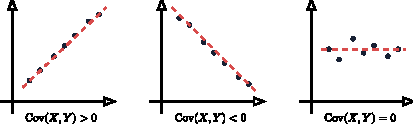
\includegraphics[keepaspectratio,alt={Three scatterplots with positive, negative, and zero linear covariance trends.}]{assets/fig-prob-02-random-variables-diagram-01.pdf}}
\caption{正、负与零协方差对应的线性趋势}\label{fig-prob-02-random-variables-diagram-01}
\end{figure}

但是注意:

\begin{itemize}
\item
  covariance 只捕捉 linear relationship, 即趋势是否呈直线, 不过不能捕捉 nonlinear relationship. 之后在学习 independence 的时候, 我们会知道即便 covariance 为 0, \(X\) 和 \(Y\) 仍然可能是 dependent 的. 比如, 如果 \((X,Y)\) 的联合分布 as a graph 是个圆圈, 那么 covariance 就是 0, 但显然这两个变量之间是有关系的.

  \begin{figure}
  \centering
  \pandocbounded{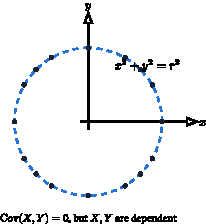
\includegraphics[keepaspectratio,alt={Points on a circle show dependent variables whose covariance is zero.}]{assets/fig-prob-02-random-variables-diagram-02.pdf}}
  \caption{零协方差但不独立的圆周分布}\label{fig-prob-02-random-variables-diagram-02}
  \end{figure}
\item
  Covariance 的数值还包括了这两个 random variables 的 scale, 因而还不能直接用来比较不同 random variables 之间的 linear relationship 的强弱程度. 真正公平的 linear relationship 还需要 normalize by norms, 把这个关系定位到 \(\lbrack - 1,1\rbrack\) 的区间上 即等下定义的 correlation.
\end{itemize}

\end{qlremark}

我们容易发现一件事情:

% qlnotes: kind=theorem; id=thm-02-random-variables-covariance-a-positive-semi-definite-symmetric-bilinear-f; concepts=covariance-a-positive-semi-definite-symmetric-bilinear-f; aliases=covariance 是一个 a positive semi-definite symmetric bilinear form
\begin{theorem}{covariance 是一个 a positive semi-definite symmetric bilinear form}\label{thm-02-random-variables-covariance-a-positive-semi-definite-symmetric-bilinear-f}

\begin{itemize}
\item
  covariance 是一个 \textbf{symmetric bilinear form} (并且 \textbf{translation-invariant}, 忽略 translation) 的 operator:

  \[\text{Cov}(aX + b,cY + d) = ac\,\text{Cov}(X,Y)\]\[\text{Cov}(X,Y) = \text{Cov}(Y,X)\]\[\text{Cov}(X + Y,Z) = \text{Cov}(X,Z) + \text{Cov}(Y,Z)\]
\item
  covariance 满足 positive definiteness: \(\text{Cov}(X,X) = \text{Var}(X) \geq 0\).
\end{itemize}

\end{theorem}

\begin{proof}

By def.

\end{proof}

而当我们把空间限定在 \(L_{0}^{2}(\Omega,\mathcal{F},{\mathbb{P}})\) 上时,

% qlnotes: kind=theorem; id=thm-02-random-variables-l-2-0-omega-mathcal-f-mathbb-p-hilbert-space-with-covar; concepts=l-2-0-omega-mathcal-f-mathbb-p-hilbert-space-with-covar; aliases=L^2_0(\Omega, \mathcal{F}, \mathbb{P}) 为一个 Hilbert space, with covariance as an inner product
\begin{theorem}{L\_\{0\}\^{}\{2\}(Omega,F,P) 为一个 Hilbert
space, with covariance as an inner product}\label{thm-02-random-variables-l-2-0-omega-mathcal-f-mathbb-p-hilbert-space-with-covar}

\(\ L_{0}^{2}(\Omega,\mathcal{F},{\mathbb{P}}),\langle \cdot , \cdot \rangle_{\text{Cov}}\ \) 为一个 Hilbert space, 即: covariance 在其上是一个 inner product (positive definite symmetric bilinear form).

\end{theorem}

\begin{proof}

很显然. 因为在 \(L^{2}\) space 上, 一个 constant random variable 的 variance 是 0, 但是它并不是一个零函数; 而在 \(L_{0}^{2}\) space 上, 所有的 random variables 都是 zero-centered 的, 因而 constant random variable 就是零函数了. 从而 covariance 在 \(L_{0}^{2}\) space 上是 positive definite 的, 从而是 inner product.\\

\end{proof}

而在 \(L_{0}^{2}(\Omega,\mathcal{F},{\mathbb{P}})\) 上, 两个 random variables \(X,Y\) 之间的夹角 \(\theta\) 的 cosine, 就是它们 真正的 linear relationship 的强弱程度, 因而我们把它叫做 correlation:

% qlnotes: kind=definition; id=def-02-random-variables-correlation; concepts=correlation; aliases=correlation
\begin{definition}{correlation}\label{def-02-random-variables-correlation}

\[\rho(X,Y) = \frac{\text{Cov}(X,Y)}{\sqrt{\text{Var}(X)}\sqrt{\text{Var}(Y)}}\]

\end{definition}

显然,

\[\rho(X,Y) = \cos\theta\]

where \(\theta\) 是 \(X,Y\) 之间的夹角. And we have:

\[\text{Cov}(X,Y) = \sigma_{X}\sigma_{Y}\rho(X,Y)\]

从而有以下显然的结论:

% qlnotes: kind=proposition; id=prop-02-random-variables-properties-of-correlation; concepts=properties-of-correlation; aliases=properties of correlation
\begin{proposition}{properties of correlation}\label{prop-02-random-variables-properties-of-correlation}

\begin{itemize}
\item
  \(\rho(X,Y) \in \lbrack - 1,1\rbrack\)
\item
  如果 \(\rho(X,Y) = 1\), 那么 \(Y = aX + b\) for some \(a > 0\) and \(b\); 如果 \(\rho(X,Y) = - 1\), 那么 \(Y = aX + b\) for some \(a < 0\) and \(b\).~
\item
  By Cauchy-Schwarz inequality, \(\left. |\text{Cov}(X,Y) \middle| \leq \sigma_{X}\sigma_{Y} \right.\).
\end{itemize}

\end{proposition}

做一个总结:

\begin{figure}
\centering
\caption{}
\end{figure}

\textbf{求两个 random variables 之间的 correlation, 就是把它们都 center 到 zero-centered 的位置 (即投影到 \(L_{0}^{2}\) space 上), 然后计算它们在 \(L_{0}^{2}\) space 上的 cosine similarity.}\\
此时我们看到 decomposition of variance:

% qlnotes: kind=proposition; id=prop-02-random-variables-random-variables-variance; concepts=-random-variables-variance; aliases=两个 random variables 之和的 variance
\begin{proposition}{两个 random variables 之和的 variance}\label{prop-02-random-variables-random-variables-variance}

两个 random variables 的和的 variance 可分解成 variances 和 covariance:

\[\text{Var}(X + Y) = \text{Var}(X) + \text{Var}(Y) + 2\ \text{Cov}(X,Y)\]

\end{proposition}

\begin{proof}

\[\text{Var}(X + Y) = {\mathbb{E}}\left\lbrack {(X + Y)^{2}} \right\rbrack - ({\mathbb{E}}\lbrack X + Y\rbrack)^{2} = {\mathbb{E}}\left\lbrack X^{2} \right\rbrack - ({\mathbb{E}}\lbrack X\rbrack)^{2} + {\mathbb{E}}\left\lbrack Y^{2} \right\rbrack - ({\mathbb{E}}\lbrack Y\rbrack)^{2} + 2({\mathbb{E}}\lbrack XY\rbrack - {\mathbb{E}}\lbrack X\rbrack{\mathbb{E}}\lbrack Y\rbrack)\]

\end{proof}

\begin{qlremark}{Remark}

它其实这就是标准的 inner product space 上的向量平方公式:

\[\parallel X + Y\underset{L_{0}^{2}}{\overset{2}{\parallel}} = \parallel X\underset{L_{0}^{2}}{\overset{2}{\parallel}} + \parallel Y\underset{L_{0}^{2}}{\overset{2}{\parallel}} + 2\langle X,Y\rangle_{L_{0}^{2}}\]

\end{qlremark}

\section{discrete random variables}\label{discrete-random-variables}

Recall: discrete random variable 是指其 range a.s. 是 countable 的 random variable. (存在一个 countable set \(S \subseteq {\mathbb{R}}\) 使得 \({\mathbb{P}}(X \in S) = 1\))

discrete RV 的 probability mass unction (pmf):

\[p_{X}(x) := {\mathbb{P}}(X = x),\quad\forall x \in {\mathbb{R}}\]

就是 \(X\) 的 distribution \(P^{X}\) 对于 counting measure of range \(S\) 的 Radon-Nikodym derivative:

\[p_{X} = \frac{d{\mathbb{P}}^{X}}{d\mu_{\text{S}}}\]

因为假设 \(X\) 的 range 是 \(S = \left\{ {x_{1},x_{2},\ldots} \right\}\), 那么对于任意 Borel set \(B\),

\[{\mathbb{P}}^{X}(B) = \sum\limits_{x_{i} \in B}{\mathbb{P}}(X = x_{i}) = \sum\limits_{x_{i} \in B \cap S}p_{X}(x_{i}) = \int_{A}p_{X}(x) d\mu_{\text{S}}(x)\]

下面我们给出一些经典的 discrete random variable 的例子, 以及它们的 pmf 和 cdf.

\subsection{Bernoulli distribution and Binomial distribution}\label{bernoulli-distribution-and-binomial-distribution}

% qlnotes: kind=example; id=ex-02-random-variables-bernoulli-distribution; concepts=bernoulli-distribution; aliases=(Bernoulli distribution)
\begin{example}[(Bernoulli distribution)]\label{ex-02-random-variables-bernoulli-distribution}

令 \(\Omega := \left\{ {\omega_{1},\omega_{2}} \right\}\), \(\mathcal{F} := 2^{\Omega}\).\\
令 \({\mathbb{P}}(\left\{ \omega_{1} \right\}) = p\), \({\mathbb{P}}(\left\{ \omega_{2} \right\}) = 1 - p\) 来表示这两个 singular 事件的概率.\\
令 \(X(\omega_{1}) = 1\), \(X(\omega_{2}) = 0\) 分别表示 success 和 failure.\\
那么显然可以计算:

\[{\mathbb{P}}(X = 0) = {\mathbb{P}}(\left\{ \omega_{2} \right\}) = 1 - p,\quad{\mathbb{P}}(X = 1) = {\mathbb{P}}(\left\{ \omega_{1} \right\}) = p\]

我们称 \((\Omega,\mathcal{F},{\mathbb{P}})\) 为一个 Bernoulli probability space (它 model 了一个 Bernoulli trial, 即一个 random experiment with two possible outcomes: success 和 failure)\\
称 \(X:\Omega\rightarrow\left\{ {0,1} \right\}\) 这个 random variable 为一个 \textbf{Bernoulli random variable}, 并称 \(X\) 的 distribution \(P^{X}\) 为一个 \textbf{Bernoulli distribution}, 写作

\[X \sim \text{Ber}(p)\]

这是最简单的 random variable 和 distribution 了. 它 model 的是: 比如我们 toss 一枚 biased coin, 以 \(p\) 的概率得到 heads (success), 以 \(1 - p\) 的概率得到 tails (failure).\\

\end{example}

% qlnotes: kind=proposition; id=prop-02-random-variables-proposition-010; concepts=proposition-010
\begin{proposition}\label{prop-02-random-variables-proposition-010}

如果 \(X \sim \text{Ber}(p)\), 那么 \({\mathbb{E}}\lbrack X\rbrack = p\), \(\text{Var}(X) = p(1 - p)\).

\end{proposition}

显然.

% qlnotes: kind=example; id=ex-02-random-variables-binomial-distribution; concepts=binomial-distribution; aliases=(Binomial distribution)
\begin{example}[(Binomial distribution)]\label{ex-02-random-variables-binomial-distribution}

我们 independently repeat \(n\) 次 Bernoulli trial, 每次 trial 的 success probability 都是 \(p\).\\
考虑:

\[S := X_{1} + X_{2} + \cdots + X_{n}\]

为 success 的总次数. 那么 \(S\) 是一个 discrete random variable \(S:\Omega^{n}\rightarrow{\mathbb{Z}}_{\geq 0}\) 容易计算出 \(S\) 的 pmf:

\[p_{S}(k) = {\mathbb{P}}(S = k) = \left( \frac{n}{k} \right)p^{k}(1 - p)^{n - k},\quad k = 0,1,\ldots,n\]

我们称 \(S\) 的 distribution \(P^{S}\) 为一个 \textbf{Binomial distribution}, 写作

\[S \sim \text{Bin}(n,p)\]

它 model 的是: 比如我们 toss 一枚 biased coin \(n\) 次, 得到 heads 的总次数.\\

\end{example}

% qlnotes: kind=proposition; id=prop-02-random-variables-proposition-011; concepts=proposition-011
\begin{proposition}\label{prop-02-random-variables-proposition-011}

如果 \(S \sim \text{Bin}(n,p)\), 那么 \({\mathbb{E}}\lbrack S\rbrack = np\), \(\text{Var}(S) = np(1 - p)\).

\end{proposition}

\begin{proof}

\[{\mathbb{E}}\lbrack X\rbrack = \sum\limits_{k = 1}^{n}k \cdot {\mathbb{P}}(X = k) = \sum\limits_{k = 1}^{n}k \cdot \left( \frac{n}{k} \right)p^{k}(1 - p)^{n - k} = p(1 - p)^{n - 1}\sum\limits_{k = 1}^{n}k \cdot \left( \frac{n}{k} \right)(\frac{p}{1 - p})^{k - 1}\]

由于

\[(1 + t)^{n} = \sum\limits_{k = 0}^{n}\left( \frac{n}{k} \right)t^{k}\Longrightarrow n(1 + t)^{n - 1} = \sum\limits_{k = 1}^{n}k \cdot \left( \frac{n}{k} \right)t^{k - 1}\]

可以得到

\[{\mathbb{E}}\lbrack X\rbrack = p(1 - p)^{n - 1} \cdot n(1 + \frac{p}{1 - p})^{n - 1} = np\]

然后计算得 \(\text{Var}(X) = np(1 - p)\). 但是这是比较麻烦的方法. 也可以利用 \(X = \sum_{i = 1}^{n}X_{i}\), 其中 \(X_{i} \sim \text{Ber}(p)\) i.i.d 这个事实来计算, 那么直接通过 线性叠加 Bernoulli random variable 的 expectation 和 variance 就可以了.

\end{proof}

\subsection{Geometric distribution and Negative Binomial distribution}\label{geometric-distribution-and-negative-binomial-distribution}

% qlnotes: kind=example; id=ex-02-random-variables-geometric-distribution; concepts=geometric-distribution; aliases=(Geometric distribution)
\begin{example}[(Geometric distribution)]\label{ex-02-random-variables-geometric-distribution}

我们 perform independent Bernoulli trial, 每次 trial 的 success probability 都是 \(p\).\\
考虑 random variable \(T\) 表示第一次 success 发生的 trial number. (也就是等于: 我们一直 trial, 直到第一次 success 发生, 那么这个 trial 的 number 就是 \(T\)).\\
那么 \(T\) 是一个 discrete random variable \(T:\Omega^{\infty}\rightarrow{\mathbb{Z}}_{\geq 1}\).\\
容易计算出 \(T\) 的 pmf:

\[p_{T}(k) = {\mathbb{P}}(T = k) = (1 - p)^{k - 1}p,\quad k = 1,2,\ldots\]

我们称 \(T\) 的 distribution \(P^{T}\) 为一个 \textbf{Geometric distribution}, 写作

\[T \sim \text{Geom}(p)\]

它 model 的是: 比如我们 toss 一枚 biased coin, 第一次得到 heads 的 trial number.\\

\end{example}

% qlnotes: kind=proposition; id=prop-02-random-variables-proposition-012; concepts=proposition-012
\begin{proposition}\label{prop-02-random-variables-proposition-012}

如果 \(X \sim \text{Geom}(p)\), 那么 \({\mathbb{E}}\lbrack X\rbrack = 1/p\), \(\text{Var}(X) = (1 - p)/p^{2}\).

\end{proposition}

\begin{proof}

\[{\mathbb{E}}\lbrack X\rbrack = \sum\limits_{k = 1}^{\infty}k(1 - p)^{k - 1}p = p\sum\limits_{k = 1}^{\infty}k(1 - p)^{k - 1} = p\  - \frac{d}{d(1 - p)}\sum\limits_{k = 0}^{\infty}(1 - p)^{k} = - p - \frac{d}{dp}\frac{1}{1 - (1 - p)} = \frac{1}{p}\]

similarly, 可以计算得

\[{\mathbb{E}}\lbrack X^{2}\rbrack = \frac{2 - p}{p^{2}}\]

因而

\[\text{Var}\lbrack X\rbrack = {\mathbb{E}}\lbrack X^{2}\rbrack - ({\mathbb{E}}\lbrack X\rbrack)^{2} = \frac{1 - p}{p^{2}}\]

\end{proof}

% qlnotes: kind=example; id=ex-02-random-variables-negative-binomial-distribution; concepts=negative-binomial-distribution; aliases=(Negative Binomial distribution)
\begin{example}[(Negative Binomial distribution)]\label{ex-02-random-variables-negative-binomial-distribution}

这是 Geometric distribution 的 generalization (但不完全一样).\\
我们 perform independent Bernoulli trial, 每次 trial 的 success probability 都是 \(p\). (即 independent and identically distributed)\\
令 random variable \(T_{r}\) 表示第 \(r\) 次 success 发生之前 的 failures 的数量. (也就是等于: 我们一直 trial, 直到第 \(r\) 次 success 发生, 那么这个 trial 的 number 就是 \(T_{r} + r\), 因为 \(T_{r}\) 是 failures 的数量, 还要加上 \(r - 1\) 个 success. ).\\
那么 \(T_{r}\) 是一个 discrete random variable \(T_{r}:\Omega^{\infty}\rightarrow{\mathbb{Z}}_{\geq 0}\).\\
容易计算出 \(T_{r}\) 的 pmf:

\[p_{T_{r}}(k) = {\mathbb{P}}(T_{r} = k) = \left( \frac{k + r - 1}{k} \right)(1 - p)^{k}p^{r},\quad k = 0,1,2,\ldots\]

这是因为:最后一次 success 的位置是固定的. 我们要在前 \(k + r - 1\) 次 trial 中选择 \(k\) 次作为 failures.\\
我们称 \(T_{r}\) 的 distribution \(P^{T_{r}}\) 为一个 \textbf{Negative Binomial distribution}, 写作

\[T_{r} \sim \text{NB}(r,p)\]

它 model 的是: 比如我们 toss 一枚 biased coin, 得到第 \(r\) 个 heads 之前会经历的 failures 的数量.\\

\end{example}

\subsection{Poisson distribution}\label{poisson-distribution}

% qlnotes: kind=example; id=ex-02-random-variables-poisson-distribution; concepts=poisson-distribution; aliases=(Poisson distribution)
\begin{example}[(Poisson distribution)]\label{ex-02-random-variables-poisson-distribution}

考虑这一 pmf:

\[{\mathbb{P}}(X = k) = e^{- \lambda}\frac{\lambda^{k}}{k!},\quad k = 0,1,2,\ldots\]

我们称 \(X\) 的 distribution \(P^{X}\) 为一个 \textbf{Poisson distribution}, 写作

\[X \sim \text{Poi}(\lambda),\quad\lambda > 0\]

以 \(\lambda = 3\) 为例画出 pmf 示意图:

\begin{figure}
\centering
\pandocbounded{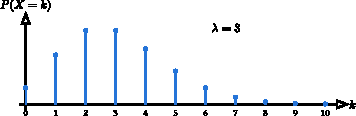
\includegraphics[keepaspectratio,alt={A stem plot of the Poisson probability mass function with lambda equal to 3.}]{assets/fig-prob-02-random-variables-diagram-03.pdf}}
\caption{参数 \(\lambda = 3\) 的 Poisson 概率质量函数}\label{fig-prob-02-random-variables-diagram-03}
\end{figure}

\begin{qlremark}{Remark}

当 \(n\rightarrow\infty\) 时, \(\text{Bin}(n,\lambda/n)\) 的 distribution 趋近于 \(\text{Poi}(\lambda)\).\\
考虑 \(X \sim B\left( {n,\frac{\lambda}{n}} \right)\), 对于固定的 \(k\):

\[{\mathbb{P}}(X = k) = \left( \frac{n}{k} \right)\left( \frac{\lambda}{n} \right)^{k}\left( {1 - \frac{\lambda}{n}} \right)^{n - k}\]

展开组合数 \(\left( \frac{n}{k} \right)\):

\[{\mathbb{P}}(X = k) = \frac{n(n - 1)\ldots(n - k + 1)}{k!} \cdot \frac{\lambda^{k}}{n^{k}} \cdot \left( {1 - \frac{\lambda}{n}} \right)^{n} \cdot \left( {1 - \frac{\lambda}{n}} \right)^{- k}\]

重组项:

\[{\mathbb{P}}(X = k) = \frac{\lambda^{k}}{k!} \cdot \underset{(1)}{\underbrace{\frac{n(n-1)\ldots(n-k+1)}{n^{k}}}} \cdot \underset{(2)}{\underbrace{\left( {1-\frac{\lambda}{n}} \right)^{n}}} \cdot \underset{(3)}{\underbrace{\left( {1-\frac{\lambda}{n}} \right)^{-k}}}\]

其中, (1) 的 limit 是 1, (2) 的 limit 是 \(e^{- \lambda}\), (3) 的 limit 是 1, 因而

\[\lim\limits_{n\rightarrow\infty}{\mathbb{P}}(X = k) = e^{- \lambda}\frac{\lambda^{k}}{k!}\]

这个极限行为的意义是:

\begin{itemize}
\item
  \(\lambda\) 表示: 在一个固定时间/空间窗口内, 一个事件出现的平均次数的观测.
\item
  我们把这段时间间分成 \(n\) 个小窗口, 将这个观测作为先验知识用来 model 这类事件实现的平均概率, 那么 每个小窗口内事件出现的概率是 \(p = \lambda/n\).
\item
  每个 \(\text{Bin}(n,\lambda/n)\) 都表示: 在时间细分成 \(n\) 个小窗口的情况下, 这个事件出现的次数的分布. (注意不是在时间上的分布, 而是在次数上的分布)
\item
  当 \(n\rightarrow\infty\) 时, 其意义: 基于连续时间的估计, 这个事件在原固定事件窗口内出现的次数的分布. 这就是 \(\text{Poi}(\lambda)\) 的意义.
\end{itemize}

因而 Poisson distribution 的意义本质上是: \textbf{给定对一个事件在固定窗口下出现的平均次数的观测(估计), 那么这个事件在这个窗口内出现 \(n\) 次 (\(n = 0,1,2,\cdots\))的概率是多少?}\\
所以 Poisson 分布, 即是\textbf{根据一个事件在给定 windows 内发生次数的 expectation, 来估计这个事件在该 windows 内发生次数的分布的标准方法.}\\

\end{qlremark}

\begin{qlremark}{Remark}

Further remark: Poisson distribution 的用途.

\begin{itemize}
\item
  它是 model "大量级的小概率事件" 的通用模型.\\
  即一段时间内, 一件事情的发生的概率非常小 (\(p \ll 1\)), 但是有很多机会发生 (\(n \gg 1\)). 比如放射性衰变.
\item
  现实世界中, 对于一些事情, 我们想要 model 其在一段时间内发生的总次数 (\(n\)) 和单次成功率 (\(p\)) 是很困难的. 比如统计今天路过百货大楼的总人数 (\(n\)), 以及每个人路过百货大楼时走进去的概率 (\(p\)). 但是我们 很容易可以知道: \(\lambda = np\) 的观测. 即: 每天平均有多少人走进百货大楼. 那么我们就可以用 Poisson distribution 来 model 这件事情在一天内发生的次数的分布.\\
\end{itemize}

\end{qlremark}

\end{example}

% qlnotes: kind=proposition; id=prop-02-random-variables-proposition-013; concepts=proposition-013
\begin{proposition}\label{prop-02-random-variables-proposition-013}

如果 \(X \sim \text{Poi}(\lambda)\), 那么 \({\mathbb{E}}\lbrack X\rbrack = \lambda\), \(\text{Var}(X) = \lambda\).

\end{proposition}

\begin{proof}

recall \(e^{x}\) 的 taylor expansion:

\[e^{x} = \sum\limits_{k = 0}^{\infty}\frac{x^{k}}{k!}\]

因而

\[{\mathbb{E}}\lbrack X\rbrack = \sum\limits_{k = 0}^{\infty}ke^{- \lambda}\frac{\lambda^{k}}{k!} = e^{- \lambda}\lambda\sum\limits_{k = 1}^{\infty}\frac{\lambda^{k - 1}}{(k - 1)!} = e^{- \lambda}\lambda e^{\lambda} = \lambda\]

similarly, 可以计算得

\[{\mathbb{E}}\lbrack X^{2}\rbrack = \lambda^{2} + \lambda\]

因此,

\[\text{Var}(X) = {\mathbb{E}}\lbrack X^{2}\rbrack - ({\mathbb{E}}\lbrack X\rbrack)^{2} = \lambda\]

\end{proof}

\subsubsection{Poisson distribution 的 additivity}\label{poisson-distribution-ux7684-additivity}

% qlnotes: kind=theorem; id=thm-02-random-variables-additivity-of-poisson-distribution; concepts=additivity-of-poisson-distribution; aliases=additivity of Poisson distribution
\begin{theorem}{additivity of Poisson distribution}\label{thm-02-random-variables-additivity-of-poisson-distribution}

如果 \(X \sim \text{Poi}(\lambda_{1})\), \(Y \sim \text{Poi}(\lambda_{2})\) are independent, 那么

\[X + Y \sim \text{Poi}(\lambda_{1} + \lambda_{2})\]

\end{theorem}

\begin{qlremark}{Remark}

这个事实通过简单的计算即可得到.

但是值得一提的是, 我们之后会证明一个结论: 两个 independent 的 random variable 的 sum 的 distribution 是它们 convolution 的 distribution.

而 Poisson distribution 的 convolution 仍然是 Poisson distribution, 并且是 linear 的. 这就是 additivity of Poisson distribution 的本质原因.

\end{qlremark}

\section{continuous random variables}\label{continuous-random-variables}

recall: 总而言之, continuous random variable 是指其 distribution \({\mathbb{P}}^{X}\) 对于 Lebesgue measure \(m\) 是 absolutely continuous 的 random variable, 等价于存在一个 pdf \(f_{X}\) 使得

\[F_{X}(x) = \int_{- \infty}^{x}f_{X}(y)dy\]

对于任意 \(x\) 都成立.

而由 \({\mathbb{E}}\lbrack X\rbrack = \int_{\Omega}Xd{\mathbb{P}} = \int_{\mathbb{R}}xd{\mathbb{P}}^{X} = \int_{\mathbb{R}}xf_{X}(x)dx\) 可得

\[{\mathbb{E}}\lbrack X\rbrack = \int_{- \infty}^{+ \infty}xf_{X}(x)dx,\quad\text{Var}(X) = \int_{- \infty}^{+ \infty}(x - {\mathbb{E}}\lbrack X\rbrack)^{2}f_{X}(x)dx\]

这里还有一个额外的结论:

% qlnotes: kind=proposition; id=prop-02-random-variables-proposition-014; concepts=proposition-014
\begin{proposition}\label{prop-02-random-variables-proposition-014}

对于任意的 measurable function \(g:{\mathbb{R}}\rightarrow{\mathbb{R}}\), 都有

\[{\mathbb{E}}\lbrack g(X)\rbrack = \int_{- \infty}^{+ \infty}g(x)f_{X}(x)dx\]

\end{proposition}

\begin{proof}

\[\begin{matrix}
{{\mathbb{E}}\lbrack g(X)\rbrack} & {= \int_{\Omega}g(X(w))\, d{\mathbb{P}}(w)} \\
 & {= \int_{\Omega}g \circ X\, d{\mathbb{P}}} \\
 & {= \int_{\mathbb{R}}g\, d{\mathbb{P}}^{X}} \\
 & {= \int_{- \infty}^{+ \infty}g(x)f_{X}(x)\, dx}
\end{matrix}\]

\end{proof}

下面我们介绍一些常见的 continuous random variables, 以及它们的 pdf, cdf, expectation 和 variance.

\subsection{uniform distribution: 最简单的 continuous RV}\label{uniform-distribution-ux6700ux7b80ux5355ux7684-continuous-rv}

% qlnotes: kind=definition; id=def-02-random-variables-uniform-distribution; concepts=uniform-distribution; aliases=uniform distribution
\begin{definition}{uniform distribution}\label{def-02-random-variables-uniform-distribution}

如果 \(f_{X}(x) = \frac{1}{b - a}\) on \((a,b)\) and \(0\) elsewhere, 那么我们称 \(X\) 的 distribution \(P^{X}\) 为一个 \textbf{uniform distribution}, 写作

\[X \sim U(\lbrack a,b\rbrack)\]

\end{definition}

对于 uniform distribution, 很容易计算得:

\[F_{X}(x) = \frac{x - b}{b - a},\quad{\mathbb{E}}\lbrack X\rbrack = \frac{a + b}{2},\quad\text{Var}(X) = \frac{(b - a)^{2}}{12}\]

% qlnotes: kind=example; id=ex-02-random-variables-uniform-distribution-pdf-cdf; concepts=uniform-distribution-pdf-cdf; aliases=(uniform distribution 的 pdf 和 cdf)
\begin{example}[(uniform distribution 的 pdf 和 cdf)]\label{ex-02-random-variables-uniform-distribution-pdf-cdf}

考虑 \(X \sim U(\lbrack a,b\rbrack)\), 其 pdf 和 cdf 的图像如下:

\begin{figure}
\centering
\pandocbounded{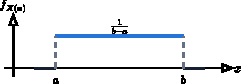
\includegraphics[keepaspectratio,alt={The uniform density is constant at 1/(b-a) between a and b and zero outside.}]{assets/fig-prob-02-random-variables-diagram-04.pdf}}
\caption{区间 \(\left\lbrack {a,b} \right\rbrack\) 上均匀分布的概率密度函数}\label{fig-prob-02-random-variables-diagram-04}
\end{figure}

\begin{figure}
\centering
\pandocbounded{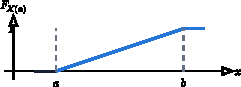
\includegraphics[keepaspectratio,alt={The uniform cumulative distribution rises linearly from zero at a to one at b.}]{assets/fig-prob-02-random-variables-diagram-05.pdf}}
\caption{区间 \(\left\lbrack {a,b} \right\rbrack\) 上均匀分布的累积分布函数}\label{fig-prob-02-random-variables-diagram-05}
\end{figure}

\end{example}

\subsection{exponential distribution: geometric distribution 的 continuous version}\label{exponential-distribution-geometric-distribution-ux7684-continuous-version}

Exponential random variable model 的是一盏灯的 remaining lifetime. 它 assume: 任意时间, 这盏灯有一个 constant 的磨损速率.

假设它的磨损速率是 \(\lambda = \lambda_{X}(t)\) for all \(t\), 那么在任意时间 \(t\) 上:

\[\lambda_{X}(t) = \lim\limits_{h\rightarrow 0^{+}}\frac{P(X \in (t,t + h\rbrack)}{h} = \lim\limits_{h\rightarrow 0^{+}}\frac{{\mathbb{P}}(t \leq X \leq t + h)}{h} \cdot \frac{1}{{\mathbb{P}}(X > t)} = \frac{f_{X}(t)}{1 - F_{X}(t)}\]

即 ODE:

\[\lambda = \frac{F_{X}'(t)}{1 - F_{X}(t)}\]

with initial condition \(F_{X}(0) = 0\).

我们知道这个 ODE 的 solution 是:

\[\begin{matrix}
{F_{X}(t) = \{ 1 - e^{- \lambda t},\quad t > 0} \\
{0,\quad t \leq 0,\quad f_{X}(t) = \{\lambda e^{- \lambda t},\quad t > 0} \\
{0,\quad t \leq 0}
\end{matrix}\]

% qlnotes: kind=definition; id=def-02-random-variables-exponential-distribution; concepts=exponential-distribution; aliases=exponential distribution
\begin{definition}{exponential distribution}\label{def-02-random-variables-exponential-distribution}

我们称 \(X\) 为一个 \textbf{exponential random variable} with parameter \(\lambda\), 如果它的 pdf is given by:

\[\begin{matrix}
{f(x) = \{\lambda e^{- \lambda x},\quad x > 0} \\
{0,\quad x \leq 0}
\end{matrix}\]

写作

\[X \sim \text{Exp}(\lambda)\]

\end{definition}

刚才已经计算出, exponential random variable 的 distribution 为

\[\begin{matrix}
{F_{X}(x) = \{\int_{- \infty}^{x}f(t) dt = \lambda\int_{0}^{x}e^{- \lambda t} dt = 1 - e^{- \lambda x},\quad x > 0} \\
{0,\quad x < 0}
\end{matrix}\]

容易验证, \(F_{X}(x) = 0\) when \(x\rightarrow - \infty\), 以及 \(F_{X}(x)\rightarrow 1\) when \(x\rightarrow\infty\)

计算其 expectation:

\[\begin{matrix}
{{\mathbb{E}}\lbrack X^{n}\rbrack} & {= \lambda\int_{0}^{\infty}x^{n}e^{- \lambda x} dx} \\
 & {= - \int_{0}^{\infty}x^{n}(e^{- \lambda x})' dx} \\
 & {= 0 + \int_{0}^{\infty}nx^{n - 1}e^{- \lambda x} dx} \\
 & {= \frac{n}{\lambda}{\mathbb{E}}(X^{n - 1})}
\end{matrix}\]

并 notice: \({\mathbb{E}}\lbrack X^{0}\rbrack = {\mathbb{E}}\lbrack 1\rbrack = 1\). 因而 recursively get:

\[{\mathbb{E}}\lbrack X^{n}\rbrack = \frac{n!}{\lambda^{n}}\]

即: \({\mathbb{E}}\lbrack X\rbrack = \frac{1}{\lambda},{\mathbb{E}}\lbrack X^{2}\rbrack = \frac{2}{\lambda^{2}},\cdots\) 从而:

\[Var\lbrack X\rbrack = \frac{2}{\lambda^{2}} - \frac{1}{\lambda^{2}} = \frac{1}{\lambda^{2}}\]

\begin{figure}
\centering
\pandocbounded{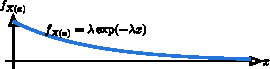
\includegraphics[keepaspectratio,alt={The exponential density decreases from lambda toward zero as x increases.}]{assets/fig-prob-02-random-variables-diagram-06.pdf}}
\caption{指数分布的概率密度函数}\label{fig-prob-02-random-variables-diagram-06}
\end{figure}

\begin{figure}
\centering
\pandocbounded{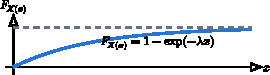
\includegraphics[keepaspectratio,alt={The exponential cumulative distribution rises from zero toward one.}]{assets/fig-prob-02-random-variables-diagram-07.pdf}}
\caption{指数分布的累积分布函数}\label{fig-prob-02-random-variables-diagram-07}
\end{figure}

\begin{qlremark}{Remark}

exponential 随机变量是 geometric 随机变量的 continuous analogue. 因为 geometric random variable 是假设一个事件在 每个时间点以 constant 的概率发生, 用来 model 它第一次发生的时间;

而 exponential random variable 其实也是, 只是 on a continuous time scale: 它假设的 constant 损坏率其实 implies: \textbf{在任意时间, 如果灯还没坏, 那么灯此刻坏掉的概率是 constant 的.}

% qlnotes: kind=theorem; id=thm-02-random-variables-memoryless-property-of-exponential-distribution; concepts=memoryless-property-of-exponential-distribution; aliases=memoryless property of exponential distribution
\begin{theorem}{memoryless property of exponential distribution}\label{thm-02-random-variables-memoryless-property-of-exponential-distribution}

任意 continuous RV,

\[{\mathbb{P}}(X > b + t \mid X > b) = {\mathbb{P}}(X > t)\Leftrightarrow X\ \text{is an exponential random variable}\]

\end{theorem}

\begin{proof}

简单而言

\[\begin{matrix}
 & {P(X > b + t \mid X > b) = P(X > t)} \\
\Leftrightarrow & {P(X > b + t) = P(X > t)P(X > b)} \\
\Leftrightarrow & {X\ \text{exponential}}
\end{matrix}\]

\end{proof}

因而对于 geometric RV 的 pmf, 当我们把时间间隔 (discrete time interval) 变得越来越小, 这一行为的极限就变为了 exponential RV 的 pdf.

这是一个很自然的 limit behavior, 此处不验证了.

\end{qlremark}

% qlnotes: kind=example; id=ex-02-random-variables-example-011; concepts=example-011
\begin{example}\label{ex-02-random-variables-example-011}

假设我们有一个 storage battery, 它的 lifetime 是 exponentially distributed 的, 并且 average 为 10 hours. Suppose 我们想要 use this battery for 5 hours for.

计算: probability of finishing the task, if:\\
(a) 使用一个 new battery\\
(b) 使用一个已经用过 2 hours 的 battery\\

\end{example}

\begin{qlsolution}{Solution}

\[{\mathbb{E}}\lbrack X\rbrack = 10 = \frac{1}{\lambda}\Longrightarrow\lambda = \frac{1}{10}\]

如果我们使用一个 new battery, 则 want: \(P(X > 5) = 1 - P(X < 5) = 1 - F_{X}(5) = e^{- \frac{1}{2}}\) 如果我们使用一个用过 2 hours 的 battery, 则 want:

\[P(X > 5 + 2 \mid X > 2) = \frac{e^{- (5 + 2)\lambda}}{e^{- 2\lambda}} = e^{- 5\lambda} = = e^{- \frac{1}{2}}\]

Notice:

\[P(X > 5) = P(X > 5 + 2 \mid X > 2)\]

\end{qlsolution}

\subsection{Gamma distribution: negative binomial distribution 的 continuous version}\label{gamma-distribution-negative-binomial-distribution-ux7684-continuous-version}

recall Gamma 函数:

\[\Gamma(\alpha) = \int_{0}^{\infty}x^{\alpha - 1}e^{- x} dx\]

这个函数有一个重要的性质:

\[\Gamma(\alpha + 1) = \alpha\Gamma(\alpha)\]

因而对于 \(n \in {\mathbb{N}}\), 我们有:

\[\Gamma(n) = (n - 1)!\]

Gamma 函数就是 factorial 函数的 continuous generalization.

% qlnotes: kind=definition; id=def-02-random-variables-gamma-distribution; concepts=gamma-distribution; aliases=\Gamma-distribution
\begin{definition}{Gamma-distribution}\label{def-02-random-variables-gamma-distribution}

如果 continuous random variable \(X\) 的 pdf 是:

\[f_{X}(x) = \left\{ \begin{matrix}
{\frac{\lambda^{\alpha}}{\Gamma(\alpha)}x^{\alpha - 1}e^{- \lambda x},} & {x > 0,} \\
{0,} & {x \leq 0}
\end{matrix} \right.\]

那么我们称 \(X\) 服从 \textbf{\(\Gamma\) distribution}, 写作

\[X \sim \Gamma(\alpha,\lambda)\]

其中 \(\alpha > 0\) 称为 shape parameter, \(\lambda > 0\) 称为 rate parameter.

\end{definition}

\(\Gamma\) distribution 的 cdf 这样求: for \(a \geq 0\),

\[\begin{matrix}
{F_{X}(a) = \int_{- \infty}^{a}f_{X}(x) dx} & {= \int_{0}^{a}\frac{\lambda^{\alpha}}{\Gamma(\alpha)}x^{\alpha - 1}e^{- \lambda x} dx} \\
 & {= \frac{1}{\Gamma(\alpha)}\int_{0}^{\lambda a}t^{\alpha - 1}e^{- t} dt}
\end{matrix}\]

and for \(a < 0\), \(F_{X}(a) = 0\).

Expectation:

\[\begin{matrix}
{{\mathbb{E}}\lbrack X\rbrack} & {= \frac{1}{\Gamma(\alpha)}\int_{0}^{\infty}(\lambda x)^{\alpha - 1}\lambda e^{- \lambda x} dx} \\
 & {= \frac{1}{\lambda\Gamma(\alpha)}\int_{0}^{\infty}x^{\alpha}e^{- x} dx} \\
 & {= \frac{\Gamma(\alpha + 1)}{\lambda\Gamma(\alpha)} = \frac{\alpha}{\lambda}}
\end{matrix}\]

(since \(\Gamma(\alpha + 1) = \alpha\Gamma(\alpha)\).) 同理我们可以计算得: \({\mathbb{E}}\lbrack X^{2}\rbrack = \frac{\alpha(\alpha + 1)}{\lambda^{2}}\) 从而

\[\text{Var}\lbrack X\rbrack = {\mathbb{E}}\lbrack X^{2}\rbrack - ({\mathbb{E}}\lbrack X\rbrack)^{2} = \frac{\alpha(\alpha + 1)}{\lambda^{2}} - \frac{\alpha^{2}}{\lambda^{2}} = \frac{\alpha}{\lambda^{2}}\]

容易发现: 当 \(\alpha = 1\) 时, \(\Gamma\) distribution 就退化成了 exponential distribution.

\[\Gamma(1,\lambda) = \text{Exp}(\lambda)\]

而当 \(\alpha\) 是一个正整数 \(n\) 时, \(\Gamma\) distribution 实际就是 \(n\) 个 independent exponential distribution 的 sum:

% qlnotes: kind=proposition; id=prop-02-random-variables-gamma-distribution-independent-exponential-distribution-su; concepts=gamma-distribution-independent-exponential-distribution-su; aliases=Gamma distribution 即是 independent exponential distribution 的 sum
\begin{proposition}{Gamma distribution 即是 independent exponential distribution 的 sum}\label{prop-02-random-variables-gamma-distribution-independent-exponential-distribution-su}

Let \(X_{1},X_{2},\cdots,X_{n} \sim \text{Exp}(\lambda)\) be i.i.d., 则

\[\Gamma(n,\lambda) = \sum\limits_{i = 1}^{n}X_{i}\]

\end{proposition}

\begin{proof}

证明这一结论除了硬算之外, 更快的方法是通过 moment generating function. //TODO

\end{proof}

\begin{qlremark}{Remark}

Gamma distribution 即多个 i.i.d. exponential distribution 的 sum; 而我们知道 exponential distribution 是 geometric distribution 的 continuous analogue; 因而 \textbf{Gamma distribution 也是 negative binomial distribution 的 continuous analogue.}

考虑固定 rate parameter \(\lambda = 1\)，不同 shape parameter \(\alpha\) 的 Gamma distribution：

\begin{figure}
\centering
\pandocbounded{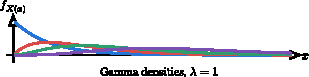
\includegraphics[keepaspectratio,alt={Gamma density curves for alpha 1, 2, 3, and 5 with lambda fixed at 1.}]{assets/fig-prob-02-random-variables-diagram-08.pdf}}
\caption{固定 \(\lambda = 1\) 时不同 shape 参数的 Gamma 密度}\label{fig-prob-02-random-variables-diagram-08}
\end{figure}

\begin{figure}
\centering
\pandocbounded{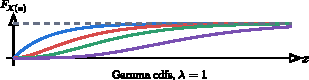
\includegraphics[keepaspectratio,alt={Gamma cumulative distribution curves for alpha 1, 2, 3, and 5 with lambda fixed at 1.}]{assets/fig-prob-02-random-variables-diagram-09.pdf}}
\caption{固定 \(\lambda = 1\) 时不同 shape 参数的 Gamma 分布函数}\label{fig-prob-02-random-variables-diagram-09}
\end{figure}

\begin{itemize}
\item
  当 \(\alpha = 1\) 时, Gamma 分布退化为指数分布, pdf 单调递减;
\item
  随着 \(\alpha\) 增大, pdf 从 0 处开始上升, 形成驼峰形状, 并逐渐向右平移;
\item
  cdf 随 \(\alpha\) 增大而上升变缓, 表示分布的右尾变长。
\end{itemize}

\end{qlremark}

\subsection{normal random variables: 最重要的 continuous RV, 任意 RV 的叠加极限}\label{normal-random-variables-ux6700ux91cdux8981ux7684-continuous-rv-ux4efbux610f-rv-ux7684ux53e0ux52a0ux6781ux9650}

% qlnotes: kind=definition; id=def-02-random-variables-definition-017; concepts=definition-017
\begin{definition}\label{def-02-random-variables-definition-017}

我们称 \(X\) is \textbf{normally distributed with parameter \(\mu\) and \(\sigma\)}, if the pdf of \(X\) is given by:

\[p(x) = \frac{1}{\sigma\sqrt{2\pi}}e^{- \frac{(x - \mu)^{2}}{2\sigma^{2}}}\]

写作:

\[X \sim \mathcal{N}(\mu,\sigma^{2})\]

特别地, 当 \(\mu = 0,\sigma = 1\) 时,

\[X \sim \mathcal{N}(0,1)\]

被称为 \textbf{standard normal distribution.}

\end{definition}

\begin{itemize}
\item
  验证其为 valid pdf:

  我们首先验证 standard normal distribution. 令:

  \[I := \int_{0}^{\infty}e^{\frac{- y^{2}}{2}} dy\]

  则

  {𝐼2=∫0∞𝑒−𝑦22𝑑𝑦⋅∫0∞𝑒−𝑥22𝑑𝑥=∫ℝ≥02𝑒−𝑥2+𝑦22𝑑𝑥𝑑𝑦=∫0𝜋/2∫0∞𝑒−𝑟22𝑟𝑑𝑟𝑑𝜃=∫0𝜋/2−𝑒−𝑟220∞𝑑𝜃=∫0𝜋/21𝑑𝜃=𝜋2}

  从而得到 \(I = \frac{\sqrt{2\pi}}{2}\). 因而 \(\int_{- \infty}^{\infty}e^{- \frac{x^{2}}{2}}\, dx = \sqrt{2\pi}\), 因而 \(\int_{\mathbb{R}}p(x)\, dx = 1\).

  从而对于任意的 \(\mu\) 和 \(\sigma\), 通过 change of variable formula 易得 \(\int_{\mathbb{R}}p(x)\, dx = 1\).
\item
  计算其 expectation 和 variance:

  我们只需要计算 standard normal distribution 的 expectation 和 variance, 然后通过 expectation 的 linearity 和 variance 的 scale invariance 来计算.

  令 \(X \sim \mathcal{N}(0,1)\). Then

  \[{\mathbb{E}}\lbrack X\rbrack = \frac{1}{\sqrt{2\pi}}\int_{\mathbb{R}}xe^{- \frac{x^{2}}{2}} dx = 0\]

  因为这是一个 \textbf{odd function}. 从而

  {𝔼{[}𝑋2{]}=12𝜋∫ℝ𝑥2𝑒−𝑥22𝑑𝑥=12𝜋∫ℝ𝑥(𝑥𝑒−𝑥22)𝑑𝑥=12𝜋∫ℝ𝑥(𝑒−𝑥22)′𝑑𝑥=−12𝜋𝑥𝑒−𝑥22−∞∞+12𝜋∫ℝ𝑒−𝑥22𝑑𝑥=0+1=1}

  从而:

  \[\text{Var}(X) = 1\]

  For general normally distributed \(Y\), 我们知道了 \(X: = \frac{Y - \mu}{\sigma}\) 的 \({\mathbb{E}}\lbrack X\rbrack = 0\), \(\text{Var}(X) = 1\), 因而

  \[{\mathbb{E}}\lbrack Y\rbrack = {\mathbb{E}}\lbrack\sigma X + \mu\rbrack = \mu\]

  and

  \[\text{Var}(Y) = \text{Var}(\sigma X + \mu) = {\mathbb{E}}\lbrack(\sigma X + \mu - \mu)^{2}\rbrack = {\mathbb{E}}(\sigma^{2}X^{2}) = \sigma^{2}{\mathbb{E}}\lbrack X^{2}\rbrack = \sigma^{2}\]

  对于多个 i.i.d. normally distributed \(X\),

  \[{\mathbb{E}}\lbrack X^{k}\rbrack = \frac{1}{\sqrt{2\pi}}\int_{\mathbb{R}}x^{k}e^{- \frac{x^{2}}{2}} dx\]

  For \(k\) odd, it is \(0\).\\
  For \(k\) even:

  \[\begin{matrix}
  {{\mathbb{E}}\lbrack X^{k}\rbrack} & {= \frac{1}{\sqrt{2\pi}}\int_{\mathbb{R}}x^{k - 1}(xe^{- \frac{x^{2}}{2}}) dx} \\
   & {= - \frac{1}{\sqrt{2\pi}}\int_{\mathbb{R}}x^{k - 1}(e^{- \frac{x^{2}}{2}})' dx} \\
   & {= 0 + \frac{1}{\sqrt{2\pi}}\int_{\mathbb{R}}(x^{k - 1})'e^{- \frac{x^{2}}{2}} dx} \\
   & {= \frac{k - 1}{\sqrt{2\pi}}\int_{\mathbb{R}}x^{k - 2}e^{- \frac{x^{2}}{2}} dx} \\
   & {= (k - 1){\mathbb{E}}\lbrack X^{k - 2}\rbrack}
  \end{matrix}\]

  从而:

  \[\begin{matrix}
  {{\mathbb{E}}\lbrack X^{k}\rbrack = \{ 0,\quad k = 2j - 1} \\
  {(2j - 1)(2j - 3)\cdots 1 = \frac{(2j)!}{2^{j}j!},\quad k = 2j}
  \end{matrix}\]
\item
  其 cdf:

  \[\Phi(a) := F_{X}(a) = \int_{( - \infty,a\rbrack}\rho(x) dx = \frac{1}{\sqrt{2\pi}}\int_{( - \infty,a\rbrack}e^{- \frac{x^{2}}{2}} dx\]

  我们在微积分中知道, 这个 integral 没有 closed form solution. 因而我们只能给出数值 approximation. Important numerical values:

  \[\Phi( - 3) \approx 0.0013;\quad\Phi( - 2) \approx 0.023;\quad\Phi( - 1) \approx 0.159\]

  Note 由于 \(\rho\) (std) 是一个 even function, 有 \(P(X < - 1) = P(X > 1)\) 因而

  \[P(X\ \text{is one std dev from mean}) = 2(P(X < - 1)) = 2\Phi( - 1) \approx 0.32 = 32\%\]

  Similarly,

  \[P(X\ \text{is two std dev from mean}) \approx 0.046 = 4.6\%\]\[P(X\ \text{is three std dev from mean}) \approx 0.0026 = 0.26\%\]
\end{itemize}

为什么 normal random variables 非常重要: 因为有一个 universality property called \textbf{central limit theorem.} 之后的章节我们会展开讨论:

\paragraph{\texorpdfstring{任意的 random variable, 只要 expectation 和 variance 都是 finite 的, 那么它们的叠加极限都会服从 normal distribution.\\
}{任意的 random variable, 只要 expectation 和 variance 都是 finite 的, 那么它们的叠加极限都会服从 normal distribution. }}\label{ux4efbux610fux7684-random-variable-ux53eaux8981-expectation-ux548c-variance-ux90fdux662f-finite-ux7684-ux90a3ux4e48ux5b83ux4eecux7684ux53e0ux52a0ux6781ux9650ux90fdux4f1aux670dux4ece-normal-distribution.}

这里我们先给出一个 special case of central limit theorem:

% qlnotes: kind=theorem; id=thm-02-random-variables-dehavres-central-limit-theorem-for-binomial-distribution; concepts=dehavres-central-limit-theorem-for-binomial-distribution; aliases=DeHavre’s Central limit theorem for binomial distribution
\begin{theorem}{DeHavre's Central limit theorem for binomial distribution}\label{thm-02-random-variables-dehavres-central-limit-theorem-for-binomial-distribution}

令 \(S_{n} \sim \text{Bin}(n,p)\), 则

\[\lim\limits_{n\rightarrow\infty}P\ \ \frac{S_{n} - {\mathbb{E}}(S_{n})}{\sigma(S_{n})} \in (a,b) = \Phi(b) - \Phi(a) = \frac{1}{\sqrt{2\pi}}\int_{(a,b)}e^{- \frac{x^{2}}{2}} dx\]

\end{theorem}

(Proof: later chapters.)

% qlnotes: kind=example; id=ex-02-random-variables-example-012; concepts=example-012
\begin{example}\label{ex-02-random-variables-example-012}

Toss a million times 一个 fair coin. Approximate the prob that we get more than \(501000\) heads:

\[{\mathbb{E}}(S_{1000000}) = np = 500000\]\[\sigma(S_{1000000}) = \sqrt{npq} = 500\]

因而:

\[\begin{matrix}
{{\mathbb{P}}(S_{1000000} > 501000)} & {= {\mathbb{P}}(S_{1000000} - {\mathbb{E}}(S_{1000000}) > 1000)} \\
 & {= {\mathbb{P}}\left( {\frac{S_{1000000} - {\mathbb{E}}(S_{1000000})}{\sigma(S_{1000000})} > \frac{1000}{500}} \right)} \\
 & {\approx 1 - \Phi(2) = \Phi( - 2) \approx 0.159}
\end{matrix}\]

\end{example}

\paragraph{\texorpdfstring{除此之外 need to mention: Poission distribution 当 \(\lambda\rightarrow\infty\) 时, 也得到 normal distribution.\\
}{除此之外 need to mention: Poission distribution 当 \textbackslash lambda\textbackslash rightarrow\textbackslash infty 时, 也得到 normal distribution. }}\label{ux9664ux6b64ux4e4bux5916-need-to-mention-poission-distribution-ux5f53-lambdarightarrowinfty-ux65f6-ux4e5fux5f97ux5230-normal-distribution.}

这并不是一个令人惊讶的事情. 也可以用 central limit theorem 来解释. 因为 recall: Poisson distribution 有一个很重要的 property: additivity. 因而 \(\lambda\rightarrow\infty\) 也可以看作 \(n\) 个 i.i.d. Poisson distribution 的 sum 在 \(n\rightarrow\infty\) 时的极限行为, 从而通过 central limit theorem 得到 normal distribution.

\subsection{summmary of discrete and continuous variables examples}\label{summmary-of-discrete-and-continuous-variables-examples}

\begin{figure}
\centering
\caption{}
\end{figure}

\chapter{joint and conditional distributions}\label{joint-and-conditional-distributions}

\section{random vector and joint distributions}\label{random-vector-and-joint-distributions}

\subsection{random vector}\label{random-vector}

% qlnotes: kind=definition; id=def-03-joint-conditional-distribution-random-vector; concepts=random-vector; aliases=random vector
\begin{definition}{random vector}\label{def-03-joint-conditional-distribution-random-vector}

对于 prob space \((\Omega,\mathcal{F},P)\), 一个 function \(\mathbf{X}:\Omega\rightarrow{\mathbb{R}}^{n}\) 如果是一个 \((\mathcal{F},\mathcal{B}({\mathbb{R}}^{n}))\)-measurable function, 则 称它为一个 \(n\)-dimensional random variable, 或者 \(n\)-dimensional random vector.

通常我们将 random vector 写成分量形式

\[\mathbf{X}(\omega) = (X_{1}(\omega),X_{2}(\omega),\ldots,X_{n}(\omega))^{T}\]

\end{definition}

random vector 相当于在一个 prob space 上, 考虑多个重新分配 mass 的方法, 并把它们并列起来.

% qlnotes: kind=proposition; id=prop-03-joint-conditional-distribution-n-random-variable-vector-random-vector; concepts=-n-random-variable-vector-random-vector; aliases=由 n 个 random variable 构成的 vector 是一个 random vector
\begin{proposition}{由 n 个 random variable 构成的 vector 是一个 random vector}\label{prop-03-joint-conditional-distribution-n-random-variable-vector-random-vector}

令 \(X_{1},X_{2},\cdots,X_{n}\) 是定义在\textbf{同一个 prob space} \((\Omega,\mathcal{F},{\mathbb{P}})\) 上的 \(n\) 个 random variables. 则函数 \(\mathbf{X}:\Omega\rightarrow{\mathbb{R}}^{n}\) defined by

\[\omega\mapsto(X_{1}(\omega),X_{2}(\omega),\cdots,X_{n}(\omega))^{T}\]

是一个 random vector.

\end{proposition}

\begin{proof}

我们在 measure theory 中证明过: 对于任意的 finite seq of Borel measureable functions \((f_{i}:\Omega\rightarrow{\mathbb{R}})_{i = 1}^{k}\), 其各作为一个维度组成的函数 \(f = (f_{1},\cdots,f_{k})\) 也是一个 Borel measurable function (from \(\Omega\) 到 \({\mathbb{R}}^{k}\)).

\end{proof}

% qlnotes: kind=proposition; id=prop-03-joint-conditional-distribution-random-vector-random-variable; concepts=-random-vector-random-variable; aliases=一个 random vector 的每个分量都是一个 random variable
\begin{proposition}{一个 random vector 的每个分量都是一个 random variable}\label{prop-03-joint-conditional-distribution-random-vector-random-variable}

令 \(\mathbf{X} = (X_{1},X_{2},\cdots,X_{n})^{T}\) 是一个 random vector. 则对于任意 \(i\), \(X_{i}\) 都是一个 random variable.

\end{proposition}

\begin{proof}

对于 \(\mathbf{X}:\Omega\rightarrow{\mathbb{R}}^{n}\) 是 \((\mathcal{F},\mathcal{B}({\mathbb{R}}^{n}))\)-measurable, 我们可以将第 \(i\) 个分量 \(X_{i}\) 看作是 composition of two maps:

\[X_{i} = \pi_{i} \circ \mathbf{X}\]

其中 \(\pi_{i}:{\mathbb{R}}^{n}\rightarrow{\mathbb{R}}\) projection map \(\pi_{i}(x_{1},\ldots,x_{n}) = x_{i}\).\\
由于 projection map \(\pi_{i}\) 是一个 Borel measurable function, 我们可以得出: \(X_{i} = \pi_{i}(\mathbf{X})\) 也是 一个 Borel measurable function, 也就是一个 random variable.

\end{proof}

\begin{qlremark}{Remark}

上两条 propositions 说明了一个事情: random vectors 和其分量 random variables 完全相互决定.

\begin{itemize}
\item
  \textbf{random variables 组合起来一定是一个 random vector.}
\item
  \textbf{random vector 拆开每个分量一定是 random variable.}
\end{itemize}

因而, 研究一个 random vector 也就相当于研究分量 random variables 之间的关系.

这一章节我们会从 random vector 的性质 (比如 \textbf{joint distribution 和 marginal distribution, conditional distribution}) 出发, 研究分量 random variables 之间的关系.

(但是注意: 前提是这些 random variables 必须定义在同一个 prob space 上. 也就是, 它们的 base probability measure 一定相同. 如果我们考虑不同 prob space 上的 random variables 的话, 那它们没有一个公共的 base probability measure, 很难说它们之间有什么关系. 这种情况下, 我们需要 coupling: 构造一个新的 prob space (说白了就是 product space), 让这两个 random variables 都有一个新 version. 这一问题我们之后再讨论.)

\end{qlremark}

\subsection{joint distribution}\label{joint-distribution}

% qlnotes: kind=definition; id=def-03-joint-conditional-distribution-joint-distribution-and-joint-cdf; concepts=joint-distribution-and-joint-cdf; aliases=joint distribution and joint cdf
\begin{definition}{joint distribution and joint cdf}\label{def-03-joint-conditional-distribution-joint-distribution-and-joint-cdf}

令 \(X_{1},\cdots,X_{n}\) 为 RV from the same prob space. 即 \(\mathbf{X} := (X_{1},\cdots,X_{n})\) 是一个 random vector.

我们称 \({\mathbb{P}}^{\mathbf{X}}:{\mathbb{R}}^{n}\rightarrow{\mathbb{R}}\) defined by

\[{\mathbb{P}}^{\mathbf{X}}(B) = {\mathbb{P}}(\mathbf{X}^{- 1}(B)),\quad\forall B \in \mathcal{B}({\mathbb{R}}^{n})\]

为 \(X_{1},\cdots,X_{n}\) 的 \textbf{joint distribution}.

而我们称 \(F_{\mathbf{X}} = F_{X_{1},\cdots,X_{n}}:{\mathbb{R}}^{n}\rightarrow{\mathbb{R}}\) defined by

\[F_{\mathbf{X}}(x_{1},\cdots,x_{n}) = {\mathbb{P}}(X_{1} \leq x_{1},\cdots,X_{n} \leq x_{n})\]

(即 \({\mathbb{P}}^{\mathbf{X}}\) restricted to the set of rectangles \(\left\{ {( - \infty,x_{1}\rbrack \times \cdots \times ( - \infty,x_{n}\rbrack:(x_{1},\cdots,x_{n}) \in {\mathbb{R}}^{n}} \right\}\)) 为它们的 \textbf{joint distribution function (或称 joint cdf)}.

\end{definition}

joint distribution 的定义已经包括了如何从多个 random variables 的 distributions 得到一个 joint distribution. 而, 我们也可以从一个 joint distribution 的 limit behavior 得到每个 random variable 分量的 distributions, 称之为 marginal distribution:

% qlnotes: kind=definition; id=def-03-joint-conditional-distribution-marginal-distribution; concepts=marginal-distribution; aliases=marginal distribution
\begin{definition}{marginal distribution}\label{def-03-joint-conditional-distribution-marginal-distribution}

令 \(\mathbf{X} = (X_{1},\cdots,X_{n})^{T}\) 是一个 random vector. 则对于任意 \(i\), \(X_{i}\) 的 distribution \({\mathbb{P}}^{X_{i}}\) 被称为 \(\mathbf{X}\) 的第 \(i\) 个分量的 \textbf{marginal distribution}.

\end{definition}

我们以 \({\mathbb{R}}^{2}\) 为例. 得出的结论可以推广到 \({\mathbb{R}}^{n}\).

% qlnotes: kind=proposition; id=prop-03-joint-conditional-distribution-joint-distribution-limit-behavior-marginal-distributio; concepts=-joint-distribution-limit-behavior-marginal-distributio; aliases=通过 joint distribution 的 limit behavior 得到 marginal distribution
\begin{proposition}{通过 joint distribution 的 limit behavior 得到 marginal distribution}\label{prop-03-joint-conditional-distribution-joint-distribution-limit-behavior-marginal-distributio}

令 \(\mathbf{X} = (X_{1},X_{2})^{T}\) 是一个 random vector. 则对于任意 \(x \in {\mathbb{R}}\), 有

\[{\mathbb{P}}(X_{1} \leq x) = \lim\limits_{y\rightarrow\infty}F_{\mathbf{X}}(x,y)\]

\(X_{2}\) 的 marginal distribution 也可以通过同样的方法得到.

此外, joint distribution 有其他明显的 limit behaviors:

\begin{itemize}
\item
  \[\lim\limits_{x\rightarrow - \infty}F(x,y) = \lim\limits_{y\rightarrow - \infty}F(x,y) = 0\]
\item
  \(F_{\mathbf{X}}\) 对于每个维度都是 increasing 且 right-continuous 的.
\item
  \[{\mathbb{P}}(X \leq x,Y \leq y) = \lim\limits_{z \uparrow y}F(x,z) = \lim\limits_{z \uparrow x}F(z,y) = \lim\limits_{z_{1} \uparrow x,z_{2} \uparrow y}F(z_{1},z_{2})\]
\item
  \[{\mathbb{P}}(x_{1} \leq X \leq x_{2},y_{1} \leq Y \leq y_{2}) = F(x_{2},y_{2}) - F(x_{1},y_{2}) = F(x_{2},y_{1}) + F(x_{1},y_{1})\]
\end{itemize}

\end{proposition}

\begin{qlremark}{Remark}

最后一条: 右边相当于

\[{\mathbb{P}}(x_{1} < X < x_{2},Y < y_{2}) - {\mathbb{P}}(x_{1} < X < x_{2},Y < y_{1})\]

因而成立.

\end{qlremark}

discrete random vector 很容易处理. 我们可以直接定义 joint pmf. 而 continuous random vector 需要展开讨论. 接下来我们讲单独讨论 continuous random vector 的 joint distribution.

\subsection{condinuous joint cdf 与 joint pdf}\label{condinuous-joint-cdf-ux4e0e-joint-pdf}

recall: 一个随机变量 \(X\) 被称为一个 continuous random variable, 如果它的 cdf 是 absolutely continuous 的. 这个条件也等价于, 存在一个函数 \(f_{X}:{\mathbb{R}}\rightarrow\lbrack 0,\infty)\) 使得

\[F_{X}(x) = \int_{- \infty}^{x}f_{X}(t)\, dt\]

这个定义可以 generalize 到 random vector 上.

% qlnotes: kind=definition; id=def-03-joint-conditional-distribution-continuous-random-vector-continuous-joint-cdf; concepts=continuous-random-vector-continuous-joint-cdf; aliases=continuous random vector 和 continuous joint cdf
\begin{definition}{continuous random vector 和 continuous joint cdf}\label{def-03-joint-conditional-distribution-continuous-random-vector-continuous-joint-cdf}

对于 random vector \(\mathbf{X} = (X_{1},\cdots,X_{n})^{T}\) 如果 \({\mathbb{P}}^{\mathbf{X}} \ll \lambda^{n}\), 即存在一个函数 \(f_{\mathbf{X}}:{\mathbb{R}}^{n}\rightarrow\lbrack 0,\infty)\) 使得对于任意 Borel set \(B \subseteq {\mathbb{R}}^{n}\), 有

\[{\mathbb{P}}^{\mathbf{X}}(B) = \int_{B}f_{\mathbf{X}}(x_{1},\cdots,x_{n})\, d\lambda^{n}(x_{1},\cdots,x_{n})\]

则称 \(\mathbf{X}\) 是一个 \textbf{continuous random vector}.

注意: 由于是在 \({\mathbb{R}}^{n}\) 上, 这等价于存在一个函数 \(f_{\mathbf{X}}:{\mathbb{R}}^{n}\rightarrow\lbrack 0,\infty)\) 使得对于任意 \(x_{1},\cdots,x_{n}\), 有

\[F_{\mathbf{X}}(x_{1},\cdots,x_{n}) = \int_{- \infty}^{x_{1}}\cdots\int_{- \infty}^{x_{n}}f_{\mathbf{X}}(t_{1},\cdots,t_{n})\, dt_{n}\cdots dt_{1}\]

\end{definition}

\begin{qlremark}{Remark}

这个函数 \(f_{\mathbf{X}}\) 就是 continuous random vector \(\mathbf{X}\) 的 \textbf{joint probability density function (joint pdf).} 它是 joint distribution measure \({\mathbb{P}}^{\mathbf{X}}\) 对于 Lebesgue measure \(\lambda^{n}\) 的 Radon-Nikodym derivative:

\[\frac{d{\mathbb{P}}^{\mathbf{X}}}{d\lambda^{n}} = f_{\mathbf{X}}\]

\end{qlremark}

\begin{qlremark}{Remark}

我们已经知道, 只要存在导数 \(f_{\mathbf{X}}\) 可以对于任意 \(\mathbf{x} \in {\mathbb{R}}^{n}\) 还原出 joint cdf \(F_{\mathbf{X}}\) 的值, 那么 \(f_{\mathbf{X}}\) 就是 joint pdf, 这个 random vector 就是一个 continuous random vector.

那么这个还原积分的计算可以任意换序吗?

显然是可以的. 因为 recall \textbf{Fubini's theorem}: 只要 \(f\) 绝对可积, 即 \(\left. \int_{{\mathbb{R}}^{n}} \middle| f \middle| \, d\lambda^{n} < \infty \right.\), 那么对于任意的 permutation \(\sigma\) of \(\left\{ {1,2,\cdots,n} \right\}\), 我们都可以将积分的顺序换成

\[\int_{- \infty}^{x_{\sigma(1)}}\cdots\int_{- \infty}^{x_{\sigma(n)}}f(t_{1},\cdots,t_{n})\, dt_{\sigma(n)}\cdots dt_{\sigma(1)}\]

而我们知道, \(f\) 一定是非负的, 而且积分一定是 1, 因而可以任意换序积分.

这就很舒服. 这也给出了 margin distribution 的计算方法: 只要对 joint pdf \(f_{\mathbf{X}}\) 在其他维度上积分掉就行了.

\end{qlremark}

\begin{qlremark}{Remark}

注意: \textbf{多个 continuous random variables 的 joint distribution 不一定是 continuous 的.} 反例: 考虑 random vector \(\mathbf{X} = (X,X)^{T}\) where \(X \sim \text{Uniform}(0,1)\) 则 \({\mathbb{P}}((X,X) \in \left\{ {y = x} \right\}) = 1\). 而注意, \(\left\{ {y = x} \right\}\) 在 \({\mathbb{R}}^{2}\) 中的 Lebesgue measure 为 0, 而 absolute continuity 要求: 对于一个零测集, 其 \({\mathbb{P}}^{\mathbf{X}}\) 测度也必须是 0 (这是 \({\mathbb{P}}^{\mathbf{X}} \ll \lambda^{n}\) 的标准定义), 因而 joint distribution 不是 continuous 的.

\end{qlremark}

% qlnotes: kind=proposition; id=prop-03-joint-conditional-distribution-joint-pdf-joint-cdf; concepts=joint-pdf-joint-cdf; aliases=joint pdf 和 joint cdf 的性质
\begin{proposition}{joint pdf 和 joint cdf 的性质}\label{prop-03-joint-conditional-distribution-joint-pdf-joint-cdf}

令 \(\mathbf{X} = (X_{1},\cdots,X_{n})^{T}\) 是一个 continuous random vector, 则它的 joint pdf \(f_{\mathbf{X}}\) 和 joint cdf \(F_{\mathbf{X}}\) 有以下性质:

\begin{itemize}
\item
  \(f_{\mathbf{X}} \geq 0\) a.e. 并且 \(\int_{{\mathbb{R}}^{n}}f_{\mathbf{X}}\, d\lambda^{n} = 1\).
\item
  (如果一个集合 \(A\) 有一个零测维度, 那么 \({\mathbb{P}}^{\mathbf{X}}(A) = 0\))

  \[{\mathbb{P}}(X_{1} = x_{1},x_{2} \leq X_{2} \leq x_{2}'\cdots,x_{n} \leq X_{n} \leq x_{n}') = 0\]
\item
  每个 \(X_{i}\) 的 marginal distribution 也是 (absolutely) continuous 的, 并且

  \[f_{X_{i}}(x) = \int_{{\mathbb{R}}^{n - 1}}f_{\mathbf{X}}(t_{1},\cdots,t_{i - 1},x,t_{i + 1},\cdots,t_{n})\, dt_{1}\cdots dt_{i - 1}dt_{i + 1}\cdots dt_{n}\]

  例如,

  \[f_{X}(x) = \int_{- \infty}^{\infty}f_{\mathbf{X}}(x,y)\, dy\]
\item
  对每个 \(x_{1},\cdots,x_{n} \in {\mathbb{R}}\), 都可以通过偏导数从 joint cdf 得到 joint pdf (这个偏导数一定 (a.e.) 存在):

  \[f_{\mathbf{X}}(x_{1},\cdots,x_{n}) = \frac{\partial^{n}}{\partial x_{1}\cdots\partial x_{n}}F_{\mathbf{X}}(x_{1},\cdots,x_{n})\]

  并且 by Fubini's theorem 可以 (a.e.) 任意换序:

  \[\frac{\partial^{n}}{\partial x_{\sigma(1)}\ldots\partial x_{\sigma(n)}}F_{\mathbf{X}}\overset{a.e.}{=}f_{\mathbf{X}}\]
\end{itemize}

\end{proposition}

\begin{proof}

\begin{itemize}
\item
  由于 \(f_{\mathbf{X}}\) 是 \({\mathbb{P}}^{\mathbf{X}}\) 对于 \(\lambda^{n}\) 的 Radon-Nikodym derivative, 因为任何 Borel 集 \(B\) 都有 \(P^{\mathbf{X}}(B) \geq 0\), 假设存在一个集合 \(A \in \mathcal{B}({\mathbb{R}}^{n})\) 使得在其上 \(f_{\mathbf{X}} < 0\) 且 \(\lambda^{n}(A) > 0\), 那么根据积分定义

  \[{\mathbb{P}}^{\mathbf{X}}(A) = \int_{A}f_{\mathbf{X}}\, d\lambda^{n} < 0\]

  因而反证得 \(f_{\mathbf{X}} \geq 0\) a.e.

  并且

  \[\int_{{\mathbb{R}}^{n}}f_{\mathbf{X}}\, d\lambda^{n} = {\mathbb{P}}^{\mathbf{X}}({\mathbb{R}}^{n}) = 1\]
\item
  natural.
\item
  即 marginal distribution 的定义在 continuous case 中的展开
\item
  by Fubini's theorem, 以及 joint cdf 的定义.
\end{itemize}

\end{proof}

% qlnotes: kind=example; id=ex-03-joint-conditional-distribution-example-001; concepts=example-001
\begin{example}\label{ex-03-joint-conditional-distribution-example-001}

考虑

\[f_{X,Y}(x,y) = \left\{ \begin{matrix}
{ce^{- x}e^{- 2y},} & {\text{if}\ x,y > 0} \\
{0,} & \text{otherwise}
\end{matrix} \right.\]

Find \(c\) 使得这是一个合法的 joint pdf, 并且计算 \(X\) 和 \(Y\) 的 marginal pdfs, 以及 \({\mathbb{P}}(X > 1,Y < 1)\).

\end{example}

\begin{qlsolution}{Solution}

我们需要

\[c\left( {\int_{0}^{\infty}e^{- x}dx} \right)\left( {\int_{0}^{\infty}e^{- 2y}dy} \right) = 1\]

evaluate 这两个积分:

\[\int_{0}^{\infty}e^{- x}dx = \left\lbrack {- e^{- x}} \right\rbrack_{0}^{\infty} = 1,\]\[\int_{0}^{\infty}e^{- 2y}dy = \left\lbrack {- \frac{1}{2}e^{- 2y}} \right\rbrack_{0}^{\infty} = \frac{1}{2}\]

因为 \(c\) 必须为 2.

计算 \(X\) 的 marginal pdf:

\[f_{X}(x) = \int_{0}^{\infty}2e^{- x}e^{- 2y}dy = 2e^{- x}\left\lbrack {- \frac{1}{2}e^{- 2y}} \right\rbrack_{0}^{\infty} = e^{- x}\]

然后计算 \(Y\) 的 marginal pdf:

\[f_{Y}(y) = \int_{0}^{\infty}2e^{- x}e^{- 2y}dx = 2e^{- 2y}\left\lbrack {- e^{- x}} \right\rbrack_{0}^{\infty} = 2e^{- 2y}\]

最后计算 \({\mathbb{P}}(X > 1,Y < 1)\):

\[{\mathbb{P}}(X > 1,Y < 1) = \int_{1}^{\infty}\int_{0}^{1}2e^{- x}e^{- 2y}dydx = \left( {\int_{1}^{\infty}e^{- x}dx} \right)\left( {\int_{0}^{1}2e^{- 2y}dy} \right)\]

这两个定积分分别为:

\[\int_{1}^{\infty}e^{- x}dx = \left\lbrack {- e^{- x}} \right\rbrack_{1}^{\infty} = e^{- 1},\]\[\int_{0}^{1}2e^{- 2y}dy = \left\lbrack {- e^{- 2y}} \right\rbrack_{0}^{1} = 1 - e^{- 2}\]

因而

\[{\mathbb{P}}(X > 1,Y < 1) = e^{- 1}(1 - e^{- 2}) = e^{- 1} - e^{- 3}\]

\end{qlsolution}

% qlnotes: kind=theorem; id=thm-03-joint-conditional-distribution-theorem-001; concepts=theorem-001
\begin{theorem}\label{thm-03-joint-conditional-distribution-theorem-001}

对于 continuous random vector \(\mathbf{X} = (X_{1},\cdots,X_{n})^{T}\), 取任意 Borel measurable function \(g:{\mathbb{R}}^{n}\rightarrow{\mathbb{R}}\), 则 \(g(\mathbf{X})\) 是一个 random variable, 并且如果 \(\left. {\mathbb{E}}\lbrack \middle| g(\mathbf{X}) \middle| \rbrack < \infty \right.\), 则 , 则

\[{\mathbb{E}}\lbrack g(\mathbf{X})\rbrack = \int_{{\mathbb{R}}^{n}}g(\mathbf{x})f_{\mathbf{X}}(\mathbf{x})\, d\lambda^{n}(\mathbf{x})\]

\end{theorem}

% qlnotes: kind=example; id=ex-03-joint-conditional-distribution-example-002; concepts=example-002
\begin{example}\label{ex-03-joint-conditional-distribution-example-002}

Let \((X,Y)\) be a two-dimensional random variable with joint density function

\[f_{X,Y}(x,y) = \left\{ \begin{matrix}
{1,} & {0 < \frac{y}{2} < x < 1} \\
{0,} & \text{otherwise}
\end{matrix} \right.\]

\begin{itemize}
\item
  求 marginal density \(f_{Y}\)
\item
  计算概率 \({\mathbb{P}}(X = 1/2)\) 和 \({\mathbb{P}}(X + Y \leq 3/2)\)
\end{itemize}

\end{example}

\begin{qlsolution}{Solution}

\begin{itemize}
\item
  对固定 \(y\) 需要满足 \(0 < y < 2x\) 且 \(x < 1\), 等价于 \(x > y/2\) 且 \(x < 1\). 因而 \(0 < y < 2\)

  \[f_{Y}(y) = \int_{- \infty}^{\infty}f_{X,Y}(x,y)dx = \int_{y/2}^{1}1dx = 1 - \frac{y}{2},\quad 0 < y < 2\]

  否则 \(f_{Y}(y) = 0\).
\item
  由于 \(X\) 是一个 continuous random variable, \({\mathbb{P}}(X = 1/2) = 0\).

  \({\mathbb{P}}(X + Y \leq 3/2)\) 略微难算一点: 满足条件的区域为 \(\left\{ {(x,y):0 < \frac{y}{2} < x < 1,y \leq 3/2 - x} \right\}\),

  \[0 < y < \min(2x,3/2 - x)\]

  比较两条上界直线: \(2x = 3/2 - x\Rightarrow x = 1/2\) 当 \(0 < x < 1/2\), 有 \(2x < 3/2 - x\), 所以上界是 \(2x\); 当 \(1/2 < x < 1\), 上界是 \(3/2 - x\).

  所以概率等于面积积分：

  \[{\mathbb{P}}(X + Y \leq 3/2) = \int_{0}^{1/2}\int_{0}^{2x}1dydx + \int_{1/2}^{1}\int_{0}^{3/2 - x}1dydx\]

  计算：

  \[\begin{matrix}
  {\int_{0}^{1/2}2xdx = \left\lbrack x^{2} \right\rbrack_{0}^{1/2} = \frac{1}{4}} \\
  {\int_{1/2}^{1}\left( {\frac{3}{2} - x} \right)dx = \left\lbrack {\frac{3}{2}x - \frac{x^{2}}{2}} \right\rbrack_{1/2}^{1} = 1 - \frac{5}{8} = \frac{3}{8}}
  \end{matrix}\]

  合并得

  \[{\mathbb{P}}(X + Y \leq 3/2) = \frac{1}{4} + \frac{3}{8} = \frac{5}{8}\]

  也可以通过画图来做. 我们画出 support set 的图:

  \begin{figure}
  \centering
  \pandocbounded{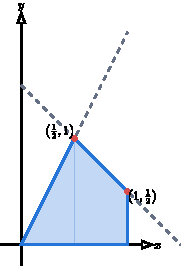
\includegraphics[keepaspectratio,alt={The shaded portion of the support lies below x+y=3/2, split at x=1/2.}]{assets/fig-prob-03-joint-conditional-distribution-diagram-01.pdf}}
  \caption{联合分布 support 中满足 \(X + Y \leq \frac{3}{2}\) 的积分区域}\label{fig-prob-03-joint-conditional-distribution-diagram-01}
  \end{figure}

  在这个图上对联合函数积分即可.
\end{itemize}

\end{qlsolution}

\section{independence of two random variables}\label{independence-of-two-random-variables}

\subsection{independence of two random variables 的三种等价定义}\label{independence-of-two-random-variables-ux7684ux4e09ux79cdux7b49ux4ef7ux5b9aux4e49}

% qlnotes: kind=definition; id=def-03-joint-conditional-distribution-independence-of-random-variables-def-1-joint-distribution-is-pro; concepts=independence-of-random-variables-def-1-joint-distribution-is-pro; aliases=independence of random variables, def 1: joint distribution is product of marginal distributions
\begin{definition}{independence of random variables, def 1: joint distribution is product
of marginal distributions}\label{def-03-joint-conditional-distribution-independence-of-random-variables-def-1-joint-distribution-is-pro}

两个 random variables \(X,Y:\Omega\rightarrow{\mathbb{R}}\) 被称为 independent 的, 如果对于任意的 Borel sets \(A,B \subseteq {\mathbb{R}}\), 都有

\[{\mathbb{P}}(X \in A,Y \in B) = {\mathbb{P}}(X \in A) \cdot {\mathbb{P}}(Y \in B)\]

注意这个定义等价于 for all points \((x,y) \in {\mathbb{R}}^{2}\),

\[F_{X,Y}(x,y) = F_{X}(x)F_{Y}(y)\]

即\textbf{它们的 joint distribution 是它们 marginal distributions 的 product.}

\end{definition}

对于 discrete 和 continuous random variables 而言, 这还意味着 independence 等价于:

\begin{itemize}
\item
  joint pmf 是 marginal pmfs 的 product, for discrete case.
\item
  joint pdf 是 marginal pdfs 的 product, for continuous case.
\end{itemize}

详细而言:

% qlnotes: kind=theorem; id=thm-03-joint-conditional-distribution-discrete-and-continuous-independence-joint-density-is-product-of; concepts=discrete-and-continuous-independence-joint-density-is-product-of; aliases=discrete and continuous independence: joint density is product of marginal densities
\begin{theorem}{discrete and continuous independence: joint density is product of
marginal densities}\label{thm-03-joint-conditional-distribution-discrete-and-continuous-independence-joint-density-is-product-of}

令 \(X,Y\) 是两个 random variables.

\begin{itemize}
\item
  如果 \(X,Y\) 是 discrete random variables, 则它们 independent 的条件等价于对于任意 \(x,y\), 都有

  \[p_{X,Y}(x,y) = p_{X}(x) \cdot p_{Y}(y)\]
\item
  如果 \(X,Y\) 是 continuous random variables, 则它们 independent 的条件等价于对于任意 \(x,y\), 都有

  \[f_{X,Y}(x,y) = f_{X}(x) \cdot f_{Y}(y)\]
\end{itemize}

\end{theorem}

\begin{proof}

discrete case: 显然可得.

continuous case:

\begin{itemize}
\item
  \(F_{X,Y}(x,y) = F_{X}(x)F_{Y}(y)\Longrightarrow f_{X,Y}(x,y) = f_{X}(x) \cdot f_{Y}(y)\): 取偏导数即可.
\item
  \(f_{X,Y}(x,y) = f_{X}(x) \cdot f_{Y}(y)\Longrightarrow F_{X,Y}(x,y) = F_{X}(x)F_{Y}(y)\): 积分即可.
\end{itemize}

\end{proof}

因而对于 independent 的两个 random variables, 固定 \(X = x_{0}\), 那么联合密度函数 \(f_{X,Y}(x_{0},y)\) 就是 \(Y\) 的边际密度函数 \(f_{Y}(y)\) 乘上 一个常数 \(f_{X}(x_{0})\).\\

\begin{qlremark}{Remark}

Recall 两个事件 independence 的定义:

\[{\mathbb{P}}(A \cap B) = {\mathbb{P}}(A) \cdot {\mathbb{P}}(B)\]

也等价于对于任意的 Borel sets \(A,B\) where \({\mathbb{P}}(B) > 0\), 都有

\[{\mathbb{P}}(A \mid B) = {\mathbb{P}}(A)\]

即: 一个事件发生与否都不会对另一个事件发生的概率产生任何影响.

而再看到两个 random variables independence 的定义是:

\[{\mathbb{P}}(X \in A,Y \in B) = {\mathbb{P}}(X \in A) \cdot {\mathbb{P}}(Y \in B)\]

这个定义也当然等价于:

% qlnotes: kind=proposition; id=prop-03-joint-conditional-distribution-independence-of-random-variables-def-2-conditional-distribution; concepts=independence-of-random-variables-def-2-conditional-distribution; aliases=independence of random variables, def 2: conditional distribution is marginal distribution
\begin{proposition}{independence of random variables, def 2: conditional distribution is
marginal distribution}\label{prop-03-joint-conditional-distribution-independence-of-random-variables-def-2-conditional-distribution}

两个 random variables \(X,Y\) 是 independent 的, iff: 对于任意的 Borel sets \(A,B\), 如果\({\mathbb{P}}(Y \in B) > 0\), 则

\[{\mathbb{P}}(X \in A \mid Y \in B) = {\mathbb{P}}(X \in A)\]

即: \textbf{\(X\) 的 conditional distribution, 不论给定 \(Y\) 的任何信息, 都等于 \(X\) 的 marginal distribution.}

\end{proposition}

所以它实际上意义是: \textbf{知道一个 random variable 的任何信息, 对于另外一个都没有任何帮助.}

因而\textbf{它们的 joint distribution 可以分解成 marginal distributions 的 product}.\\

\end{qlremark}

\begin{qlremark}{Remark}

Furthermore: 我们不难发现一件事情, 可以\textbf{在 independence of two events 和 independence of two random variables 之间建立一个桥梁:}

% qlnotes: kind=proposition; id=prop-03-joint-conditional-distribution-independence-of-random-variables-def-3-generated-sigma-algebras; concepts=independence-of-random-variables-def-3-generated-sigma-algebras; aliases=independence of random variables, def 3: generated sigma-algebras
\begin{proposition}{independence of random variables, def 3: generated sigma-algebras}\label{prop-03-joint-conditional-distribution-independence-of-random-variables-def-3-generated-sigma-algebras}

令 \(X,Y\) 是两个 random variables. 则 \(X,Y\) 是 independent 的 iff: \(X\) 生成的 sigma-algebra \(\sigma(X)\) 和 \(Y\) 生成的 sigma-algebra \(\sigma(Y)\) 中分别任取一个事件, 这两个事件都是 independent 的. 即:

\[\forall A \in \sigma(X),\forall B \in \sigma(Y),\quad{\mathbb{P}}(A \cap B) = {\mathbb{P}}(A) \cdot {\mathbb{P}}(B)\]

\end{proposition}

这严格说明了: \textbf{两个 random variables 之间的 independence, 本质上是它们各自蕴含的 information (由 generated sigma-algebra 严格刻画) 的完全不相关}: 对 \(X\) 的观测对于 预测 \(Y\) 的任何行为都不提供任何帮助, 反之亦然.\\

\end{qlremark}

以上就是 independence of two random variables 的定义, 以及其 information geometric intuition.

下面我们讲 independence between two random variables, generalize 到 mutual independence among 任意的 family of random variables.

\subsection{mutual independence of a family of random variables: 强于 pairwise independence}\label{mutual-independence-of-a-family-of-random-variables-ux5f3aux4e8e-pairwise-independence}

我们定义了两个 random variables 的 independence, 但是这个定义可以推广到多个 (甚至 uncountably many) random variables 上.

% qlnotes: kind=definition; id=def-03-joint-conditional-distribution-mutual-independence-of-multiple-random-variables; concepts=mutual-independence-of-multiple-random-variables; aliases=mutual independence of multiple random variables
\begin{definition}{mutual independence of multiple random variables}\label{def-03-joint-conditional-distribution-mutual-independence-of-multiple-random-variables}

令 \(\left\{ {X_{i}:i \in I} \right\}\) 是一个 random variables 的 family, 其中 \(I\) 是一个 index set. 则如果对于任意的 finite subset \(J \subseteq I\), 以及对于任意的 Borel sets \(\left\{ {A_{j}:j \in J} \right\}\), 都有

\[{\mathbb{P}}(X_{j} \in A_{j},\forall j \in J) = \prod\limits_{j \in J}{\mathbb{P}}(X_{j} \in A_{j})\]

则称这个 family of random variables 是 independent 的.

\end{definition}

注意: \textbf{joint mass{ } density 的 factorization 也可以推广到多个 random variables 上.} 有一件事情值得说明: 这里定义的是\textbf{mutual independence}, 也就是说, 对于任意的 finite subset \(J\), 它们的 joint distribution 都 factorizes into product of marginal distributions.

而\textbf{两两 independent 的 random variables family 不一定是 mutual independent 的.} 即: 如果对于任意的 \(i \neq j\), \(X_{i}\) 和 \(X_{j}\) 是 independent 的, 并不意味着对于任意的 finite subset \(J\), \(\left\{ {X_{j}:j \in J} \right\}\) 是 independent 的.

举个例子:

% qlnotes: kind=example; id=ex-03-joint-conditional-distribution-pairwise-independence-does-not-imply-mutual-independence; concepts=pairwise-independence-does-not-imply-mutual-independence; aliases=pairwise independence does NOT imply mutual independence
\begin{example}[pairwise independence does NOT imply mutual independence]\label{ex-03-joint-conditional-distribution-pairwise-independence-does-not-imply-mutual-independence}

假设我们抛掷两枚公平的硬币. 令 \(X,Y\) 是两个 independent 的 random variables, 且都服从 uniform distribution on \(\left\{ {- 1,1} \right\}\). 即:

\[{\mathbb{P}}(X = 1) = {\mathbb{P}}(X = - 1) = \frac{1}{2},\quad{\mathbb{P}}(Y = 1) = {\mathbb{P}}(Y = - 1) = \frac{1}{2}\]

现在, 我们定义第三个 random variable \(Z\) 为前两者的 product:

\[Z = X \cdot Y\]

容易验证: \(X,Y,Z\) 两两 independent, 但不 mutual independent. 因为如果只是知道 \(X\) 的值, 那么我们对于 \(Z\) 的值完全没有信息 (因为有一个完全随机的 \(Y\) 没有任何已知信息); 同样, 如果只是知道 \(Y\) 的值, 那么我们对于 \(Z\) 的值也完全没有信息;

但是, 如果我们同时知道 \(X\) 和 \(Y\) 的值, 那么 \(Z\) 的值就完全确定了.

这说明 \textbf{pairwise independence 只能保证局部的信息解耦, 而 mutual independence 则保证了在这个 family of random variables 之间的全局信息解耦.}

\end{example}

\subsection{\texorpdfstring{independent \(\Longrightarrow\) uncorrelated}{independent \textbackslash Longrightarrow uncorrelated}}\label{independent-longrightarrow-uncorrelated}

Independence 的概念会让我们回忆起另外一个刻画两个 random variables 之间关系的概念: covariance, 它丈量了\textbf{两个 random variables 之间的线性关系}.

covariance 的定义:

\[\text{Cov}(X,Y) := {\mathbb{E}}\lbrack(X - {\mathbb{E}}\lbrack X\rbrack)(Y - {\mathbb{E}}\lbrack Y\rbrack)\rbrack = {\mathbb{E}}\lbrack XY\rbrack - {\mathbb{E}}\lbrack X\rbrack{\mathbb{E}}\lbrack Y\rbrack\]

我们容易发现: \textbf{independence 是一个比 covariance 为 0 (即 uncorrelated) 更强的概念:}

% qlnotes: kind=proposition; id=prop-03-joint-conditional-distribution-independent-uncorrelated; concepts=independent-uncorrelated; aliases=independent 严格强于 uncorrelated
\begin{proposition}{independent 严格强于 uncorrelated}\label{prop-03-joint-conditional-distribution-independent-uncorrelated}

令 \(X,Y\) 是两个 random variables. 则 \(X,Y\) 是 independent 的 \(\Longrightarrow\) \(\text{Cov}(X,Y) = 0\). 但是 \(\text{Cov}(X,Y) = 0\) 不一定 \(\Longrightarrow\) \(X,Y\) 是 independent 的.

\end{proposition}

\begin{proof}

\begin{itemize}
\item
  independence \(\Longrightarrow\) covariance 是 0, 因为 independence 显然 imply\(E\lbrack XY\rbrack = E\lbrack X\rbrack E\lbrack Y\rbrack\), 从而 covariance 的定义式中 \(E\lbrack XY\rbrack - E\lbrack X\rbrack E\lbrack Y\rbrack = 0\).
\item
  有一个经典反例: 考虑 \(X\) 是任意按原点对称的分布, 比如一个 standard normal distribution; 而定义 \(Y = X^{2}\), 此时

  \[\text{Cov}(X,X^{2}) = E\lbrack X \cdot X^{2}\rbrack - E\lbrack X\rbrack E\lbrack X^{2}\rbrack = E\lbrack X^{3}\rbrack - E\lbrack X\rbrack E\lbrack X^{2}\rbrack\]

  由于 \(X\) 的分布是关于原点对称的, \(E\lbrack X^{3}\rbrack = 0\) 且 \(E\lbrack X\rbrack = 0\), 因而 covariance 是 0. 但是 \(X\) 和 \(Y\) 显然不是 independent 的.
\end{itemize}

\end{proof}

\begin{qlremark}{Remark}

本质上, independence 是一种最强的全局信息不相关性. 而 covariance 只度量 linear relationship. 试想: 如果这两个随机变量之间的关系是这样的呢?

\begin{figure}
\centering
\pandocbounded{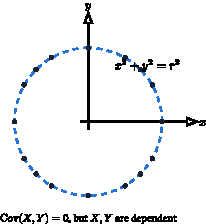
\includegraphics[keepaspectratio,alt={Points constrained to a circle have zero covariance but remain dependent.}]{assets/fig-prob-03-joint-conditional-distribution-diagram-02.pdf}}
\caption{圆周关系说明零协方差不蕴含独立性}\label{fig-prob-03-joint-conditional-distribution-diagram-02}
\end{figure}

那么它们的 covariance 是 0, 但是它们显然不是 independent 的. 所以 covariance 忽略了很多非线性的关系, 而 independence 则完全捕捉了所有的关系.\\

\end{qlremark}

刚才说到, 两个 random variables 的 independence 显然 imply \({\mathbb{E}}\lbrack XY\rbrack = {\mathbb{E}}\lbrack X\rbrack{\mathbb{E}}\lbrack Y\rbrack\). 而 BTW: 这个性质其实\textbf{可以 generalize 到任意 finite number of independent random variables 的 product 上, 并且 我们可以在这些 random variables 上任意地施加 Borel measurable functions}, 只要保证这些函数的 expectation 是 finite 的,

% qlnotes: kind=theorem; id=thm-03-joint-conditional-distribution-independence-implies-expectation-is-closed-under-product; concepts=independence-implies-expectation-is-closed-under-product; aliases=independence \implies expectation is closed under product
\begin{theorem}{independence implies expectation is closed under product}\label{thm-03-joint-conditional-distribution-independence-implies-expectation-is-closed-under-product}

令 \(\left\{ {X_{i}:i \in I} \right\}\) 是一个 independent 的 random variables 的 family, 则对于任意的 finite subset \(J \subseteq I\), 以及对于任意的 Borel measurable functions \(\left\{ {g_{j}:j \in J} \right\}\), 如果 \(\left. {\mathbb{E}}\lbrack \middle| g_{j}(X_{j}) \middle| \rbrack < \infty \right.\) for all \(j \in J\), 则

\[{\mathbb{E}}\left\lbrack {\prod\limits_{j \in J}g_{j}(X_{j})} \right\rbrack = \prod\limits_{j \in J}{\mathbb{E}}\lbrack g_{j}(X_{j})\rbrack\]

特别地, 取每个 \(g_{j}(x) = x\), 则

\[{\mathbb{E}}\left\lbrack {\prod\limits_{j \in J}X_{j}} \right\rbrack = \prod\limits_{j \in J}{\mathbb{E}}\lbrack X_{j}\rbrack\]

\end{theorem}

\begin{proof}

令 \(J = \left\{ {1,2,\ldots,n} \right\}\). 由于 \(X_{1},\ldots,X_{n}\) 是 independent 的, 它们的 joint distribution \(\mu_{\mathbf{X}}\) 是其 marginal distributions \(\mu_{X_{j}}\) 的 product measure:

\[\mu_{\mathbf{X}} = \mu_{X_{1}} \times \mu_{X_{2}} \times \ldots \times \mu_{X_{n}}\]

根据 Change of Variables Formula,

\[{\mathbb{E}}\left\lbrack {\prod\limits_{j = 1}^{n}g_{j}(X_{j})} \right\rbrack = \int_{{\mathbb{R}}^{n}}\left( {\prod\limits_{j = 1}^{n}g_{j}(x_{j})} \right)\, d\mu_{\mathbf{X}}(x_{1},\ldots,x_{n}) = \int_{\mathbb{R}}\ldots\int_{\mathbb{R}}\left( {\prod\limits_{j = 1}^{n}g_{j}(x_{j})} \right)\, d\mu_{X_{1}}(x_{1})\ldots d\mu_{X_{n}}(x_{n})\]

由于被积函数 \(\prod g_{j}(x_{j})\) 是变量分离的, 根据 Fubini's Theorem 可以把积分分解成多个积分的 product:

\[= \left( {\int_{\mathbb{R}}g_{1}(x_{1})\, d\mu_{X_{1}}(x_{1})} \right) \times \ldots \times \left( {\int_{\mathbb{R}}g_{n}(x_{n})\, d\mu_{X_{n}}(x_{n})} \right)\]

其中每一项都是\({\mathbb{E}}\lbrack g_{j}(X_{j})\rbrack\).

\end{proof}

\begin{qlremark}{Remark}

recall: expectation is a linear operator (因而 linearity 是 regardless of independence). 但是它不一定是一个 multiplicative operator.

而这里我们说, \textbf{如果 random variables 是 independent 的, 那么 expectation 就是一个 multiplicative operator.}

\end{qlremark}

实际上: 当这些 Borel measurable functions \(\left\{ {g_{j}:j \in J} \right\}\) 全都 bounded 时, 这个定理其实反向也是成立的:

% qlnotes: kind=theorem; id=thm-03-joint-conditional-distribution-theorem-004; concepts=theorem-004
\begin{theorem}\label{thm-03-joint-conditional-distribution-theorem-004}

令 \(\left\{ {X_{i}:i \in I} \right\}\) 是一个family of random variables. 如果对于任意的 finite subset \(J \subseteq I\), 以及任意的 bounded Borel measurable functions \(\left\{ {g_{j}:j \in J} \right\}\), 都有

\[{\mathbb{E}}\left\lbrack {\prod\limits_{j \in J}g_{j}(X_{j})} \right\rbrack = \prod\limits_{j \in J}{\mathbb{E}}\lbrack g_{j}(X_{j})\rbrack\]

则这个 family of random variables 是 independent 的.

\end{theorem}

\begin{proof}

不妨特取 indicator functions. 对于任意的 Borel sets \(A,B \subseteq {\mathbb{R}}\), 令 \(f(x) = I_{A}(x)\), \(g(y) = I_{B}(y)\). 代入等式得到:

\[{\mathbb{E}}\lbrack I_{A}(X) \cdot I_{B}(Y)\rbrack = {\mathbb{E}}\lbrack I_{A}(X)\rbrack \cdot {\mathbb{E}}\lbrack I_{B}(Y)\rbrack\]

注意到 \(I_{A}(X) \cdot I_{B}(Y) = I_{\{{X \in A,Y \in B}\}}\). 根 据 expectation of indicator function 等于 probability, 我们立刻得到:

\[{\mathbb{P}}(X \in A,Y \in B) = {\mathbb{P}}(X \in A) \cdot {\mathbb{P}}(Y \in B)\]

\end{proof}

注意: \textbf{\(g(x) = x\) 并不是 bounded 的 function, 因而 uncorrelation \(\operatorname{\Longrightarrow\not{}}\) independence.}\\
OK. 以上是 pretty much general properties of independence. 最后我们看一下, 对于 discrete 和 continuous random variables 而言, independence 的 characterization 具体长什么样子.

\subsection{discrete RV independence 的 characterization}\label{discrete-rv-independence-ux7684-characterization}

\begin{qlremark}{Remark}

关于两个 discrete random variables \(X,Y\) 是否 independent 的判断, 还有一个直观的方法.

% qlnotes: kind=proposition; id=prop-03-joint-conditional-distribution-discrete-rv-independence-characterization; concepts=discrete-rv-independence-characterization; aliases=discrete RV independence 的 characterization
\begin{proposition}{discrete RV independence 的 characterization}\label{prop-03-joint-conditional-distribution-discrete-rv-independence-characterization}

两个 discrete random variables \(X,Y\) 是 independent 的 iff 它们的 joint pmf as a matrix 有 rank 1(每行每列都互为倍数).

\end{proposition}

\begin{proof}

note: 一个矩阵 \(M\) 的 rank 等于 1 iff 它可以被分解为两个向量的 outer product :

\[M = \mathbf{u}\mathbf{v}^{\top}\]

~where \(\mathbf{u}\) 和 \(\mathbf{v}\) 是非零列向量.

(\(\Longrightarrow\)): 如果 independent, 那么对于所有 \(i,j\), joint probability \(p_{ij} = {\mathbb{P}}(X = x_{i},Y = y_{j})\) 满足:

\[p_{ij} = {\mathbb{P}}(X = x_{i}) \cdot {\mathbb{P}}(Y = y_{j})\]

如果我们定义向量 \(\mathbf{p}_{X} = \lbrack p_{X}(x_{1}),p_{X}(x_{2}),\ldots\rbrack^{\top}\) 和 \(\mathbf{p}_{Y} = \lbrack p_{Y}(y_{1}),p_{Y}(y_{2}),\ldots\rbrack^{\top}\), 那么整个联合分布矩阵 \(P\) 就可以写成:

\[P = \mathbf{p}_{X}\mathbf{p}_{Y}^{\top}\]

这正是 Rank 1 矩阵的标准形式.

(\(\Longleftarrow\)) 如果 \(P\) 的 rank 为 1, 那么存在向量 \(\mathbf{u}\) 和 \(\mathbf{v}\) 使得 \(p_{ij} = u_{i}v_{j}\).由于 \(\sum_{i,j}p_{ij} = 1\), 我们可以归一化这两个向量, 使得 \(\sum u_{i} = 1\) 且 \(\sum v_{j} = 1\).此时, \(u_{i}\) 恰好就是 \(X\) 的 marginal PMF, \(v_{j}\) 恰好就是 \(Y\) 的 marginal PMF. 因此满足 \(p_{ij} = p_{i} \cdot p_{j}\), 即两个变量独立.

\end{proof}

% qlnotes: kind=example; id=ex-03-joint-conditional-distribution-example-004; concepts=example-004
\begin{example}\label{ex-03-joint-conditional-distribution-example-004}

\[\begin{matrix}
{P = X \smallsetminus Y} & 0 & {1\ } & {\text{Marginal}\ {\mathbb{P}}(X)} \\
0 & 0.4 & 0.1 & 0.5 \\
1 & 0.4 & 0.1 & 0.5 \\
{\text{Marginal}\ {\mathbb{P}}(Y)} & 0.8 & 0.2 & 1.0
\end{matrix}\]

这里的 \(X,Y\) 就是 independent 的 random variables.

\end{example}

\end{qlremark}

\subsection{continuous RV independence 的 geometric intuition}\label{continuous-rv-independence-ux7684-geometric-intuition}

对于 independent continuous random variables \(X,Y\), 它的 characterization 我们已经知道了: 即 joint pdf factorizes into marginal pdfs. 这一个 characterization 的 geometric intuition 是:

\begin{itemize}
\item
  joint pdf 的 support set 一定是一个矩形 (不一定 bounded)
\item
  joint pdf 的\textbf{每个维度上的任意截面的形状都是一样的} (因为固定 \(x\), 则 \(y\) 方向的性质只由 \(f_{Y}\) 决定.)

  即: 固定 \(x\), \(y\)-distribution 的横截面永远长得像 \(f_{Y}\), 只是乘上了一个常数 \(f_{X}(x)\) 而已. 同样的, 固定 \(y\), \(x\) 分布的横截面永远长得像 \(f_{X}\), 只是乘上了一个常数 \(f_{Y}(y)\) 而已.
\end{itemize}

\begin{figure}
\centering
\pandocbounded{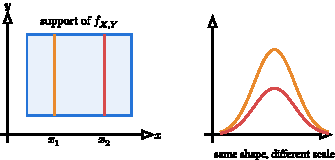
\includegraphics[keepaspectratio,alt={A rectangular joint support whose vertical cross-sections share one shape at different scales.}]{assets/fig-prob-03-joint-conditional-distribution-diagram-03.pdf}}
\caption{独立连续随机变量的矩形 support 与等形横截面}\label{fig-prob-03-joint-conditional-distribution-diagram-03}
\end{figure}

\section{conditional distribution function and density}\label{conditional-distribution-function-and-density}

\subsection{conditional distribution and its distribution function}\label{conditional-distribution-and-its-distribution-function}

% qlnotes: kind=definition; id=def-03-joint-conditional-distribution-conditional-distribution; concepts=conditional-distribution; aliases=conditional distribution
\begin{definition}{conditional distribution}\label{def-03-joint-conditional-distribution-conditional-distribution}

给定 random variables \(X,Y:\Omega\rightarrow{\mathbb{R}}\), 我们定义 the conditional distribution of \(X\) given \(Y = y\) 为 the probability measure \({\mathbb{P}}^{X|Y = y}\):

\[{\mathbb{P}}^{X|Y = y}(A) := \lim\limits_{h\rightarrow 0^{+}}{\mathbb{P}}(X \in A \mid y \leq Y \leq y + h),\quad\forall A \in \mathcal{B}({\mathbb{R}})\]

并将 function \(F_{X|Y = y}:{\mathbb{R}}\rightarrow{\mathbb{R}}\) defined by \(F_{X|Y = y}(x) := {\mathbb{P}}^{X|Y = y}(( - \infty,x\rbrack)\):

\[\left. F_{X|Y}(x \middle| y) := \lim\limits_{h\rightarrow 0^{+}}{\mathbb{P}}(X \leq x \mid y \leq Y \leq y + h) \right.\]

称为 the conditional distribution function of \(X\) given \(Y = y\).

\end{definition}

\begin{qlremark}{Remark}

注意: 每个取值 \(y\) 都对应一个 conditional distribution measure \({\mathbb{P}}^{X|Y = y}\) 和一个 conditional distribution function \(F_{X|Y = y}\). 因此, conditional distribution 和 conditional distribution function 都是一个 family of measures/functions, 而不是一个 measure/function.

也就是说, 一个 random variable 可以 induce 出另一个 random variable 的可能 uncountably many 个 conditional distribution.

\end{qlremark}

\begin{qlremark}{Remark}

如果 \(X,Y\) 是两个 discrete random variables, 那么它们的 conditional distribution 就很简单了.

\[{\mathbb{P}}^{X|Y = y}(\left\{ x \right\}) = \frac{{\mathbb{P}}(X = x,Y = y)}{{\mathbb{P}}(Y = y)}\]

以及

\[F_{X|Y = y}(x) = \sum\limits_{t \leq x}\frac{{\mathbb{P}}(X = t,Y = y)}{{\mathbb{P}}(Y = y)}\]

其他情况稍复杂一些. 但是我们可以确定的是:

\end{qlremark}

\subsection{conditional density for random variables jointly continuous}\label{conditional-density-for-random-variables-jointly-continuous}

% qlnotes: kind=theorem; id=thm-03-joint-conditional-distribution-jointly-continuous-rvs-defined-conditional-density; concepts=jointly-continuous-rvs-defined-conditional-density; aliases=jointly continuous RVs 之间所有 defined 处总有 conditional density
\begin{theorem}{jointly continuous RVs 之间所有 defined 处总有 conditional density}\label{thm-03-joint-conditional-distribution-jointly-continuous-rvs-defined-conditional-density}

令 \(\mathbf{X} = (X,Y)^{T}\) 是一个 continuous random vector, 则对于任意 \(y\) 使得 \(f_{Y}(y) > 0\), 都有 conditional distribution of \(X\) given \(Y = y\) 的 pdf:

\[\left. f_{X|Y}(x \middle| y) := \frac{f_{X,Y}(x,y)}{f_{Y}(y)} \right.\]

即: \(\forall x \in {\mathbb{R}}\) 有:

\[\left. F_{X|Y}(x \middle| y) = \int_{- \infty}^{x}\frac{f_{X,Y}(t,y)}{f_{Y}(y)}\, dt \right.\]

\end{theorem}

\begin{proof}

注意: \((X,Y)^{T}\) 是 continuous random vector \(\Longrightarrow\) \(Y\) 是一个 continuous random variable. 因而 因而 \(f_{Y}(y)\) 是 well-defined 的. (反过来不成立) 取 \(y\) s.t. \(f_{Y}(y) > 0\).

则

\[\begin{matrix}
{{\mathbb{P}}^{X \mid Y = y}(A)} & {= \lim\limits_{h\rightarrow 0^{+}}{\mathbb{P}}(X \in A \mid y \leq Y \leq y + h)} \\
 & {= \lim\limits_{h\rightarrow 0^{+}}\frac{{\mathbb{P}}(X \leq x,y \leq Y \leq y + h)}{{\mathbb{P}}(y \leq Y \leq y + h)} = \lim\limits_{h\rightarrow 0^{+}}\frac{F_{X,Y}(x,y + h) - F_{X,Y}(x,y)}{F_{Y}(y + h) - F_{Y}(y)}} \\
 & {= \frac{\partial_{y}F_{X,Y}(x,y)}{f_{Y}(y)} = \int_{- \infty}^{x}\frac{f_{X,Y}(s,y)}{f_{Y}(y)}ds}
\end{matrix}\]

因而, \(\left. f_{X|Y}(x \middle| y) := \frac{f_{X,Y}(x,y)}{f_{Y}(y)} \right.\) 是 \(F_{X|Y = y}\) 的 pdf.

\end{proof}

\begin{qlremark}{Remark}

为了保证 continuous random vector 下分量之间的 conditional distribution 总是 (a.e.) 拥有 pdf 的, 我们可以 给 not well-defined 处下定义: 如果 \(f_{Y}(y) = 0\), 就直接 set \(\left. f_{X|Y}(x \middle| y) = 0 \right.\) for all \(x\).

在这个定义下: continuous random vector 下分量之间的 conditional distribution 也总是 continuous 的.

\end{qlremark}

\subsection{Law of Total Probability for continuous random vector}\label{law-of-total-probability-for-continuous-random-vector}

% qlnotes: kind=theorem; id=thm-03-joint-conditional-distribution-theorem-006; concepts=theorem-006
\begin{theorem}\label{thm-03-joint-conditional-distribution-theorem-006}

令 \(\mathbf{X} = (X,Y)^{T}\) 是一个 continuous random vector, 则对于任意 \(A \in \mathcal{B}({\mathbb{R}})\),

\[{\mathbb{P}}((X,Y) \in A) = \int_{- \infty}^{+ \infty}{\mathbb{P}}((X,y) \in A \mid Y = y)f_{Y}(y)dy\]

\end{theorem}

\begin{proof}

注意:

\[{\mathbb{P}}\left( {Y \in \left\{ {y \in {\mathbb{R}}:f_{Y}(y) = 0} \right\}} \right) = 0\]

即, \(\left\{ {Y \in f_{Y}^{- 1}(\left\{ 0 \right\})} \right\}\) 是一个 null set. (不是说 \(f_{Y}(y) = 0\) 的 \(y\) 是 null set, 意思是说 \(Y\) 落在这些 \(y\) 上的事件是 null set.)

因而 compute:

\[\begin{matrix}
{{\mathbb{P}}(X \in ( - \infty,x\rbrack,Y \leq y)} & {= {\mathbb{P}}\left( {X \in ( - \infty,x\rbrack,\left\{ {Y \leq y} \right\} \cap \left\{ {Y \notin f_{Y}^{- 1}(\left\{ 0 \right\})} \right\}} \right) = \int_{( - \infty,y\rbrack \cap f_{Y}^{- 1}{({\{ 0\}}^{c})}}\int_{- \infty}^{\infty}f_{X,Y}(s,t)dsdt} \\
 & {= \int_{( - \infty,y\rbrack \cap f_{Y}^{- 1}((0, + \infty))}\left( {\int_{- \infty}^{x}\frac{f_{X,Y}(s,t)}{f_{Y}(t)}ds} \right)f_{Y}(t)dt} \\
 & {= \int_{( - \infty,y\rbrack \cap f_{Y}^{- 1}((0, + \infty))}{\mathbb{P}}(X \leq x \mid Y = t)f_{Y}(t)dt} \\
 & {= \int_{( - \infty,y\rbrack \cap f_{Y}^{- 1}((0, + \infty))}{\mathbb{P}}(X \leq x \mid Y = t)f_{Y}(t)dt + \int_{( - \infty,y\rbrack \cap f_{Y}^{- 1}({\{ 0\}})}{\mathbb{P}}(X \leq x \mid Y = t)f_{Y}} \\
 & {= \int_{( - \infty,y\rbrack}{\mathbb{P}}(X \leq x \mid Y = t)f_{Y}(t)dt} \\
 & {= \int_{- \infty}^{y}{\mathbb{P}}(X \leq x \mid Y = t)f_{Y}(t)dt}
\end{matrix}\]

\end{proof}

\begin{qlremark}{Remark}

recall 最普通的全概率公式: 把样本空间 partition 成几个 disjoint 的事件 \(B_{1},\cdots,B_{n}\), 则任意事件\(A\) 等于它在每个 \(B_{i}\) 上的 conditional probability 的和:

\[{\mathbb{P}}(A) = \sum\limits_{i = 1}^{n}{\mathbb{P}}(A \cap B_{i}) = \sum\limits_{i = 1}^{n}{\mathbb{P}}(A \mid B_{i}){\mathbb{P}}(B_{i})\]

这很容易理解. 而这里的 law of total probability for continuous random vector 就是这个公式在 continuous case 的推广:

由于在每一点 \(y\) 上, \((X,Y) \in A\) 的概率都有一个 conditional distribution \(\left. (X,Y) \in A \middle| Y = y \right.\), 因而 \((X,Y) \in A\) 的概率就等于这个 conditional distribution 在所有 \(y\) 上的加权和, 权重就是 \(Y\) 的 pdf \(f_{Y}(y)\). 因而才有

\[{\mathbb{P}}((X,Y) \in A) = \int_{- \infty}^{+ \infty}{\mathbb{P}}((X,y) \in A \mid Y = y)f_{Y}(y)dy\]

\end{qlremark}

% qlnotes: kind=example; id=ex-03-joint-conditional-distribution-example-005; concepts=example-005
\begin{example}\label{ex-03-joint-conditional-distribution-example-005}

考虑 random vector \(\mathbf{X} = (X,Y)^{T}\) with joint pdf

\[f_{X,Y}(x,y) = \left\{ \begin{matrix}
{4xy,} & {\text{if}\ 0 \leq x \leq 1,0 \leq y \leq 1} \\
{0,} & \text{otherwise}
\end{matrix} \right.\]

计算: \(f_{X},f_{Y},f_{X|Y},f_{Y|X}\).

\end{example}

\begin{qlsolution}{Solution}

首先计算 margianl pdfs:

\[f_{X}(x) = \int_{- \infty}^{+ \infty}f_{X,Y}(x,y)dy = \int_{0}^{1}4xydy = 2x,\text{for}\ 0 \leq x \leq 1\]

and

\[f_{Y}(y) = \int_{- \infty}^{+ \infty}f_{X,Y}(x,y)dx = \int_{0}^{1}4xydx = 2y,\text{for}\ 0 \leq y \leq 1\]

由于这是一个 continuous random vector, 因而根据\hyperref[thm-03-joint-conditional-distribution-jointly-continuous-rvs-defined-conditional-density]{Theorem~\ref*{thm-03-joint-conditional-distribution-jointly-continuous-rvs-defined-conditional-density}} 可以得到:

\[f_{X \mid Y}(x \mid y) = \left\{ \begin{matrix}
{\frac{f_{X,Y}(x,y)}{f_{Y}(y)} = \frac{4xy}{2y} = 2x,} & {\text{if}\ x \in \lbrack 0,1\rbrack,} \\
{0,} & \text{otherwise.}
\end{matrix} \right.\]

同理计算出

\[f_{Y \mid X}(y \mid x) = \left\{ \begin{matrix}
{\frac{f_{X,Y}(x,y)}{f_{X}(x)} = \frac{4xy}{2x} = 2y,} & {\text{if}\ y \in \lbrack 0,1\rbrack,} \\
{0,} & \text{otherwise.}
\end{matrix} \right.\]

\end{qlsolution}

\section{conditional expectation}\label{conditional-expectation}

% qlnotes: kind=definition; id=def-03-joint-conditional-distribution-conditional-expectation; concepts=conditional-expectation; aliases=conditional expectation
\begin{definition}{conditional expectation}\label{def-03-joint-conditional-distribution-conditional-expectation}

令 \(X,Y:\Omega\rightarrow{\mathbb{R}}\) 为 RVs. 对于 \(y \in {\mathbb{R}}\) where \(F_{X|Y} = {\mathbb{P}}^{X|Y = y}(X \leq x)\) is defined (这个条件对于 discrete 是筛选掉 \({\mathbb{P}}(y) = 0\) 的点, 对于 continuous 这是为了筛选掉 \(f_{Y} = 0\) 的点), 我们定义 conditional expectation:

\[\left. {\mathbb{E}}\lbrack X \middle| Y = y\rbrack := \int_{- \infty}^{\infty}x\, d{\mathbb{P}}^{X|Y = y}(x) \right.\]

特别地, 如果\((X,Y)\) 是一个 discrete random vector, 则它即是:

\[\left. {\mathbb{E}}\lbrack X \middle| Y = y\rbrack = \sum\limits_{x}x{\mathbb{P}}(X \middle| Y)(x \middle| y) = \sum\limits_{x}x{\mathbb{P}}(X = x \middle| Y = y) \right.\]

而如果 \((X,Y)\) 是一个 (absolutely) continuous random vector, 则它即是:

\[\left. {\mathbb{E}}\lbrack X \middle| Y = y\rbrack = \int_{- \infty}^{\infty}xf_{X|Y}(x \middle| y)\, dx \right.\]

\end{definition}

\begin{qlremark}{Remark}

注意: conditional expectation 对于给定的 \(y\) 是一个值; 而它也整体是一个 function of \(y\), 同时也是 function from the sample space \(\Omega\) (更准确而言是 \(\left\{ {\omega \in \Omega:f_{Y}(Y(\omega)) > 0} \right\}\), 但是去掉的 这个集合的测度为零, 所以不用管, a.e. define 即可).

对于 \(\omega \in \Omega\),

\[\left. {\mathbb{E}}\lbrack X \middle| Y\rbrack:\omega\mapsto{\mathbb{E}}\lbrack X \middle| Y = Y(\omega)\rbrack \right.\]

Notice: 这个函数是一个 random variable. 同理, 我们可以构造 conditional expectation given multiple random variables \(\left. {\mathbb{E}}\lbrack X \middle| Y_{1},\cdots,Y_{n}\rbrack \right.\). 但是暂时不谈论这个.

\end{qlremark}

% qlnotes: kind=proposition; id=prop-03-joint-conditional-distribution-independence-conditional-distribution-density-expectation; concepts=independence-conditional-distribution-density-expectation; aliases=independence 让 conditional distribution, density 和 expectation 都退化
\begin{proposition}{independence 让 conditional distribution, density 和 expectation 都退化}\label{prop-03-joint-conditional-distribution-independence-conditional-distribution-density-expectation}

如果 \(X,Y\) 是 independent 的, 那么在任意 defined \(y\) 上,

\[F_{X|Y = y} = F_{X},\quad f_{X|Y = y} = f_{X},\]

以及

\[\left. \quad{\mathbb{E}}\lbrack X \middle| Y\rbrack = {\mathbb{E}}\lbrack X\rbrack \right.\]

\end{proposition}

% qlnotes: kind=example; id=ex-03-joint-conditional-distribution-example-006; concepts=example-006
\begin{example}\label{ex-03-joint-conditional-distribution-example-006}

\textbf{(constant random variable 的 conditional expectation)}

令 \(X := b\) 为一个 constant random variable. \(Y\) 为一个 (absolutely) continuous random variable. compute: \(\left. {\mathbb{E}}\lbrack X \middle| Y\rbrack \right.\) when \(f_{Y}(y) > 0\).

\end{example}

\begin{qlsolution}{Solution}

\[\begin{matrix}
{F_{X,Y}(x,y) = {\mathbb{P}}(X \leq x,Y \leq y) = \{ F_{Y}(y),} & {\text{if}\ x \leq b,} \\
{0,} & {\text{if}\ x > b = F_{X}(x) \cdot F_{Y}(y)}
\end{matrix}\]

因而它们 independent (当然,,) 因而

\[\left. {\mathbb{E}}\lbrack X \middle| Y\rbrack = {\mathbb{E}}\lbrack X\rbrack = b \right.\]

\end{qlsolution}

为什么我们要提及这个很呆的例子 因为我们要说一个很呆但是要说一下的事情:

% qlnotes: kind=proposition; id=prop-03-joint-conditional-distribution-proposition-010; concepts=proposition-010
\begin{proposition}\label{prop-03-joint-conditional-distribution-proposition-010}

conditional expectation 满足 linear property. 即任取 \(a,b \in {\mathbb{R}}\),

\[\left. {\mathbb{E}}\lbrack aX + b \middle| Y\rbrack = a{\mathbb{E}}\lbrack X \middle| Y\rbrack + b \right.\]

\end{proposition}

% qlnotes: kind=example; id=ex-03-joint-conditional-distribution-example-007; concepts=example-007
\begin{example}\label{ex-03-joint-conditional-distribution-example-007}

(computation exercise) 令 \(X,Y\) 为 RVs with joint pdf

\[f_{X,Y}(x,y) = \left\{ \begin{matrix}
{\frac{1}{y}e^{- \frac{x}{y}}e^{- y},} & {x > 0,y > 0} \\
{0,} & \text{otherwise}
\end{matrix} \right.\]

计算: \(\left. {\mathbb{E}}\lbrack X \middle| Y = y\rbrack \right.\).

\end{example}

\begin{qlsolution}{Solution}

根据 \hyperref[thm-03-joint-conditional-distribution-jointly-continuous-rvs-defined-conditional-density]{Theorem~\ref*{thm-03-joint-conditional-distribution-jointly-continuous-rvs-defined-conditional-density}} 和 \hyperref[def-03-joint-conditional-distribution-conditional-expectation]{Definition~\ref*{def-03-joint-conditional-distribution-conditional-expectation}}, 我们就是要做两件事情: 一个是计算 \(f_{Y}\), 然后 根据 \(f_{Y}\) 和 \(f_{X,Y}\) 计算出 \(f_{X|Y}\), 最后根据 \(f_{X|Y}\) 积分计算出 \(\left. {\mathbb{E}}\lbrack X \middle| Y\rbrack \right.\).

那么

\[f_{Y}(y) = \int_{- \infty}^{+ \infty}f_{X,Y}(x,y)dx = e^{- y}\int_{0}^{+ \infty}\frac{1}{y}e^{- x/y}dx = e^{- y},y > 0\]

我们发现 \(Y \sim \text{Exp}(1)\). 然后对于 \(y > 0\),

\[f_{X \mid Y}(x \mid y) = \frac{f_{X,Y}(x,y)}{f_{Y}(y)} = \frac{1}{y}e^{- x/y}\]

因而 \(\left. X \middle| Y = y \sim \text{Exp}(1/y) \right.\). 最后,

\[{\mathbb{E}}\lbrack X \mid Y = y\rbrack = \int_{- \infty}^{+ \infty}xf_{X \mid Y}(x \mid y)dx = \frac{1}{y}\int_{0}^{+ \infty}xe^{- x/y}dx = y\]

而对于 \(y \leq 0\), 因为 \(f_{Y}(y) = 0\), \({\mathbb{E}}\lbrack X \mid Y = y\rbrack\) is not defined.

\end{qlsolution}

//TODO: 如果 \(X\) 是 continous 的, 而 \(Y\) 是 discrete 的, 那么我们怎么 define conditional distribution, 以及 expectation 呢? 这个时候我们就需要用到 之前说的 generated \(\sigma\)-algebra 的概念了.

\section{law of total expectation}\label{law-of-total-expectation}

% qlnotes: kind=theorem; id=thm-03-joint-conditional-distribution-law-of-total-expectation; concepts=law-of-total-expectation; aliases=law of total expectation
\begin{theorem}{law of total expectation}\label{thm-03-joint-conditional-distribution-law-of-total-expectation}

令 \(X,Y:\Omega\rightarrow{\mathbb{R}}\) 为 RVs, 我们知道它们的 conditional expectation \(\left. {\mathbb{E}}\lbrack X \middle| Y\rbrack \right.\) 也是一个 \(\Omega\rightarrow{\mathbb{R}}\) 的 RV.

如果 \(\left. {\mathbb{E}}\lbrack \middle| {\mathbb{E}}\lbrack X \middle| Y\rbrack \middle| \rbrack < \infty \right.\), 则

\[\left. {\mathbb{E}}\lbrack X\rbrack = {\mathbb{E}}\lbrack{\mathbb{E}}\lbrack X \middle| Y\rbrack\rbrack \right.\]

\end{theorem}

\begin{proof}

对于更加严格的 conditional expectation 的定义而言 (as an orthogonal projection from \(L^{2}(\Omega,\mathcal{F},{\mathbb{P}})\) onto the subspace of \(Y\)-measurable functions), 这个定理是 trivial 的, 直接 follow from def. 在该定义中, \(\left. {\mathbb{E}}\lbrack X \middle| Y\rbrack \right.\) 被定义为一个 \(\sigma(Y)\)-measurable function \(Z\), 使得对于任意 \(A \in \sigma(Y)\), 都有

\[\int_{A}Z\, d{\mathbb{P}} = \int_{A}X\, d{\mathbb{P}}\]

那么取 \(A = \Omega\), 自然得到.

而我们目前的定义下, 要证明它则要对于 discrete 和 continuous 两种情况分别计算证明. (recall Lebesgue Decomposition Theorem: 任意 measure 都可以被分解成一个 discrete 的部分和一个 continuous 的部分以及一个 可以忽略的 singular 的部分. 因而证明了 discrete 和 continuous 两种情况即可.)

For discrete case:

\[\begin{matrix}
{{\mathbb{E}}\lbrack{\mathbb{E}}\lbrack X \mid Y\rbrack\rbrack} & {= {\mathbb{E}}_{\omega}\lbrack{\mathbb{E}}\lbrack X \mid Y = Y(\omega)\rbrack\rbrack = {\mathbb{E}}_{\omega}\left\lbrack {\sum\limits_{x}x{\mathbb{P}}(X = x \mid Y = Y(\omega))} \right\rbrack} \\
 & {= \sum\limits_{x}x{\mathbb{E}}_{\omega}\lbrack{\mathbb{P}}(X = x \mid Y = Y(\omega))\rbrack} \\
 & {= \sum\limits_{x}x\sum\limits_{y}{\mathbb{P}}(X = x \mid Y = y) \cdot {\mathbb{P}}(Y = y)} \\
 & {= \sum\limits_{x}x\sum\limits_{y}{\mathbb{P}}(X = x,Y = y)} \\
 & {= \sum\limits_{x}x{\mathbb{P}}(X = x) = {\mathbb{E}}\lbrack X\rbrack}
\end{matrix}\]

For continuous case:

\[\begin{matrix}
{{\mathbb{E}}\lbrack{\mathbb{E}}\lbrack X \mid Y\rbrack\rbrack} & {= {\mathbb{E}}_{\omega}\left\lbrack {\int_{- \infty}^{+ \infty}xf_{X \mid Y}(x \mid Y(\omega))dx} \right\rbrack = \int_{- \infty}^{+ \infty}x{\mathbb{E}}_{\omega}\left\lbrack {f_{X \mid Y}(x \mid Y(\omega))} \right\rbrack dx} \\
 & {= \int_{- \infty}^{+ \infty}x\int_{- \infty}^{+ \infty}f_{X \mid Y}(x \mid y)f_{Y}(y)dydx} \\
 & {= \int_{- \infty}^{+ \infty}\int_{- \infty}^{+ \infty}xf_{X,Y}(x,y)dxdy} \\
 & {= \int_{- \infty}^{+ \infty}x\int_{- \infty}^{+ \infty}f_{X,Y}(x,y)dxdx} \\
 & {= \int_{- \infty}^{+ \infty}xf_{X}(x)dx = {\mathbb{E}}\lbrack X\rbrack}
\end{matrix}\]

\end{proof}

% qlnotes: kind=example; id=ex-03-joint-conditional-distribution-example-008; concepts=example-008
\begin{example}\label{ex-03-joint-conditional-distribution-example-008}

(\textbf{fair coin toss}) 我们投掷一枚 fair coin. \(X_{1}\): 直到 HH 出现钱, 投掷的次数;

\(X_{2}\): 直到 HT 出现钱, 投掷的次数.

问题: 计算 \({\mathbb{E}}\lbrack X_{1}\rbrack\) 和 \({\mathbb{E}}\lbrack X_{2}\rbrack\).

\end{example}

\begin{qlsolution}{Solution}

We condition on 第一次 toss \(Y_{1}\), 以及第二次 toss \(Y_{2}\).

\[\begin{matrix}
{{\mathbb{E}}\left\lbrack X_{1} \right\rbrack} & {= {\mathbb{E}}\left\lbrack {{\mathbb{E}}\left\lbrack {X_{1} \mid Y_{1}} \right\rbrack} \right\rbrack = \frac{1}{2}{\mathbb{E}}\left\lbrack {X_{1} \mid Y_{1} = H} \right\rbrack + \frac{1}{2}{\mathbb{E}}\left\lbrack {X_{1} \mid Y_{1} = T} \right\rbrack} \\
 & {= \frac{1}{2}\left( {\frac{1}{2}{\mathbb{E}}\left\lbrack {X \mid Y_{1} = H,Y_{2} = H} \right\rbrack + \frac{1}{2}{\mathbb{E}}\left\lbrack {X \mid Y_{1} = H,Y_{2} = T} \right\rbrack} \right) + \frac{1}{2}\left( {1 + {\mathbb{E}}\left\lbrack X_{1} \right\rbrack} \right)} \\
 & {= \frac{1}{2}\left( {\frac{2}{2} + \frac{1}{2}\left( {{\mathbb{E}}\left\lbrack X_{1} \right\rbrack + 2} \right)} \right) + \frac{1}{2}\left( {1 + {\mathbb{E}}\left\lbrack X_{1} \right\rbrack} \right).}
\end{matrix}\]

解出 \({\mathbb{E}}\lbrack X_{1}\rbrack = 6\). 同理, 可以解出 \({\mathbb{E}}\lbrack X_{2}\rbrack = 4\).

\end{qlsolution}

% qlnotes: kind=example; id=ex-03-joint-conditional-distribution-example-009; concepts=example-009
\begin{example}\label{ex-03-joint-conditional-distribution-example-009}

一只鸡在一段时间内下 \(N\) 个蛋, 其中 \(N \sim \text{Pois}(\lambda)\). 每只蛋孵化成小鸡的概率为 \(p\), 互相独立. 令 \(K\) 表示孵化成小鸡的蛋的数量, 计算 \(\left. K \middle| N,{\mathbb{E}}\lbrack K\rbrack \right.\), 以及 \(K\) 的 distribution.

\end{example}

\begin{qlsolution}{Solution}

由题意得

\[\left. {\mathbb{P}}(K = k \middle| N = n) = \left( \frac{n}{k} \right)p^{k}(1 - p)^{n - k} \right.\]

因此, \(\left. K \middle| N = n \sim \text{Bin}(n,p) \right.\) 因而 \(\left. {\mathbb{E}}\lbrack K \middle| N = n\rbrack = np \right.\). 由 law of total expectation,

\[\left. {\mathbb{E}}\lbrack K\rbrack = {\mathbb{E}}\lbrack{\mathbb{E}}\lbrack K \middle| N\rbrack\rbrack = {\mathbb{E}}\lbrack N\rbrack \cdot p = \lambda \right.\]

然后由 law of total probability,

\[\begin{matrix}
{{\mathbb{P}}(K = k)} & \left. = \sum\limits_{n = k}^{+ \infty}{\mathbb{P}}(K = k,N = n) = \sum\limits_{n = k}^{+ \infty}{\mathbb{P}}(K = k \middle| N = n) \cdot {\mathbb{P}}(N = n) \right. \\
 & {= \sum\limits_{n = k}^{+ \infty}\left( \frac{n}{k} \right)p^{k}(1 - p)^{n - k} \cdot \frac{\lambda^{n}e^{- \lambda}}{n!}} \\
 & {= \sum\limits_{n = k}^{+ \infty}\frac{n!}{k!(n - k)!}p^{k}(1 - p)^{n - k} \cdot \frac{\lambda^{n}e^{- \lambda}}{n!}} \\
 & {= \sum\limits_{n = k}^{+ \infty}\frac{\lambda^{n}e^{- \lambda}}{k!(n - k)!}p^{k}(1 - p)^{n - k}} \\
 & {= \sum\limits_{n = k}^{+ \infty}\frac{(\lambda p)^{k}(\lambda(1 - p))^{n - k}e^{- \lambda}}{k!(n - k)!}} \\
 & {= \frac{(\lambda p)^{k}e^{- \lambda}}{k!}\sum\limits_{n = k}^{+ \infty}\frac{(\lambda(1 - p))^{n - k}}{(n - k)!}} \\
 & {= \frac{(\lambda p)^{k}e^{- \lambda}}{k!}\sum\limits_{m = 0}^{+ \infty}\frac{(\lambda(1 - p))^{m}}{m!}} \\
 & {= \frac{(\lambda p)^{k}e^{- \lambda}}{k!} \cdot e^{\lambda(1 - p)} = \frac{(\lambda p)^{k}e^{- \lambda p}}{k!}}
\end{matrix}\]

因而 \(K \sim \text{Pois}(\lambda p)\).

\end{qlsolution}

% qlnotes: kind=example; id=ex-03-joint-conditional-distribution-example-010; concepts=example-010
\begin{example}\label{ex-03-joint-conditional-distribution-example-010}

令 \((X,Y)\) 为一对 continuous RVs with joint pdf:

\[f_{X,Y}(x,y) = 2e^{- (x + 2y)}\mathbf{1}_{\{{x > 0,y > 0}\}}\]

首先, verify \(f_{X,Y}\) is a valid joint pdf, 然后计算 \(\left. {\mathbb{E}}\lbrack X \middle| Y = y\rbrack \right.\) 和 \({\mathbb{E}}\lbrack X\rbrack\).

\end{example}

\begin{qlsolution}{Solution}

\[\int_{0}^{\infty}\int_{0}^{\infty}2e^{- (x + 2y)}dxdy = \int_{0}^{\infty}2e^{- 2y}\left( {\int_{0}^{\infty}e^{- x}dx} \right)dy = \int_{0}^{\infty}2e^{- 2y}dy = 1\]

verify 很简单. 然后我们首先计算 density of \(Y\):

\[f_{Y}(y) = \int_{0}^{\infty}2e^{- (x + 2y)}dx = 2e^{- 2y},\quad y > 0\]

然后计算 conditional density of \(X\) given \(Y = y\):

\[f_{X \mid Y}(x \mid y) = \frac{f_{X,Y}(x,y)}{f_{Y}(y)} = e^{- x},\quad x > 0\]

因而 by \hyperref[def-03-joint-conditional-distribution-conditional-expectation]{Definition~\ref*{def-03-joint-conditional-distribution-conditional-expectation}},

\[{\mathbb{E}}\lbrack X \mid Y = y\rbrack = \int_{0}^{\infty}xe^{- x}dx = 1\]

然后 by law of total expectation,

\[\left. {\mathbb{E}}\lbrack X\rbrack = {\mathbb{E}}\lbrack{\mathbb{E}}\lbrack X \middle| Y\rbrack\rbrack = {\mathbb{E}}\lbrack 1\rbrack = 1 \right.\]

since \(\left. {\mathbb{E}}\lbrack X \middle| Y\rbrack \right.\) is a constant function.

\end{qlsolution}

\chapter{Behaviors of a sequence of random variables}\label{behaviors-of-a-sequence-of-random-variables}

\section{Toolbox review: inequalities in probability}\label{toolbox-review-inequalities-in-probability}

这一节是一个 review, 复习一些在 measure theory 中我们已经证明过, 在 probability theory 中经常用到的 inequalities.

\subsection{Markov's ineqaulity and Chebyshev's inequality}\label{markovs-ineqaulity-and-chebyshevs-inequality}

% qlnotes: kind=theorem; id=thm-04-lln-markovs-inequality; concepts=markovs-inequality; aliases=Markov’s inequality
\begin{theorem}{Markov's inequality}\label{thm-04-lln-markovs-inequality}

对于一个 non-negative random variable \(X\) (即 \(X \geq 0\) a.s.), 任取 \(t > 0\), 都有

\[{\mathbb{P}}(X \geq t) \leq \frac{{\mathbb{E}}\lbrack X\rbrack}{t}\]

\end{theorem}

\begin{qlremark}{Remark}

这是一个很直观的 geometric intuition: 如果 \(t\) 是均值 \(\mu\) 的 3 倍, 那么 \(X\) 大于 \(t\) 的测度就不应该超过均值 \(\mu\) 的 1/3; 否则, \(X\) 的均值 就一定大于 \(\mu\) 了 (即便其他地方的值都为 0).

它 imply 这样一个时期: 对于 density function, 只要我们知道这个 RV 的均值, 那么对于 density function 截取任意点后面的 tail, 我们总是能够给出一个 upper bound:

\begin{figure}
\centering
\pandocbounded{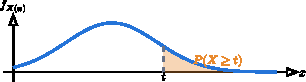
\includegraphics[keepaspectratio,alt={A density curve with the tail to the right of threshold t shaded as P(X \textgreater= t).}]{assets/fig-prob-04-lln-diagram-01.pdf}}
\caption{密度曲线在阈值 \(t\) 右侧的尾部概率}\label{fig-prob-04-lln-diagram-01}
\end{figure}

\end{qlremark}

\begin{proof}

我们考虑一个 indicator function \(\mathbf{1}_{\{{X \geq t}\}}\), 这也是 一个 non-negative random variable. 显然:

\[X \geq t \cdot \mathbf{1}_{\{{X \geq t}\}}\]

(在 \(X \geq t\) 的事件上等于, 其他事件上小于), 并且这个 indicator function 的 expectation 正是 \(X\) 大于 \(t\) 的概率 \({\mathbb{P}}(X \geq t)\).

因而 by linearity of expectation,

\[{\mathbb{E}}\lbrack X\rbrack \geq t{\mathbb{E}}\lbrack\mathbf{1}_{\{{X \geq t}\}}\rbrack = t{\mathbb{P}}(X \geq t)\]

其值为 1 当 \(X \geq t\) 时, 否则为 0. 对于任意的 \(t > 0\), 有

\end{proof}

% qlnotes: kind=corollary; id=cor-04-lln-chebyshevs-inequality; concepts=chebyshevs-inequality; aliases=Chebyshev’s inequality
\begin{corollary}{Chebyshev's inequality}\label{cor-04-lln-chebyshevs-inequality}

对于一个 random variable \(X\) 和任意的 \(t > 0\), 如果它的方差 \(\text{Var}(X)\) 是有限的, 那么 有

\[\left. {\mathbb{P}}( \middle| X - {\mathbb{E}}\lbrack X\rbrack \middle| \geq t) \leq \frac{\text{Var}(X)}{t^{2}} \right.\]

\end{corollary}

\begin{qlremark}{Remark}

Markov's ineq 是通过均值来 bound 非负随机变量 达到一定大小的概率 (在多少事件上是大于 \(t\) 的);

Chebyshev's ineq 则是通过方差来 bound 任意随机变量 偏离均值达到一定程度的概率 (在多少事件上是偏离均值超过 \(t\) 的).

\end{qlremark}

\begin{proof}

考虑 non-negative random variable \((X - {\mathbb{E}}\lbrack X\rbrack)^{2}\), 那么

\[\left. {\mathbb{P}}( \middle| X - {\mathbb{E}}\lbrack X\rbrack \middle| \geq t) = {\mathbb{P}}((X - {\mathbb{E}}\lbrack X\rbrack)^{2} \geq t^{2}) \leq \frac{{\mathbb{E}}\lbrack(X - {\mathbb{E}}\lbrack X\rbrack)^{2}\rbrack}{t^{2}} = \frac{\text{Var}(X)}{t^{2}} \right.\]

\end{proof}

\subsection{Cauchy-Schwarz and Jensen's ineq}\label{cauchy-schwarz-and-jensens-ineq}

% qlnotes: kind=theorem; id=thm-04-lln-cauchy-schwarz-inequality; concepts=cauchy-schwarz-inequality; aliases=Cauchy-Schwarz inequality
\begin{theorem}{Cauchy-Schwarz inequality}\label{thm-04-lln-cauchy-schwarz-inequality}

对于任意的 random variables \(X\) 和 \(Y\), 都有

\[\left. |{\mathbb{E}}\lbrack XY\rbrack \middle| \leq \sqrt{{\mathbb{E}}\lbrack X^{2}\rbrack \cdot {\mathbb{E}}\lbrack Y^{2}\rbrack} \right.\]

\end{theorem}

这是 prob space 作为一个 measure space, 其上的函数空间 \(L^{2}(\Omega,\mathcal{F},{\mathbb{P}})\) 作为一个 Hilbert space, 自然的 Cauchy-Schwarz inequality. 不赘述了.

% qlnotes: kind=theorem; id=thm-04-lln-jensens-inequality; concepts=jensens-inequality; aliases=Jensen’s inequality
\begin{theorem}{Jensen's inequality}\label{thm-04-lln-jensens-inequality}

对于一个 convex function \(\phi\) 和 任意的 random variable \(X\), 只要 \({\mathbb{E}}\lbrack X\rbrack\) 和 \({\mathbb{E}}\lbrack\phi(X)\rbrack\) 都是 well-defined 的 (即 finite), 都有

\[\phi({\mathbb{E}}\lbrack X\rbrack) \leq {\mathbb{E}}\lbrack\phi(X)\rbrack\]

\end{theorem}

\begin{proof}

Let \(x_{0} := {\mathbb{E}}\lbrack X\rbrack\).

Since \(\phi\) is convex, for any \(x\), there exists a supporting line to the graph of \(\phi\) at \(x\). 即 存在一个 \(m \in {\mathbb{R}}\) s.t. 对于任意的 \(y\), 都有

\[\varphi(x) \geq \varphi\left( x_{0} \right) + m\left( {x - x_{0}} \right)\]

因而 apply to \(X\), 我们 a.s. 有

\[\varphi(X) \geq \varphi({\mathbb{E}}\lbrack X\rbrack) + m(X - {\mathbb{E}}\lbrack X\rbrack)\]

因此 by linearity of expectation,

\[{\mathbb{E}}\lbrack\varphi(X)\rbrack \geq \varphi({\mathbb{E}}\lbrack X\rbrack) + m({\mathbb{E}}\lbrack X\rbrack - {\mathbb{E}}\lbrack X\rbrack) = \varphi({\mathbb{E}}\lbrack X\rbrack)\]

\end{proof}

\subsection{Fatou's Lemma, MCT and DCT}\label{fatous-lemma-mct-and-dct}

我们在 measure theory 中最熟悉的三个定理. 复习一下. 这里不 prove 了. proof 请左转 measure theory notes.

% qlnotes: kind=theorem; id=thm-04-lln-fatous-lemma; concepts=fatous-lemma; aliases=Fatou’s Lemma
\begin{theorem}{Fatou's Lemma}\label{thm-04-lln-fatous-lemma}

令 \(\left\{ X_{n} \right\}\) 是一列 non-negative random variables, 那么

\[{\mathbb{E}}\lbrack\operatorname{lim\, inf}\limits_{n\rightarrow\infty}X_{n}\rbrack \leq \operatorname{lim\, inf}\limits_{n\rightarrow\infty}{\mathbb{E}}\lbrack X_{n}\rbrack\]

\end{theorem}

\begin{qlremark}{Remark}

pointwise 下极限的积分, 得到的结果不会大于每个函数积分的下极限.

因为 pointwise 下极限即: 在每个 \(\omega\) 上, 整个序列中最终稳定的最低水平 , 这是最稳定的一层.

而逐个函数可能会有一些 spike, 使得它的 expectation 很大, 但是这个 spike 只出现有限次, 导致 pointwise limitinf 的函数没有受到它的影响; 但是, 不同的 spike 可能 finitely 出现在不同的位置上, 而这个出现的行为是无限的(比如 typewritter 函数), 使得每个函数的 expectation 都很大, 从而导致 expectation 的 limit 很大.

而 pointwise liminf 的 expectation 就是对每个点都取最终稳定的最低水平, 从而避免了这些 spikes 的影响.

\end{qlremark}

% qlnotes: kind=theorem; id=thm-04-lln-monotone-convergence-theorem-mct; concepts=monotone-convergence-theorem-mct; aliases=Monotone Convergence Theorem (MCT)
\begin{theorem}{Monotone Convergence Theorem (MCT)}\label{thm-04-lln-monotone-convergence-theorem-mct}

令 \(\left\{ X_{n} \right\}\) 是一列递增的 non-negative random variables (即 \(X_{n} \uparrow X\) a.s.), 那么 suppose \(X := \lim_{n\rightarrow\infty}X_{n}\) a.e. exists, 那么 a.s. 有

\[\lim\limits_{n\rightarrow\infty}{\mathbb{E}}\lbrack X_{n}\rbrack = {\mathbb{E}}\lbrack X\rbrack\]

\end{theorem}

\begin{qlremark}{Remark}

如果 \(X_{n}\) 是递减的, 那么 expectation 的 limit 就等于逐点 limit 的 expectation 了.

\end{qlremark}

% qlnotes: kind=theorem; id=thm-04-lln-dominated-convergence-theorem-dct; concepts=dominated-convergence-theorem-dct; aliases=Dominated Convergence Theorem (DCT)
\begin{theorem}{Dominated Convergence Theorem (DCT)}\label{thm-04-lln-dominated-convergence-theorem-dct}

令 \(\left\{ X_{n} \right\}\) 是一列 random variables, 并且存在一个 a.e. pointwise limit \(X\) (即 \(X_{n}\rightarrow X\) a.s.), 并且存在一个 integrable random variable \(Y\) 作为一个 bound: 使得 \(\left. |X_{n} \middle| \leq Y \right.\) a.s. 对所有的 \(n\) 成立,

那么

\[\lim\limits_{n\rightarrow\infty}{\mathbb{E}}\lbrack X_{n}\rbrack = {\mathbb{E}}\lbrack X\rbrack\]

\end{theorem}

\begin{qlremark}{Remark}

只要这个序列有一个 integrable 的 uniform bound (不要有很多 unbounded 的 spike 就行了), 那么 expectation 的 limit 就等于逐点 limit 的 expectation 了.

\end{qlremark}

\subsection{Tonneli and fubini}\label{tonneli-and-fubini}

% qlnotes: kind=theorem; id=thm-04-lln-tonnelis-theorem; concepts=tonnelis-theorem; aliases=Tonneli’s Theorem
\begin{theorem}{Tonneli's Theorem}\label{thm-04-lln-tonnelis-theorem}

对于一列 non-negative random variables \(\left\{ X_{n} \right\}\), 累加和积分(求期望)的顺序可以交换:

\[{\mathbb{E}}\left\lbrack {\sum\limits_{n = 1}^{+ \infty}X_{n}} \right\rbrack = \sum\limits_{n = 1}^{+ \infty}{\mathbb{E}}\left\lbrack X_{n} \right\rbrack\]

\end{theorem}

% qlnotes: kind=theorem; id=thm-04-lln-fubinis-theorem; concepts=fubinis-theorem; aliases=Fubini’s Theorem
\begin{theorem}{Fubini's Theorem}\label{thm-04-lln-fubinis-theorem}

对于一列任意的 random variables \(\left\{ X_{n} \right\}\), 只要其绝对值的 sum 的 expectation 是 finite 的 (或者绝对值的 expectation 的 sum 是 finite 的, by Tonneli 都是一样的), 那么就有 linearity of expectation 的推广:

\[{\mathbb{E}}\left\lbrack {\sum\limits_{n = 1}^{+ \infty}X_{n}} \right\rbrack = \sum\limits_{n = 1}^{+ \infty}{\mathbb{E}}\left\lbrack X_{n} \right\rbrack\]

\end{theorem}

\begin{qlremark}{Remark}

Fubini 和 Tonelli 即: 把 linearity of expectation 推广到 countable sum 的情况, 前提是 either 非负(因而无穷不用管) or 它们的 expectation 是一个绝对 收敛的 series 就行了.

\end{qlremark}

\section{Definition review: modes of convergence}\label{definition-review-modes-of-convergence}

这一个 section 也是一个 review. 讲讲 不同的 convergence mode 的定义, 以及它们之间的关系.

首先, 我们对 pointwise limit 和 uniform limit 的定义已经很熟悉了, 这里就不赘述了. (算了 uniform 还是提一嘴, 意思是我们需要 pointwise limit 的 收敛速度也是 uniform 的, 即对任意的 \(\epsilon > 0\), 都存在一个 \(N\) 使得对于所有的 \(n \geq N\) 和所有的 \(\omega\), 都有 \(\left. |X_{n}(\omega) - X(\omega) \middle| < \epsilon \right.\), 是一个严格强于 pointwise 的收敛方式. )

% qlnotes: kind=definition; id=def-04-lln-rv; concepts=rv; aliases=RV 序列的三种收敛方式
\begin{definition}{RV 序列的三种收敛方式}\label{def-04-lln-rv}

\begin{itemize}
\item
  \textbf{converge a.s. (almost surely)} 或称 converge with probability 1:

  \[{\mathbb{P}}\left( {\lim\limits_{n\rightarrow\infty}X_{n} = X} \right) = 1\]

  即:

  \[{\mathbb{P}}\left( \left\{ {\omega \in \Omega:\lim\limits_{n\rightarrow\infty}X_{n}(\omega) = X(\omega)} \right\} \right) = 1\]

  也就是说 \(X_{n}\) 的 a.e. pointwise limit 是 \(X\).
\item
  \textbf{converge in \(L^{p}\)}: 对于 \(L^{p}\)-integrable 的 random variables sequence \(X_{n}\) 和 \(X\), 我们称 \(X_{n}\overset{L^{p}}{\rightarrow}X\), 如果

  \[\lim\limits_{n\rightarrow\infty}{\mathbb{E}}\left\lbrack \left| {X_{n} - X} \right|^{p} \right\rbrack = 0\]

  即: 这个 seq of RVs 与这个 limit function 之间的 \(L^{p}\) distance 收敛到 0; 也就是它们的偏差 as a random variable, 其 \(p\)-th moment 收敛到 0.
\item
  \textbf{converge in probability}: 对于任意的 \(\epsilon > 0\), 如果

  \[\left. \lim\limits_{n\rightarrow\infty}{\mathbb{P}}( \middle| X_{n} - X \middle| > \epsilon) = 0 \right.\]

  即 \(X_{n}\) 与 \(X\) 之间的偏差超过 \(\epsilon\) 的概率收敛到 0.
\end{itemize}

\end{definition}

\section{Borel-Cantelli Lemma}\label{borel-cantelli-lemma}

\section{Laws of Large Numbers}\label{laws-of-large-numbers}

\subsection{weak and strong LLN}\label{weak-and-strong-lln}

下面是概率论中最重要的定律之一: 大数定律 (Laws of Large Numbers, LLN).

它证明的是一个十分符合直觉的结论: 一个 random variable 的 sample mean (即 \(n\) 个 i.i.d. 的 copy 的均值), 随着 sample 数量的增加, 会 converge to 它的 expectation.

就是说: 我们重复做一个相同的实验并 取结果的平均值, 当我们做的实验足够多时, 这个平均值就会非常接近于这个实验的 expectation, 也就是理论的均值.\\
例如最经典的例子就是抛硬币: 我们连续抛 \(n\) 次一个公平的硬币, 记录每次抛出正面 (记为 1) 或者反面 (记为 0), 然后计算这些结果的平均值, 随着 \(n\) 的增加, 这个平均值会趋近于 0.5, 等于 理论的 expectation (这是个 Bernouli random variable, expectation = \(p\)).\\
LLN 有两个阶段, weak LLN 和 strong LLN, weak LLN 证明的是这个 convergence 是 in probability 的, 而 strong LLN 证明的是这个 convergence 是 a.s. 的. 就是说 strong LLN 是严格强于 weak LLN 的.

% qlnotes: kind=theorem; id=thm-04-lln-weak-law-of-large-numbers; concepts=weak-law-of-large-numbers; aliases=weak Law of Large Numbers
\begin{theorem}{weak Law of Large Numbers}\label{thm-04-lln-weak-law-of-large-numbers}

对于一列 i.i.d. 的 random variables \(\left\{ X_{i} \right\}\), 只要这个 random variable 的 expectation 是 finite 的 \({\mathbb{E}}\lbrack X_{1}^{2}\rbrack < \infty\), 那么就有:

\[\frac{X_{1} + X_{2} + \cdots + X_{n}}{n}\overset{p}{\rightarrow}{\mathbb{E}}\lbrack X_{1}\rbrack\quad\text{as}\ n\rightarrow\infty\]

\end{theorem}

\begin{proof}

简写 \(\mu := {\mathbb{E}}\lbrack X_{1}\rbrack\), \(S_{n} := \frac{X_{1} + X_{2} + \cdots + X_{n}}{n}\) for each \(n\).

Let \(\varepsilon > 0\). It suffices to show: \(\left. {\mathbb{P}}( \middle| S_{n} - \mu \middle| > \varepsilon)\rightarrow 0 \right.\) as \(n\rightarrow\infty\). By Chebyshev's inequality, we have

\[\begin{matrix}
{{\mathbb{P}}\left( {\left| {S_{n}/n - \mu} \right| > \varepsilon} \right)} & {\leq \frac{\text{Var}(S_{n}/n)}{\varepsilon^{2}}} \\
 & {= \frac{1}{n^{2}\varepsilon^{2}}\left( \sum\limits_{n = 1}^{n}{\mathbb{E}}\lbrack \middle| \ X_{i} - \mu\  \middle| {}_{2}\rbrack + 2\sum\limits_{1 \leq i < j \leq n}{\mathbb{E}}\lbrack(X_{i} - \mu)(X_{j} - \mu)\rbrack \right)}
\end{matrix}\]

notice: 由于每个 \(X_{i}\) 都是 i.i.d. 的, independence \(\Longrightarrow\) uncorrelatedness \(\Longrightarrow\text{Cov}(X,Y) = {\mathbb{E}}\lbrack XY\rbrack - {\mathbb{E}}\lbrack X\rbrack{\mathbb{E}}\lbrack Y\rbrack = 0\), 因而 \({\mathbb{E}}\lbrack(X_{i} - \mu)(X_{j} - \mu)\rbrack = {\mathbb{E}}\lbrack(X_{i} - \mu)\rbrack{\mathbb{E}}\lbrack(X_{j} - \mu)\rbrack = 0 \cdot 0 = 0\) for each \(i \neq j\).

因而

\[\left. {\mathbb{P}}\left( {\left| {S_{n}/n - \mu} \right| > \varepsilon} \right) = \frac{1}{\varepsilon^{2}n^{2}}\sum\limits_{n = 1}^{n}{\mathbb{E}}\lbrack \middle| X_{i} - \mu \middle| {}_{2}\rbrack = \frac{1}{\varepsilon^{2}n} \cdot n\ \text{Var}(X_{1})\overset{n\rightarrow\infty}{\rightarrow}0 \right.\]

\end{proof}

% qlnotes: kind=theorem; id=thm-04-lln-strong-law-of-large-numbers; concepts=strong-law-of-large-numbers; aliases=strong Law of Large Numbers
\begin{theorem}{strong Law of Large Numbers}\label{thm-04-lln-strong-law-of-large-numbers}

在 weak LLN\hyperref[thm-04-lln-weak-law-of-large-numbers]{Theorem~\ref*{thm-04-lln-weak-law-of-large-numbers}} 的相同条件 (其实可以更弱, 让 \(E\lbrack X_{1}\rbrack < \infty\) 即可) 下, 我们其实可以得到一个更强的结论:

\[\frac{X_{1} + \ldots + X_{n}}{n}\overset{\text{a.s.}}{\rightarrow}{\mathbb{E}}\left\lbrack X_{1} \right\rbrack,\quad\text{as}\ n\rightarrow\infty\]

\end{theorem}

\begin{proof}

For simplicity, 我们不证明更弱的条件 (\(E\lbrack X_{1}\rbrack < \infty\)) 下的 strong LLN 了. 只沿用相同的条件.

简写 \(\mu := {\mathbb{E}}\lbrack X_{1}\rbrack\), \(\sigma^{2} := \text{Var}(X_{1})\), \(S_{n} := \frac{X_{1} + X_{2} + \cdots + X_{n}}{n}\) for each \(n\), 以及

\[Y_{n} := \frac{S_{n}}{n} - \mu\]

我们将要证明: \(Y_{n}\overset{a.s.}{\rightarrow}0\).

首先, 在 weak LLN 的 proof 中, 我们已经证明了:

\[{\mathbb{E}}(Y_{n}) = 0,\quad{\mathbb{E}}\lbrack Y_{n}^{2}\rbrack = \frac{\sigma^{2}}{n}\]

我们发现: 当我们只采样 \(n^{2}\) indexed 的时候, 它们的 expectation 的 sum 是 finite 的, by p-test (因为 \(\sum_{n = 1}^{\infty}\frac{1}{n^{p}}\) 收敛当且仅当 \(p > 1\)), 即:

\[{\mathbb{E}}\left\lbrack {\sum\limits_{n = 1}^{+ \infty}Y_{n^{2}}^{2}} \right\rbrack = \sum\limits_{n = 1}^{+ \infty}{\mathbb{E}}\left\lbrack Y_{n^{2}}^{2} \right\rbrack = \sum\limits_{n = 1}^{+ \infty}\frac{\sigma^{2}}{n^{2}} < \infty\]

先考虑所有 \(Y_{n}\) 都非负的 case. 我们知道: expectation of 一个 non-negative random variable 是 finite 的, 就 imply 它是 a.e. finite 的. 因而

\[\sum\limits_{n = 1}^{+ \infty}Y_{n^{2}}^{2} < \infty\quad\text{a.s.}\]

因而

\[\lim\limits_{n\rightarrow\infty}Y_{n^{2}} = 0\quad\text{a.s.}\]

意味把在 \(1,4,9,16...\) 这些 index 的 \(Y_{i}\) 求 average, 确实收敛到了 \(\mu\).

而我们可以通过 squeeze theorem 得到 general case: 对于任意正整数 \(k\), 总能找到一对平方数把它夹在中间. 比如令 \(n^{2} < k < (n + 1)^{2}\).

我们发现:

\[\frac{S_{n^{2}}}{(n + 1)^{2}} \leq \frac{S_{k}}{k} \leq \frac{S_{(n + 1)^{2}}}{n^{2}}\]

notice: \(\frac{S_{n^{2}}}{(n + 1)^{2}} = \frac{S_{n^{2}}}{n^{2}} \cdot \frac{n^{2}}{(n + 1)^{2}}\), 前向 converge to \(\mu\), 后向 converge to 1, 因而 \(\frac{S_{n^{2}}}{(n + 1)^{2}}\rightarrow\mu\), 后面那个也同理. 因而夹逼得到 \(S_{k}/k\rightarrow\mu\). 从而得证.

General case:

\[X_{n} = \max\left\{ {X_{n},0} \right\} - \max\left\{ {- X_{n},0} \right\} = :X_{n}^{+} - X_{n}^{-}\]

因而

\[\frac{X_{1} + \ldots + X_{n}}{n} = \frac{X_{1}^{+} + \ldots + X_{n}^{+}}{n} - \frac{X_{1}^{-} + \ldots + X_{n}^{-}}{n}\overset{\text{a.s.}}{\rightarrow}{\mathbb{E}}\left\lbrack X_{1}^{+} \right\rbrack - {\mathbb{E}}\left\lbrack X_{1}^{-} \right\rbrack = {\mathbb{E}}\left\lbrack X_{1} \right\rbrack\]

得证.

\end{proof}

\begin{qlremark}{Remark}

我们要求 \(\left. {\mathbb{E}}\lbrack \middle| X_{1} \middle| \rbrack \right.\) 是 finite 的, 或者 \(\left. {\mathbb{E}}\lbrack \middle| X_{1} \middle| {}_{2}\rbrack \right.\) 是 finite 的, 并不是一个硬性的条件, 只是结果确实 converge to \({\mathbb{E}}\lbrack X_{1}\rbrack\) 这个 finite value 的条件.

实际上在 \({\mathbb{E}}\lbrack X_{1}\rbrack\) infinite (等于 \(\infty\) 或者 \(- \infty\)) 时, 我们会得到这个 average 发散, 因而也是 和 \({\mathbb{E}}\lbrack X_{1}\rbrack\) 一样, 只不过不是 converge 而是 diverge.

此处不证明了.

\end{qlremark}

\subsection{application: Monte Carlo methods}\label{application-monte-carlo-methods}

任何利用 LLN 来近似计算 一个 quantity 的方法, 都可以称之为 Monte Carlo 方法.

它的核心思想是:

\begin{itemize}
\item
  选择一个随机变量, 其 expectation 等于我们要计算的 quantity.
\item
  大量重复采样这个随机变量, 并计算样本的平均值
\item
  根据大数定律, 这个平均值近似于我们要计算的 quantity.
\item
  我们可以用 Chebyshev's inequality 来给出这个近似的误差 bound.
\end{itemize}

% qlnotes: kind=example; id=ex-04-lln-pi; concepts=-pi; aliases=估算 \pi
\begin{example}[估算 pi]\label{ex-04-lln-pi}

我们令 \(X,Y \sim U(\lbrack - 1,1\rbrack)\)

那么

\[{\mathbb{E}}\left\lbrack {\mathbf{1}_{C}(X,Y)} \right\rbrack = \int_{- 1}^{1}\int_{- 1}^{1}\mathbf{1}_{C}(x,y)f_{X,Y}(x,y)dxdy = \frac{1}{4}\int_{- 1}^{1}\int_{- 1}^{1}\mathbf{1}_{C}(x,y)dxdy = \frac{\pi}{4}\]

注意我们每次随机采样 \(X,Y\) 的时候, 都是在 \(\lbrack - 1,1\rbrack \times \lbrack - 1,1\rbrack\) 这个正方形里随机选一个点, 即创建了一个 random variable \((X_{i},Y_{i})\) 并进行观测.

根据 LLN, 不论单次的采样结果如何, 我们都可以得到

\[\lim\limits_{n\rightarrow\infty}\frac{\mathbf{1}_{C}\left( {X_{1},Y_{1}} \right) + \ldots + \mathbf{1}_{C}\left( {X_{n},Y_{n}} \right)}{n} = \frac{\pi}{4},\quad\text{a.s.}\]

我们还可以用 Chebyshev's inequality 来给出这个近似的误差 bound:

\[{\mathbb{P}}\left( {\left| {4S_{n}/n - \pi} \right| > \varepsilon} \right) \leq \frac{\text{Var}\ \left( {4S_{n}/n} \right)}{\varepsilon^{2}} = \frac{4^{2}}{n^{2}\varepsilon^{2}}\ \text{Var}\ \left( {\sum\limits_{i = 1}^{n}\mathbf{1}_{C}\left( {X_{i},Y_{i}} \right)} \right) = \frac{16}{n\varepsilon^{2}}\ \text{Var}\ \left( {\mathbf{1}_{C}\left( {X_{1},Y_{1}} \right)} \right) \approx \frac{1}{n\varepsilon^{2}}\]

因而当 \(n\) 足够大时, 几乎一定可以得到目标值.

\begin{verbatim}
import random
def estimate_pi(n):
    S_n = 0 # This step 1
    for _ in range(n):
        # Here is step 2 (and 3)
        X = random.uniform(-1, 1)
        Y = random.uniform(-1, 1)
        # Check if the point is inside the unit circle
        if X**2 + Y**2 <= 1:
            S_n += 1
    pi_estimate = 4 * S_n / n
    return pi_estimate
# Example usage
n = 1000000
pi_approx = estimate_pi(n)
print(pi_approx)
\end{verbatim}

\end{example}

\subsection{application: Bernstein Polynomials}\label{application-bernstein-polynomials}

\subsection{application: Hypothesis testing}\label{application-hypothesis-testing}

\chapter{Central Limit Theorem}\label{central-limit-theorem}

\section{convergence in distribution}\label{convergence-in-distribution}

% qlnotes: kind=definition; id=def-05-clt-convergence-in-distribution; concepts=convergence-in-distribution; aliases=convergence in distribution
\begin{definition}{convergence in distribution}\label{def-05-clt-convergence-in-distribution}

我们称一个 seq of random variables \(\left\{ X_{n} \right\}\) converge in distribution to a random variable \(X\), 写作 \(X_{n}\overset{d}{\rightarrow}X\), 如果 \(X\) 的 分布函数 \(F_{X}\) 下所有 右连续的 \(x\) (即 \(F_{X}(x) = F_{X}(x - )\) ), 都有

\[\lim\limits_{n\rightarrow\infty}F_{X_{n}}(x) = F_{X}(x)\]

\end{definition}

\begin{qlremark}{Remark}

Convergence in distribution 的意思就是: 随着 \(n\) 越来越大, \(X_{n}\) 的分布是否越来越接近 \(X\) 的分布. 这是一个非常弱的收敛概念, 因为它甚至\textbf{不要求 \(X_{n}\) 和 \(X\) 在同一个概率空间上定义,} 也不要求 \(X_{n}\) 和 \(X\) 之间有任何关系. 只需要 分布函数收敛即可.

并且 notice: 并不要求对所有点 \(x\) 都有 \(F_{X_{n}}(x)\rightarrow F_{X}(x)\), 而是只要求对 \(X\) 的分布函数 \(F_{X}\) 下所有右连续的点 \(x\). 这是因为如果不加这个限制, 很多直观上应该收敛的情况在数学上就会失败.

比如: 令\(X_{n} = 1/n\), 一个 constant random variable, 那么 \(X_{n}\) 的分布函数 \(F_{X_{n}}\) 是一个 step function. 但是在 \(x = 0\) 处, \(F_{X_{n}}(0) = 0\) for all \(n\), 因而 \(\lim_{n\rightarrow\infty}F_{X_{n}}(0) = 0\).

而 \(F_{X}(0) = 1\).

所以对于这种跳跃不连续点, 如果不跳过, 那么就会得出 \(X_{n}\) 不收敛于 \(X\) 的错误结论. 但是我们知道, 分布函数作为一个单调递增的函数, 是 a.e. continuous 的, 因而这些点是可以忽略掉的.

\end{qlremark}

\section{Characterization of a distribution}\label{characterization-of-a-distribution}

\subsection{moment generating function}\label{moment-generating-function}

% qlnotes: kind=definition; id=def-05-clt-moment-generating-function; concepts=moment-generating-function; aliases=moment generating function
\begin{definition}{moment generating function}\label{def-05-clt-moment-generating-function}

对于一个随机变量 \(X\), 其 moment generating function (MGF) 定义为

\[M_{X}(t) = {\mathbb{E}}\lbrack e^{tX}\rbrack,\quad t \in {\mathbb{R}}\]

\end{definition}

\begin{qlremark}{Remark}

为什么这个东西叫做 moment generating function 呢? 因为如果 \(M_{X}(t)\) 在 \(t = 0\) 的某个 neighborhood 内存在, 那么我们可以通过对 \(M_{X}(t)\) 求导来得到 \(X\) 的各阶矩:

\end{qlremark}

% qlnotes: kind=proposition; id=prop-05-clt-proposition-001; concepts=proposition-001
\begin{proposition}\label{prop-05-clt-proposition-001}

如果 \(M_{X}(t)\) 在 \(t = 0\) 的某个 neighborhood 内存在, 则 \(X\) 的 \(n\) 阶矩可以表示为

\[{\mathbb{E}}\lbrack X^{n}\rbrack = M_{X}^{(n)}(0)\]

其中 \(M_{X}^{(n)}(0)\) 表示 \(M_{X}(t)\) 在 \(t = 0\) 处的 \(n\) 阶导数.

\end{proposition}

\subsection{characteristic function}\label{characteristic-function}

\section{Central Limit Theorem}\label{central-limit-theorem-1}

% qlnotes: kind=theorem; id=thm-05-clt-lindeberg-levy-central-limit-theorem; concepts=lindeberg-levy-central-limit-theorem; aliases=Lindeberg-Levy Central Limit Theorem
\begin{theorem}{Lindeberg-Levy Central Limit Theorem}\label{thm-05-clt-lindeberg-levy-central-limit-theorem}

对于任意一个 seq of i.i.d. random variables \(\left\{ X_{i} \right\}\) with mean \(\mu\) and variance \(\sigma^{2} < \infty\), set \(S_{n} = X_{1} + X_{2} + \cdots + X_{n}\) for each \(n\).

我们有:

\[\frac{S_{n} - n\mu}{\sqrt{n\sigma^{2}}}\overset{d}{\rightarrow}N(0,1)\]

\end{theorem}

\begin{qlremark}{Remark}

LLN 告诉我们, 当 \(n\) 越来越大时, \(S_{n}/n\) 越来越接近 \(\mu\). 每个 \(X_{i}\) 随机取样, 不论结果如何, 其平均值大概率都是 \(\mu\).\\
CLT 则是进一步告诉我们这个接近的过程是如何发生的: 随着 \(n\) 越来越大, \(S_{n}\) 的分布会越来越接近一个正态分布, 且波动的幅度(标准差)数量级为 \(\sqrt{n}\). \textbf{因而平均值 \(S_{n}/n\) 的分布会越来越接近一个均值为 \(\mu\), 标准差为 \(\sigma/\sqrt{n}\) 的正态分布}

\[\frac{S_{n}}{n} = \mu + \frac{\sigma}{\sqrt{n}}Z,\quad Z \sim N(0,1)\]

\textbf{随着\(n\) 越来越大, 这个标准差会越来越小, 因而 其极限坍缩为一个 constant \(\mu\).}\\

\end{qlremark}

\begin{qlremark}{Remark}

CLT 的一个主要的应用价值, 就是可以用来估计 由多个 i.i.d. 随机因素共同作用的现象的分布.

统计学中常用于对 confidence interval 的估计, 以及 hypothesis testing, 通过计算如 \({\mathbb{P}}\left( {\frac{S_{n} - n\mu}{\sqrt{n\sigma^{2}}} \in A} \right)\) 这种形式的概率来进行推断.\\

\end{qlremark}

在进行证明前, 我们先看一些 applications of CLT. 可能会帮助我们更好地理解 CLT 的意义.

\subsection{applications of CLT}\label{applications-of-clt}

% qlnotes: kind=example; id=ex-05-clt-coin-fair; concepts=-coin-fair; aliases=(判断 coin 是否 fair)
\begin{example}[(判断 coin 是否 fair)]\label{ex-05-clt-coin-fair}

我们有两个 coins, 想要判断它们是否是 fair coin. 我们可以 toss 这个 coin \(n\) 次, 记录下每次 toss 的结果, 记为 \(X_{1},X_{2},\cdots,X_{n}\), 其中 \(X_{i} = 1\) if the \(i\)-th toss is heads.

现在: 观测到第一个 coin 100 次 toss 中有 38 次是 heads, 第二个 coin 100 次 toss 中有 43 次是 heads.

\begin{qlsolution}{Solution}

假设这两个 coins 是 fair coin. 那么 \(X_{i}\) 是 i.i.d. Bernoulli random variables with parameter \(p = 0.5\), 因而 \(\mu = p = \frac{1}{2}\), \(\sigma^{2} = p(1 - p) = \frac{1}{4}\). 从而根据 CLT,

\[{\mathbb{P}}(S_{100} < 38) = {\mathbb{P}}\left( {\frac{S_{100} - 100 \cdot \frac{1}{2}}{\sqrt{100 \cdot \frac{1}{4}}} < \frac{38 - 100 \cdot \frac{1}{2}}{\sqrt{100 \cdot \frac{1}{4}}}} \right) \approx {\mathbb{P}}\left( {Z < \frac{38 - 50}{5}} \right) \approx {\mathbb{P}}(Z < - 2.4) \approx 0.0082 < 0.01\]

因而这个第一个 coin 很可能不是 fair coin. 同样的方法计算出 \({\mathbb{P}}\left( {S_{100} \leq 43} \right) \approx 0.0887\), 因而第二个 coin 虽然也可疑不是 fair coin, 但是不如第一个 coin 可疑. 如果以 0.05 作为显著性水平, 那么我们可以拒绝第一个 coin 是 fair coin 的假设.\\

\end{qlsolution}

\end{example}

% qlnotes: kind=example; id=ex-05-clt; aliases=(样本量需求的计算)
\begin{example}[(样本量需求的计算)]\label{ex-05-clt}

工厂生产了一批电线, 我们想知道它们的平均断裂强度 \(\mu\) 是多少. 遂抽取 \(n\) 根电线进行测量, 得到 \(X_{1},...,X_{n}\), 然后计算它们的样本平均值 \({\bar{X}}_{n}\) 来估计 \(\mu\).

已知量: 强度的方差 \(\sigma^{2} = 1/10\).; 我们想估计的是 \(\mu\) 的值. 并且我们希望我们的估计是准的, in the sense that: 误差 \(|{\bar{X}}_{n} - \mu|\) 不超过 0.01 的概率至少为 0.95.

\begin{qlsolution}{Solution}

我们要达到: \(\left. {\mathbb{P}}( \middle| {\bar{X}}_{n} - \mu \middle| \leq 1/100) \right.\).

我们要把它转成标准的 normal distribution 的形式, 即 \(Z = \frac{S_{n} - n\mu}{\sqrt{n\sigma^{2}}}\) 的形式.

于是我们把 \({\bar{X}}_{n} - \mu\) 写为 \(\frac{S_{n}}{n} - \mu\), 然后两边同时乘 \(\frac{\sqrt{n}}{\sigma}\). 右边的常数项也做相同的变换: \(\frac{1/100}{\sigma/\sqrt{n}} = \frac{\sqrt{n}}{100\sigma}\).

于是原式变为:

\[\left. {\mathbb{P}}( \middle| Z \middle| \leq \frac{\sqrt{n}}{100\sigma}) \approx 0.95 \right.\]

对于正态分布我们知道

\[\left. {\mathbb{P}}( \middle| Z \middle| \leq x) = 2\Phi(x) - 1 \right.\]

于是想要:

\[2\Phi\left( \frac{\sqrt{n}}{100\sigma} \right) - 1 \geq 0.95\Longrightarrow\Phi\left( \frac{\sqrt{n}}{100\sigma} \right) \geq 0.975\]

通过查表我们知道当 \(\Phi(z) = 0.975\) 时, \(z \approx 1.96\). 因此要求 \(\frac{\sqrt{n}}{100\sigma} \geq 1.96\), 解得至少需要 \(n \geq (61.98)^{2} \approx 384.16\), floor 一下得到 \(n \geq 385\).

\end{qlsolution}

\begin{qlremark}{Remark}

这里的应用正是我们开头说的: LLN 告诉我们, 当 \(n\) 越来越大时, \(S_{n}/n\) 越来越接近 \(\mu\). 每个 \(X_{i}\) 随机取样, 不论结果如何, 其平均值大概率都是 \(\mu\); 而 CLT 则是进一步告诉我们这个接近的过程是如何发生的:

\[\frac{S_{n}}{n} = \mu + \frac{\sigma}{\sqrt{n}}Z,\quad Z \sim N(0,1)\]

随着\(n\) 越来越大, 这个标准差会越来越小, 因而 其极限坍缩为一个 constant \(\mu\). \textbf{因而, 我们可以通过 CLT 来得到: 我们 要用样本均值来估计分布的真实均值的话, 在一定的置信水平下, 需要多少样本量 \(n\) 才能保证我们的估计是准的.}

\end{qlremark}

\end{example}

\subsection{Berry-Esseen Theorem: CLT 的收敛速度}\label{berry-esseen-theorem-clt-ux7684ux6536ux655bux901fux5ea6}

之前的例子中, 我们都 使用了 \(\approx\) 表示: 我们直接把此时的分布近似当作了一个 normal distribution, 来计算一些概率.

但是: 这两个分布的近似行为的本身有多么精准?

下面有一个 theorem 刻画了这件事.

% qlnotes: kind=theorem; id=thm-05-clt-berry-esseen-theorem; concepts=berry-esseen-theorem; aliases=Berry-Esseen Theorem
\begin{theorem}{Berry-Esseen Theorem}\label{thm-05-clt-berry-esseen-theorem}

给定一个 seq of i.i.d. random variables \(\left\{ X_{i} \right\}\) with mean \(\mu\) and variance \(\sigma^{2} < \infty\), 以及 \(\left. {\mathbb{E}}\lbrack \middle| X_{i} - \mu \middle| {}_{3}\rbrack = \rho < \infty \right.\), set \(S_{n} = X_{1} + X_{2} + \cdots + X_{n}\), 我们有: 对于任意 \(x \in {\mathbb{R}}\),

\[\left| {{\mathbb{P}}\left( {\frac{S_{n} - n\mu}{\sqrt{n\sigma^{2}}} \leq x} \right) - \Phi(x)} \right| \leq \frac{3\rho}{\sigma^{2}\sqrt{n}}\]

\end{theorem}

\begin{qlremark}{Remark}

给定一个 number of samples \(n\), 我们可以给出此时的 真实概率与正态近似值之间的差值的 一个 upper bound.\\
并且, 这个 bound 不是概率意义上的 bound, 而\textbf{是一个 deterministic bound, 没有任何的随机性}; 并且是 \textbf{uniform across all \(x\) 的 bound.}\\
这是因为这里本身就是两个概率的值之间的差, 而不是样本之间的差. 因而其实这是一个非常强大的 结论, 表面\textbf{我们用正态分布近似估计出的概率 和真实的概率之间的差值是 determinstically controllable 意义上非常小的.}\\
我们马上可以想到: 对于 控制样本数量来达到某个置信水平的问题, 这是一个非常有用的工具, 因为它告诉我们, 当 \(n\) 足够大时, 我们用正态分布近似估计出的概率和真实的概率之间的 差值是非常小并且可以控制的.\\
并且, 这个控制应该是比较精准的. 因为相比其他的控制方法: \textbf{Chebyshev 只需要 first, second order moments 的信息; Hoeffding 只需要有界性的假设, 甚至不需要知道 分布的任何 moment 信息; 而 Berry-Esseen 需要 third order moment 的信息, 因此它应该能够给一个更精准的控制.}

\end{qlremark}

\begin{proof}

//TODO:

\end{proof}

% qlnotes: kind=example; id=ex-05-clt-example-003; concepts=example-003
\begin{example}\label{ex-05-clt-example-003}

一个工厂生产电子元件, 每个原件有概率是有缺陷的.

令

\[X_{i} = \left\{ \begin{matrix}
{1,} & {\text{if the}\ i\ \text{th tested component is defective},} \\
{0,} & {\text{otherwise}\ .}
\end{matrix} \right.\]

并假设 i.i.d. with parameter

\[{\mathbb{P}}(X_{i} = 1) = p\]

其中 \(p\) 是一个未知的参数.

工厂方面表示这个 process 是 under control 的, 并给出了假设: \(H_{0}:p \leq 0.02\).

为了验证这个假设, 一个 quality control manager 需要从生产线上需要随机 \(n\) 个元件进行测试, 并估计出 \(p\) 的值 by 样本均值:

\[{\widehat{p}}_{n} := \frac{1}{n}\sum\limits_{i = 1}^{n}X_{i}\]

我们希望这个估计的误差最多为 0.005, 并且这个误差的置信度至少为 0.99, 即我们希望:

\[{\mathbb{P}}\left( {\left| {{\widehat{p}}_{n} - p} \right| > 0.005} \right) \leq 0.01\]

那么我们至少需要多少样本量 \(n\) 来达到这个要求呢?

\end{example}

\begin{qlsolution}{Solution}

首先计算样本均值 \({\widehat{p}}_{n}\) 的 mean 和 variance:

\[{\mathbb{E}}\left\lbrack {\widehat{p}}_{n} \right\rbrack = p,\quad\text{Var}\ \left( {\widehat{p}}_{n} \right) = \frac{1}{n^{2}}\sum\limits_{i = 1}^{n}\text{Var}\ \left( X_{i} \right) = \frac{p(1 - p)}{n}\]

此时我们有三个办法:

\begin{itemize}
\item
  办法1: \textbf{Chebyshev's inequality}.

  \[{\mathbb{P}}\left( {\left| {{\widehat{p}}_{n} - p} \right| \geq \varepsilon} \right) \leq \frac{\text{Var}\ \left( {\widehat{p}}_{n} \right)}{\varepsilon^{2}} = \frac{p(1 - p)}{n\varepsilon^{2}}\]

  由于 \(p(1 - p) \leq 1/4\) for any \(p \in \lbrack 0,1\rbrack\), 式子可以进一步控制为

  \[{\mathbb{P}}\left( {\left| {{\widehat{p}}_{n} - p} \right| \geq \varepsilon} \right) \leq \frac{1}{4n\varepsilon^{2}}\]

  我们希望此概率不超过 0.01, 并且~\(\varepsilon = 0.005\), 那么进一步得到需要

  \[\frac{1}{4n(0.005)^{2}} \leq 0.01\]

  解得至少需要 \(n \geq 1000000\).
\item
  办法2: \textbf{Hoeffding's inequality}.\\
  由于 \(0 \leq X_{i} \leq 1\), 我们可以直接使用 Hoeffding's inequality 来控制:

  \[{\mathbb{P}}\left( {\left| {{\widehat{p}}_{n} - p} \right| \geq \varepsilon} \right) \leq 2e^{- 2n\varepsilon^{2}}\]

  我们 require 了 \(2e^{- 2n(0.005)^{2}} \leq 0.01\), 因而可以解得

  \[n \geq \frac{|\ln(0.005)|}{2(0.005)^{2}} \approx 106,000\]
\item
  办法3: \textbf{Berry-Esseen Theorem}.\\
  首先我们假设报告的 \(p\) 的值 0.02 是正确的, 从而可以计算出:

  \[{\mathbb{E}}\left\lbrack X_{1} \right\rbrack = p,\quad\sigma^{2} := \text{Var}\ \left( X_{1} \right) = p(1 - p) = 0.0196,\quad\sigma = 0.14\]

  并且, 由于 \(\left| {X_{1} - p} \right| \leq 1\), 我们知道偏度 \(\rho := {\mathbb{E}}\left\lbrack \left| {X_{1} - p} \right|^{3} \right\rbrack < \infty\).

  因而可以应用 Berry-Esseen Theorem. 我们希望:

  \[{\mathbb{P}}\left( {\left| {{\widehat{p}}_{n} - p} \right| \leq \varepsilon} \right) = {\mathbb{P}}\left( {\left| {S_{n} - np} \right| \leq n\varepsilon} \right) \geq 0.99,\quad\varepsilon = 0.005\]

  等价于

  \[{\mathbb{P}}\left( {\left| \frac{S_{n} - np}{\sigma\sqrt{n}} \right| \leq \frac{\varepsilon\sqrt{n}}{\sigma}} \right) \geq 0.99\]

  Berry-Esseen Theorem 可以得到: 对于任意的 \(x > 0\), 有

  \[{\mathbb{P}}\left( {\left| \frac{S_{n} - np}{\sigma\sqrt{n}} \right| \leq x} \right) \geq 2\Phi(x) - 1 - \frac{6\rho}{\sigma^{2}\sqrt{n}}\]

  因而我们需要选择 \(n\) s.t.

  \[2\Phi\left( \frac{\varepsilon\sqrt{n}}{\sigma} \right) - 1 - \frac{6\rho}{\sigma^{2}\sqrt{n}} \geq 0.99\]

  忽略掉 \(\frac{6\rho}{\sigma^{2}\sqrt{n}}\) 这个很小的项 (计算可以再精细地选择 \(n\)), 我们也可以得到:

  \[\frac{\varepsilon\sqrt{n}}{\sigma} \geq z_{0.995} \approx 2.576\]

  因而至少需要 \(n \geq 5200\).
\end{itemize}

我们可以看到

\begin{itemize}
\item
  通过 Chebyshev's inequality 来控制, 我们需要的样本量是 100 万级别的;
\item
  通过 Hoeffding's inequality 来控制, 我们需要的样本量是 10 万级别的;
\item
  通过 Berry-Esseen Theorem 来控制, 我们需要的样本量是 5000 级别的, 显然更为高效.
\end{itemize}

不过, 这个结果是基于我们假设 \(p = 0.02\) 的前提下得到的. Chebyshev 的逻辑 (保守估计): 我不相信厂家的任何话, 我要建立一个无论真实 \(p\) 是多少都绝对成立的置信区间. 所以我必须用最差的情况 \(p = 0.5\) 来算 \(n\). CLT/Berry-Esseen 的逻辑 (假设检验): 厂家宣称 \(p \leq 0.02\). 在统计学中, 我们通常先假设这个宣称是正确的 (即 \(H_{0}\) 假设). 如果我们用在这个假设下得出的需要的样本量 \(n = 5200\) 去测, 发现结果远超 \(0.02\), 那我们就直接推翻厂家的说法.

\end{qlsolution}

\subsection{proof of CLT}\label{proof-of-clt}

\printbibliography
\end{document}
